\documentclass[letterpaper,12pt]{book}

%%%%%%%%%%%%%%%%%%%%%%%%%%%%%% LyX specific LaTeX commands.
%\newcommand{\noun}[1]{\textsc{#1}}
%\providecommand{\tabularnewline}{\\}

\usepackage{mystyle}

\begin{document}
\begin{titlepage} %portada
  \thispagestyle{empty} %borrar el formato de pagina linda
  \begin{flushleft} %alinear a la izq
    %\begin{center}
    
\includegraphics[scale=0.35]{PTI.jpg}
    %\end{center}
  \end{flushleft}
  \vfill
  \vspace{2cm} %espacio vertical , en realidad es un enter de 2 cm
  \begin{center} %centrar
    {
      %    \begin{figure}[H]
      %      \centering
      %      \includegraphics[width=0.4\textwidth]{.png}
      %      \label{fig:Phyrex}
      %    \end{figure}
      \Huge Tutorial Diario\\
      %      \begin{figure}[H]
      %        \centering
      %        
\includegraphics[width=0.2\textwidth]{PTI.jpg}
      %        \label{fig:umce}
      %      \end{figure}
      %      \normalsize \today
    }
  \end{center}

  \vspace{5cm}

  \begin{figure}[H]
    \centering
    \begin{subfigure}[b]{0.2\textwidth}
      \centering
      
\includegraphics[width=\textwidth]{PaisDigital.jpg}
      \label{fig:Viper}
    \end{subfigure}
    ~
%    ~
%    \begin{subfigure}[b]{0.4\textwidth}
%      \centering
%      
\includegraphics[width=\textwidth]{Samsung.png}
%      \label{fig:Phyrex}
%    \end{subfigure}
    \begin{subfigure}[b]{0.23\textwidth}
      \centering
      
\includegraphics[width=\textwidth]{SamsungTechInstitute.jpg}
      \label{fig:Viper}
    \end{subfigure}
    ~\\
    \begin{subfigure}[b]{0.4\textwidth}
      \centering
      
\includegraphics[width=\textwidth]{InriaChile.png}
      \label{fig:Phyrex}
    \end{subfigure}
  \end{figure}

  \vfill
%  \begin{table}[H]
%    \centering
%    \begin{tabular}{rl}
%      Alumnos: & Karina Piumarta Echeverría\\
%      & Nicolás Manzano Reyes\\
%      &\\
%      Profesor Guía: &Ivan Correa Sierra \\
%    \end{tabular}
%  \end{table}
\end{titlepage}

\pagenumbering{Roman} %numero de paginas de indices en numeros romanos
\tableofcontents %indice de capitulos, secciones y subsecciones
\listoffigures   %indice de imagenes
\cleardoublepage
\listoftables    %indice de tablas
\cleardoublepage

\pagenumbering{arabic} %numeracion en numeros arabicos
\setcounter{page}{1} %empezar enumerando la pagina 1
\chapter*{Introducción}
Hola! Bienvenido a tu primer día en el taller de programación Programa
Tus Ideas :)

\paragraph{}
En este taller aprenderás a programar aplicaciones móviles para
dispositivos Android usando el entorno de desarrollo \AppInventor.
\AppInventor fue desarrollado por Google y está diseñado
específicamente para poder ser usado por cualquier persona---sí,
incluso si no sabes mucho de computación o programación puedes
desarrollar tus aplicaciones, sólo se requiere mucha imaginación,
creatividad y entusiasmo!

\paragraph{}
Las actividades del taller están distribuidas en 8 días. Cada día te
entregaremos un documento como éste, con los tutoriales y material de
apoyo que necesitarás para ir aprendiendo cómo programar tus ideas. En
el primer día aprenderás a usar el entorno \AppInventor y crearás tus
primeras aplicaciones (sí! más de una!). El índice que se presenta a
continuación muestra el contenido de este documento: primero, un
tutorial paso por paso para tu primera aplicación: \appName{Hola
Gatito}. A continuación un breve tutorial te muestra cómo crear tu
Portafolio, una página web para mostrar tus aplicaciones al mundo,
donde tus amigos y otras personas pueden instalar tus aplicaciones en
sus dispositivos. Luego, unas preguntas y ejercicios de programación
para consolidar lo aprendido en el tutorial. A continuación un
proyecto para que eches a volar tu imaginación. La
Sección~\ref{sec:material-de-apoyo} es opcional, contiene un resumen
de toda la ``materia'' de este primer día. Finalmente, un breve
resumen con los objetivos y contenidos de este primer día.

\paragraph{}
A medida que vayamos desarrollando las aplicaciones utilizaremos
material multimedia: imagenes y sonidos. Todo este material estará
disponible para su descarga, el cual será avisado por el tutor
correspondiente. En los documentos nos referiremos a esta carpeta como
la carpeta \resources{ProgramaTusIdeas}. Consulta con tu tutor por el
link específico! Recuerda además que puedes consultar con el tutor del
taller ante cualquier problema o consulta. También puedes trabajar
desde tu casa en las actividades del taller y podrás seguir usando
\AppInventor después de terminado el taller!

\newpage
\chapter{Introducción a la programación de aplicaciones móviles}
\section{Tutorial: Hola Gatito}
\label{sec:tutor-hola-gatito}

Típicamente el primer programa que se realiza para probar un nuevo computador o lenguaje de programación muestra el mensaje ``Hola Mundo'' para mostrar que todo está conectado y funcionando correctamente. En \AppInventor incluso las aplicaciones más simples pueden hacer mucho más que sólo mostrar mensajes: ellas pueden reproducir sonidos y reaccionar cuando el usuario toca el dispositivo. Así que vamos a comenzar con algo mucho más emocionante: tu primera aplicación se llamará \appName{Hola Gatito}. En general todas las aplicaciones se definen por sus pantallas visibles---lo que se conoce como la \textit{interfaz de usuario}---y su comportamiento. La pantalla de la aplicación se muestra en la Figura~\ref{fig:holaGatito}, y su comportamiento será como sigue:

\begin{itemize}
\item \whenDo{la imagen es presionada}{se emite el sonido de un  maullido y el dispositivo vibra.}
\item \whenDo{el dispositivo es agitado}{se emite el sonido de un maullido.}
\end{itemize}

\begin{figure}[H]
  \centering
  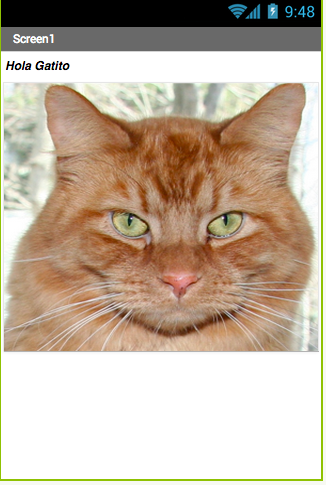
\includegraphics[scale=0.3]{HolaGatito}
  \caption{Pantalla de aplicación \appName{Hola Gatito}}
  \label{fig:holaGatito}
\end{figure}

\subsection*{Qué Aprenderás}

Siguiendo este tutorial aprenderás a:

\begin{itemize}

\item Construir aplicaciones en \AppInventor seleccionando componentes y diciéndoles qué hacer y cuándo hacerlo.

\item Usar el \componentDesigner para seleccionar componentes. Algunos componentes son visibles en la pantalla del dispositivo mientras que otros no lo son.

\item Agregar archivos multimedia (sonidos e imágenes) a las aplicaciones, subiéndoles a \AppInventor desde tu computador.

\item A usar el \blockEditor para ensamblar bloques de código que definen el comportamiento de los componentes, y que por lo tanto en conjunto definen el comportamiento de la aplicación.

\item Probar las aplicaciones directamente en los dispositivos, lo que te ayudará a ver cómo las aplicaciones se comportan, paso a paso, a medida que las construyes.

\item Empaquetar las aplicaciones que construyes para instalarlas en un dispositivo.

\end{itemize}

\subsection*{El Ambiente de Desarrollo \AppInventor}

Para comenzar a programar con App Inventor debes acceder al sitio \aiurl.\footnote{Necesitas una cuenta de Google para utilizar \AppInventor} Esto abrirá la última versión de App Inventor, publicada en Diciembre de 2013. Algunas personas llaman a esta aplicación App Inventor 2, pero su nombre formal sigue siendo App Inventor, y la versión anterior se conoce como App Inventor Classic. Nosotros usaremos siempre la nueva versión.  El entorno de programación App Inventor tiene 3 partes esenciales:

\begin{itemize}

\item El \componentDesigner, que se muestra en la Figura~\ref{fig:componentDesigner}. Se usa para seleccionar los componentes de la aplicación y especificar sus propiedades.

\item El \blockEditor, que se muestra en la Figura~\ref{fig:blockEditor}. Se usa para especificar cómo se comportan los componentes (por ejemplo, qué pasa cuando se presiona un botón).

\item Un dispositivo Android que te permite ejecutar y probar las aplicaciones a medida que las vas desarrollando. Si no tienes un dispositivo Android disponible, puedes probar las aplicaciones usando el Emulador Android. Como en el taller utilizaremos teléfonos móviles no nos preocuparemos de cómo instalar y usar el emulador (igual puedes consultar a tu tutor cómo hacerlo, si quieres programar en tu casa).

\end{itemize}

\begin{figure}[H]
  \centering
  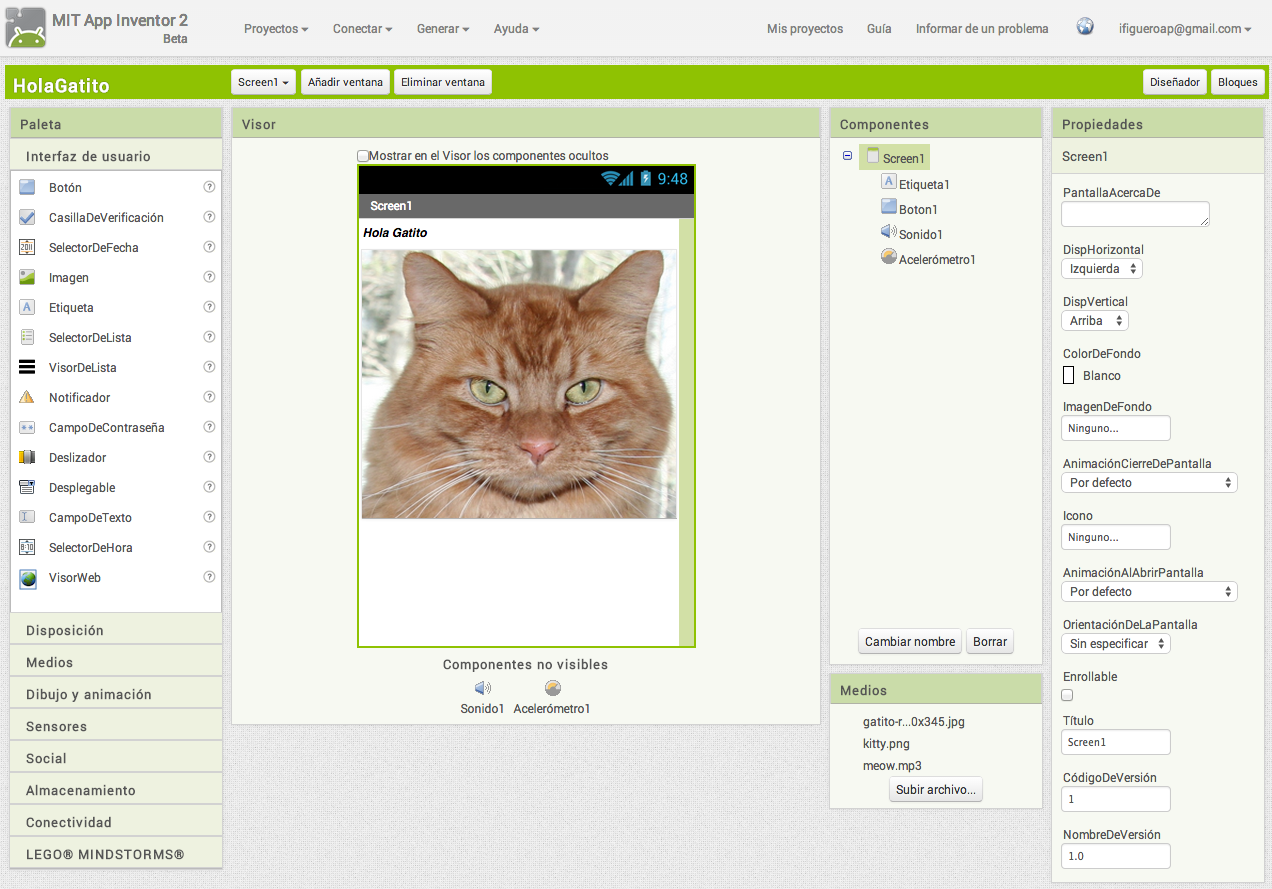
\includegraphics[scale=0.25]{componentDesigner}
  \caption{\componentDesigner}
  \label{fig:componentDesigner}
\end{figure}

\begin{figure}[H]
  \centering
  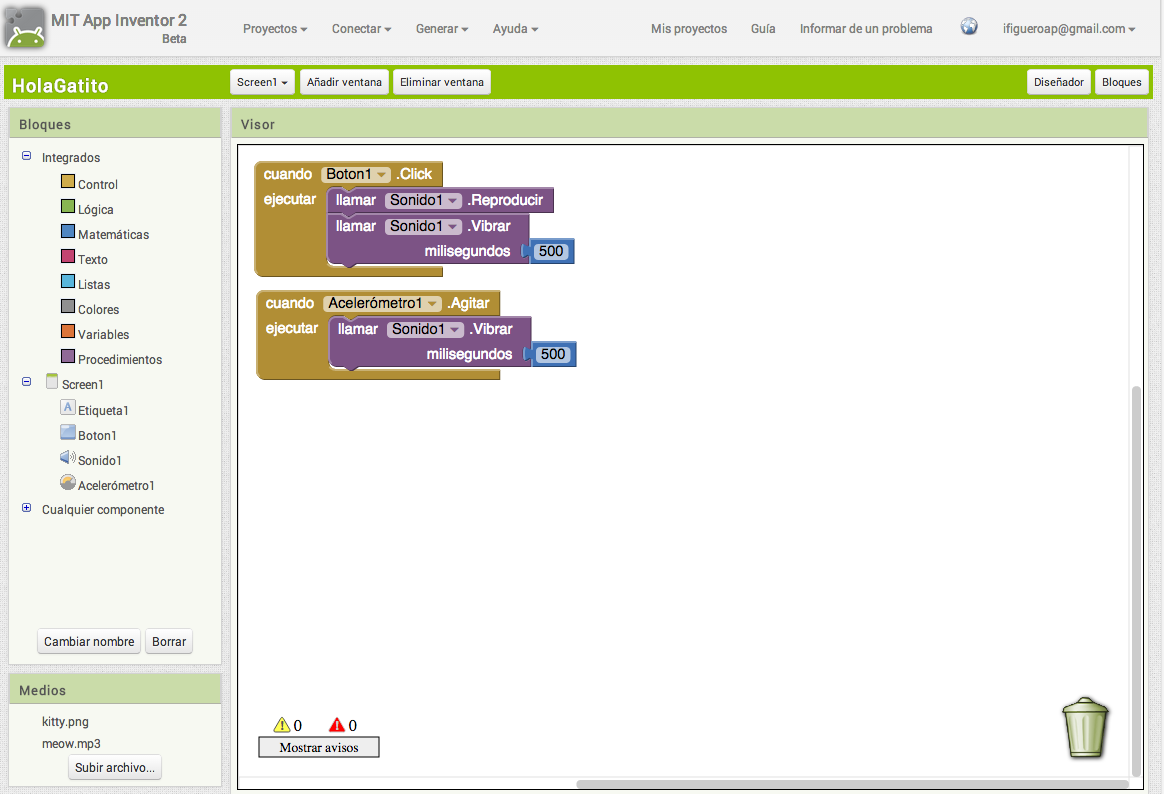
\includegraphics[scale=0.25]{blockEditor}
  \caption{\blockEditor}
  \label{fig:blockEditor}
\end{figure}

La primera vez que ingreses a \aiurl, verás la página de Proyectos, la que seguramente estará en blanco porque aún no has creado ningún proyecto. Para crear un proyecto, presiona el botón ``Comenzar un proyecto nuevo'' en la esquina superior izquierda de la página, ingresa el nombre ``HolaGatito'' (los nombres de proyecto son sin
espacios), y luego presiona ``Aceptar''. LaFigura~\ref{fig:crearProyecto} muestra la creación del proyecto \appName{Hola Gatito}.

\begin{figure}[H]
  \centering
  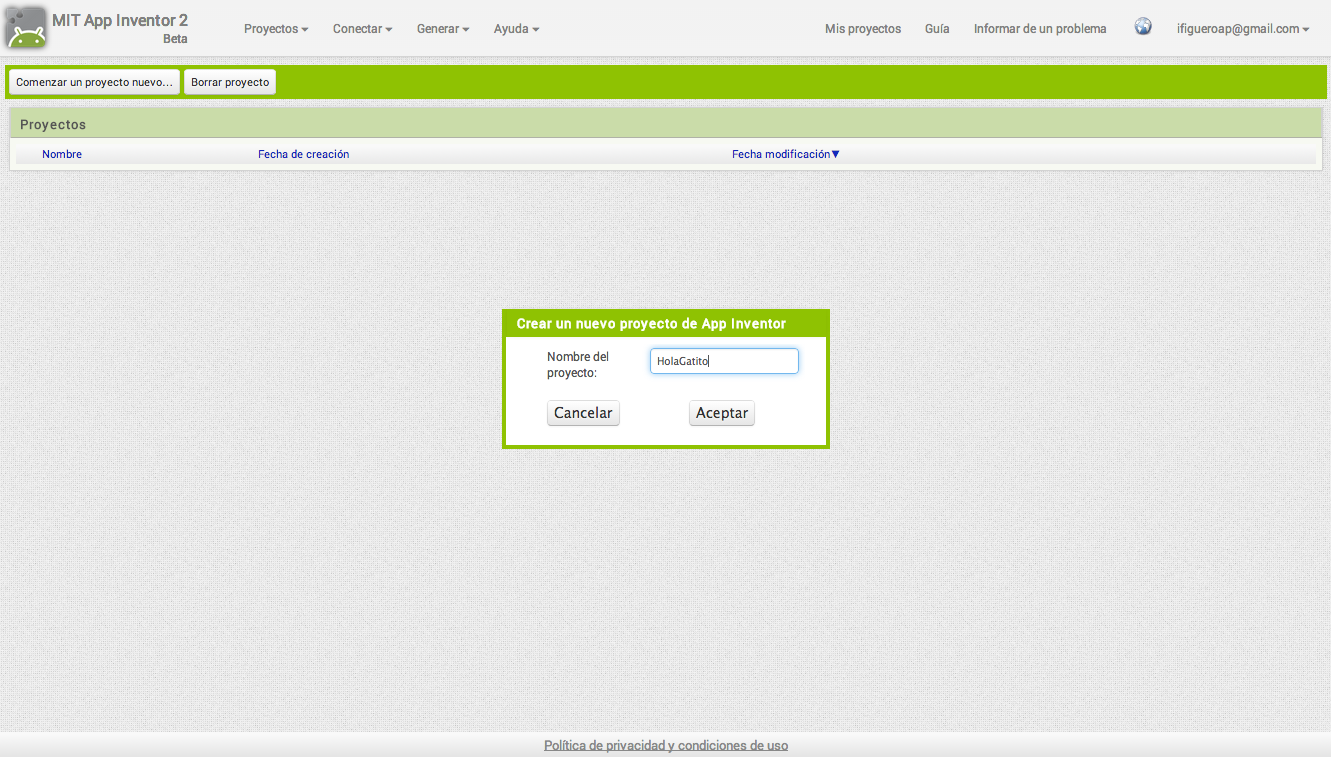
\includegraphics[scale=0.25]{CrearProyecto}
  \caption{Crear proyecto \appName{Hola Gatito}}
  \label{fig:crearProyecto}
\end{figure}

La primera ventana que se abre es el \componentDesigner. El \blockEditor está disponible al hacer click en el botón ``Bloques'' en la esquina superior derecha de la ventana.

\AppInventor es una herramienta computacional \emph{en la nube}, lo que significa que tu aplicación está almacenada en un servidor en línea mientras tú trabajas. Por lo tanto si cierras \AppInventor, tu aplicación estará ahí cuando regreses; no necesitas guardar nada en tu computador, como cuando trabajas con archivos de Word.

\subsection*{Diseñando los Componentes}

La primera herramienta que utilizarás es el \componentDesigner (o simplemente \designer). Los componentes son los elementos que combinas para crear aplicaciones, parecido a los ingredientes de una receta. Algunos componentes son muy simples, como una \component{Etiqueta}, la cual muestra texto en la pantalla, o un \component{Botón}, el cual presionas para iniciar una acción. Otros componentes son más elaborados: un \component{Lienzo} para dibujar, que puede contener imágenes estáticas (sin movimiento) y también animaciones; un \component{Acelerómetro}, que es un sensor de movimiento que funciona de manera parecida a un Wiimote y detecta cuando mueves o agitas el dispositivo. Otros componentes permiten enviar y recibir mensajes de texto (SMS), reproducir música, sonidos, videos, obtener información desde sitios web, etc.

Cuando abras el \designer, éste aparecerá como se muestra en la Figura~\ref{fig:emptyDesigner}

\begin{figure}[H]
  \centering
  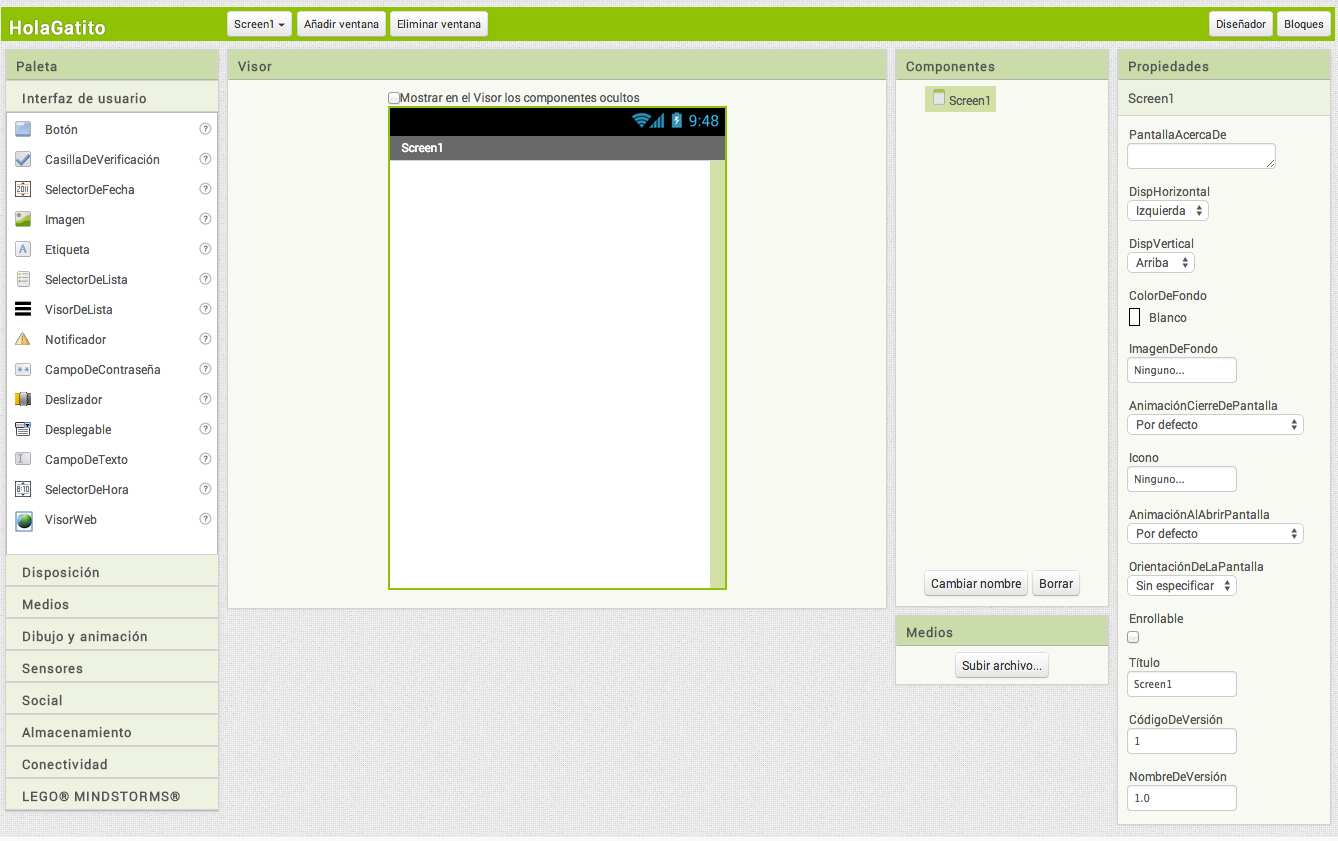
\includegraphics[scale=0.25]{emptyDesigner}
  \caption{El \componentDesigner}
  \label{fig:emptyDesigner}
\end{figure}

El \designer está dividido en varias áreas:

\begin{itemize}

\item En el centro hay un área que se llama \viewer. Aquí es donde tú colocas los componentes y los ordenas para especificar cómo quieres que se vea tu aplicación. El \viewer muestra una aproximación o borrador de cómo se verá la aplicación, por lo que, por ejemplo, una línea de texto podría cortarse en una posición distinta según el dispositivo que uses. Para ver \emph{realmente} cómo se verá una aplicación es necesario probarla directamente en un dispositivo.

\item A la izquierda del \viewer está la \palette, que es una lista de todos los componentes que puedes usar en tu aplicación. La \palette está dividida en secciones. Inicialmente sólo los componentes de la Interfaz de Usuario están visibles, pero basta con hacer click en los nombres de las otras secciones para ver los componentes de cada una de ellas (por ejemplo, Medios, Sensores, etc.).

\item A la derecha del \viewer está la lista de \componentList, que muestra los componentes usados en tu proyecto. Cualquier componente que arrastres en el \viewer también aparecerá en esta lista. Actualmente, el proyecto sólo tiene un componente: \component{Screen1}, que representa la pantalla del dispositivo.

\item Abajo del área \componentList se muestran los \media (imágenes y sonidos) en el proyecto. Este proyecto todavía no tiene ningún archivo multimedia, pero pronto agregarás algunos.

\end{itemize}

Al extremo derecho de la pantalla hay una sección que muestra las \properties de los componentes; cuando seleccionas un componente en el \viewer, verás su lista de \properties en esta sección. Las \properties son detalles sobre cada componente que tú puedes cambiar. Por ejemplo, al seleccionar una \component{Etiqueta}, puedes ver propiedades relaconadas al color, texto, tipo de letra, etc. En este momento está mostrando las propiedades de la pantalla, de nombre \component{Screen1}, las que incluyen el color de fondo, imagen de fondo y título, entre otras.

Para la aplicación \appName{Hola Gatito} necesitarás dos componentes \emph{visibles} (puedes pensar sobre este tipo de componentes como aquellos que se pueden ver en la aplicación): la \component{Etiqueta} que muestra el texto ``Hola Gatito'' y un \component{Botón} con una imagen de un gato. También necesitarás un componente de \component{Sonido}, que es \emph{no-visible}, y que sabe cómo reproducir sonidos, tales como el maullido del gato. Además, necesitarás otro componente no-visible, el \component{Acelerómetro}, para detectar cuándo el dispositivo está siendo agitado. Ahora veremos paso a paso cómo construir la aplicación con cada uno de estos componentes.

\subsubsection*{Agregar la Etiqueta}

El primer componente por agregar es una \component{Etiqueta}:

\begin{enumerate}

\item Selecciona la sección ``Interfaz de Usuario'' en la \palette (si es que no está ya abierta), y arrastra una \component{Etiqueta} hacia el \viewer. Luego de hacerlo, verás una forma rectangular en el \viewer con el texto ``Texto para Etiqueta1''.

\item En el área de \properties de la etiqueta, busca la propiedad ``Texto''. Cambía el valor de esta propiedad por el texto ``Hola Gatito'' y luego presiona Enter. Verás que el texto cambia en el \viewer.

\item Cambia el \backgroundColor de la etiqueta haciendo click en la caja, que actualmente dice ``Ninguno'', para seleccionar un color de la lista que aparecerá. Selecciona Azul. También cambia el \textColor de la etiqueta a Amarillo. Finalmente, cambia el \fontSize a 20.

\end{enumerate}

Luego de seguir estos pasos, el \designer debería verse como en la Figura~\ref{fig:holaGatitoStep1}.

\begin{figure}[H]
  \centering
  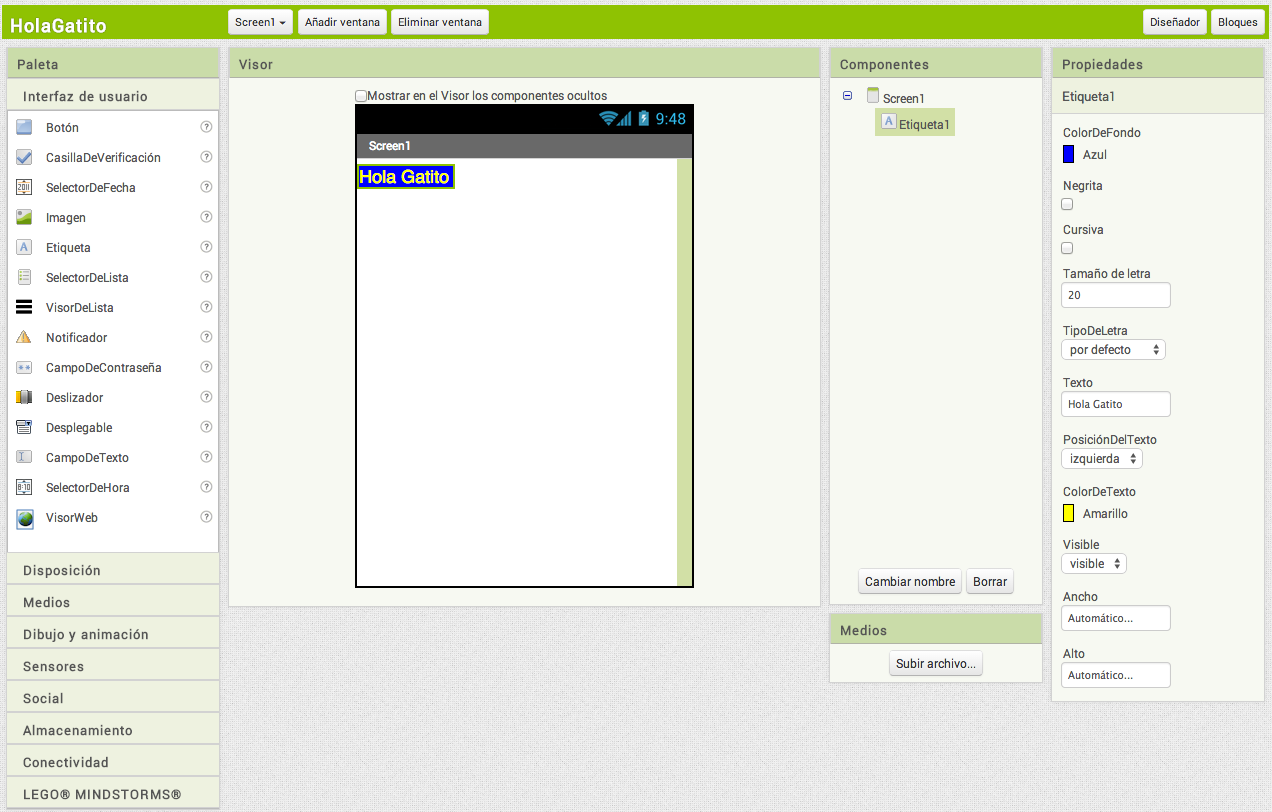
\includegraphics[scale=0.25]{holaGatitoStep1}
  \caption{La aplicación ahora tiene una etiqueta}
  \label{fig:holaGatitoStep1}
\end{figure}

\subsubsection*{Agregar el Bóton}
El gatito para \appName{Hola Gatito} está implementado como un \component{Botón}---creas un botón normal, y luego cambias su imagen de fondo a la del gatito. Para primero agregar un botón normal, debes buscar el componente \component{Botón} en la \palette. Arrastra el botón hacia el \viewer, ubicándolo debajo de la etiqueta. Verás que un botón rectangular aparece en el \viewer.

Ahora tenemos un botón que usaremos para gatillar el efecto de sonido cuando alguien lo presiona, pero lo que realmente queremos es ver la foto de un gatito, y no un simple rectángulo. Para hacer que el botón se vea como la foto del gatito debes hacer lo siguiente:

\begin{enumerate}

\item Primero, necesitas descargar una imagen del gatito y guardarla en tu computador. Puedes descargar la imagen disponible en \resources{ProgramaTusIdeas/Dia1/HolaGatito/gatito.png}. \emph{.png} es una extensión para un formato de archivo estándar, similar a \emph{.jpg} y \emph{.gif}; todos estos formatos pueden ser usados por \AppInventor, así como la mayoría de los formatos de sonido estándar, como \emph{.mpg} o \emph{.mp3}. También puedes descargar el sonido del maullido desde \resources{ProgramaTusIdeas/Dia1/HolaGatito/miau.mp3}. Si quieres, puedes usar tus propias imágenes y sonidos.

\item El área de \properties debería mostrar las propiedades del botón. Si no es así, selecciona el botón en el \viewer para que así sea. En las propiedades del botón presiona el área bajo el teto ``Imagen'' (que actualmente dice ``Ninguno'').

\item Presiona ``Subir archivo'', y luego presiona ``Seleccionar archivo'' para buscar en tu computador el archivo con la foto del gatito (si no usas tu propia imagen, el nombre es \mediafile{gatito.png}). Luego presiona ``Aceptar''.

\item Luego que la imagen se suba, el nombre de archivo debería estar disponible como una opción para la propiedad \property{Imagen} del botón. Presiona ``Aceptar'' para seleccionarla. También verás el archivo listado en el área de \media en la ventana del \designer. Además, en el \designer verás que el botón ahora se ve como la foto del gatito que acabas de seleccionar.

\item Quizás te diste cuenta que la foto del gatito todavía tiene las palabras ``Texto para Botón1''. Probablemente no quieras eso en tu aplicación, por lo tanto borra el texto de la propiedad \property{Texto} para el componente \component{Botón1}.

\end{enumerate}

Ahora el \designer debería verse como en la Figura~\ref{fig:holaGatitoStep2}.

\begin{figure}[H]
  \centering
  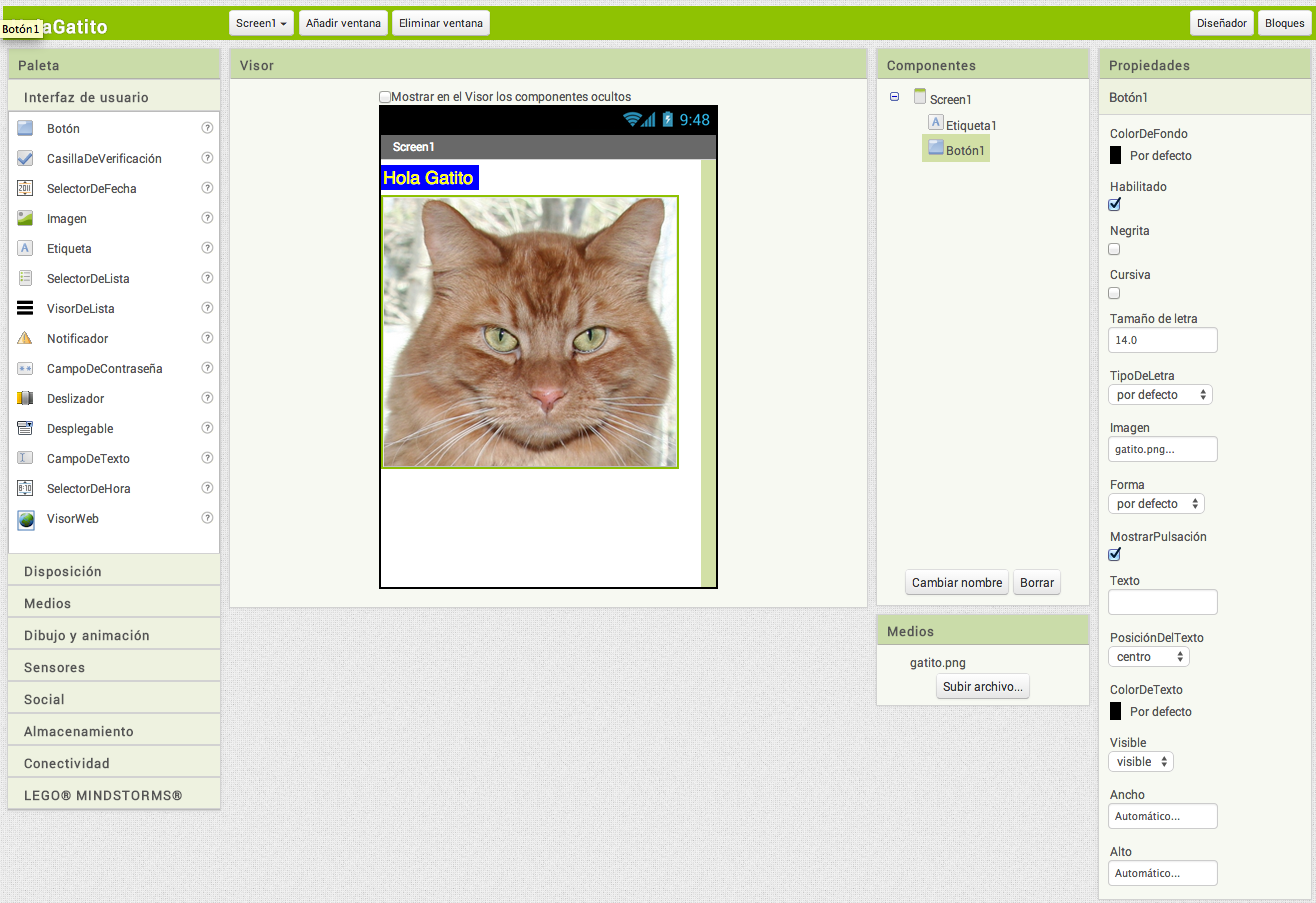
\includegraphics[scale=0.25]{holaGatitoStep2}
  \caption{La aplicación con una etiqueta y un botón con una imagen de un gatito}
  \label{fig:holaGatitoStep2}
\end{figure}

\subsubsection*{Agregar el Maullido}

En tu aplicación quieres que el gatito maulle cuando el botón sea presionado. Para esto, necesitarás agregar el sonido del maullido, y programar el comportamiento del botón para reproducir ese sonido cuando el botón es presionado:

\begin{enumerate}

\item Si aún no has descargado el sonido del maullido, descárgalo ahora desde \resources{ProgramaTusIdeas/Dia1/HolaGatito/miau.mp3}.

\item Ve a la \palette, y selecciona la sección \media. Arrastra un componente \component{Sonido} y cólocalo en el \viewer. Sin importar el lugar donde lo arrastraste, este componente aparecerá en un área abajo del \viewer, llamada ``Componentes no visibles''. Los componentes no visibles son objetos que hacen cosas para la aplicación pero que no aparecen en la interfaz visual del usuario de la aplicación.

\item Selecciona el componente \component{Sonido1} para mostrar sus propiedades. Selecciona su propiedad \property{Origen} y sigue los pasos para subir el archivo \mediafile{miau.mp3} que descargaste anteriormente. Una vez que finalices este paso, deberías ver los archivos \mediafile{gatito.png} y \mediafile{miau.mp3} en el área de \media en el \designer.

\end{enumerate}

La tabla~FOO muestra los componentes que has agregado hasta ahora a la aplicación \appName{Hola Gatito}.

\begin{footnotesize}
  \begin{table}[H]
    \centering
    \begin{tabular}{|p{3cm}|c|c|p{3.5cm}|}
      \hline
      \textbf{Tipo de  Componente} & \textbf{Sección en la \palette} & \textbf{Nombre} & \textbf{Propósito}\\
      \hline
      Botón & Interfaz de usuario & Botón1 & Presionar para que el gato maulle.\\
      \hline
      Etiqueta & Interfaz de usuario & Etiqueta1 & Muestra el texto ``Hola Gatito''.\\
      \hline
      Sonido & Medios & Sonido1 & Reproduce el sonido del maullido.\\
      \hline
    \end{tabular}
    \caption{Componentes que has agregado a la aplicación \appName{Hola Gatito}}
    \label{tab:holaGatitoComponents}
  \end{table}
\end{footnotesize}

\subsection*{Probar la Aplicación}

Con \AppInventor, puedes ver y probar tu aplicación en un dispositivo Android a medida que la vas creando. Probar tu aplicación de manera incremental, paso a paso mientras la desarrollas, es una práctica usada por muchos desarrolladores de software, y que te ahorrará muchas horas de trabajo!

\paragraph{Conexión por puerto USB}
Para conectar las aplicaciones de \AppInventor con tus dispositivos Android usaremos una conexión por cable USB. Esto requiere la instalación de un software especial en tu computador---pero que ya está preinstalado!\footnote{Las instrucciones de instalación, en inglés, están disponibles en \url{http://appinventor.mit.edu/explore/ai2/setup.html}}

Para probar tu aplicación, conecta tu dispositivo al computador usando un cable USB, y luego selecciona la opción ``Conectar'' y específicamente la opción ``USB'', tal como se muestra en la Figura~\ref{fig:conectarUSB}

\begin{figure}[H]
  \centering
  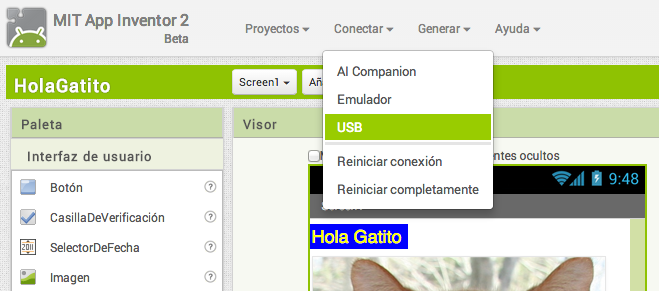
\includegraphics[scale=0.35]{ConectarUSB}
  \caption{Conexión \AppInventor por USB}
  \label{fig:conectarUSB}
\end{figure}

Si todo funciona correctamente, deberías ver la aplicación \appName{Hola Gatito} ejecutándose en tu dispositivo, incluyendo todos los componentes que agregaste. A medida que hagas cambios en el \componentDesigner o en el \blockEditor, estos cambios también aparecerán en el dispositivo. Consulta a tu tutor ante cualquier problema.

Si tu aplicación aparece en el dispositivo, presiona la imagen del gato. ¿Crees que algo pasará? En realidad no pasará nada, porque tu aplicación todavía no le ha dicho al botón qué es lo que debe hacer al ser presionado. Este es el primer punto importante para comprender sobre \AppInventor: para cada componente que agregas en el \designer, tienes que ir hacia el \blockEditor y crear el código para que algo pase con ese componente.

\subsection*{Agregando Comportamiento a los Componentes}

Acabas de agregar componentes de tipo \component{Botón}, \component{Etiqueta} y \component{Sonido} como los bloques con los que construyes tu primera aplicación. Ahora hagamos que el gatito maulle cuando presionas el botón. Esto tienes que hacerlo con el \blockEditor. Presiona el botón ``Bloques'' en la esquina superior derecha del \componentDesigner.

Observa bien la ventana del \blockEditor. Aquí es donde le dices a los componentes qué hacer y cómo hacerlo. Ahora le dirás al botón del gatito que reproduzca un sonido cuando el usuario lo presiona. Si los componentes son los ingredientes en una receta, puedes pensar que los bloques son las instrucciones de cocina.

\subsubsection*{Haciendo Maullar al Gatito}

En la esquina superior izquierda de la ventana, debajo del encabezado ``Bloques'', puedes ver una columna que incluye una sección ``Integrados'', y una sección para cada componente de los que creaste en el \designer: \component{Botón1}, \component{Etiqueta1}, y \component{Sonido1}. Cuando haces click en uno de los componentes, aparecen un montón de opciones (bloques) para ese componente. Presiona el componente \component{Botón1}. Al hacerlo, se muestra una selección de los bloques que puedes usar para decirle al botón qué debe hacer; esta lista comienza con el bloque \block{Botón1.Click}, como se muestra en la Figura~\ref{fig:button1Blocks}.

\begin{figure}[H]
  \centering
  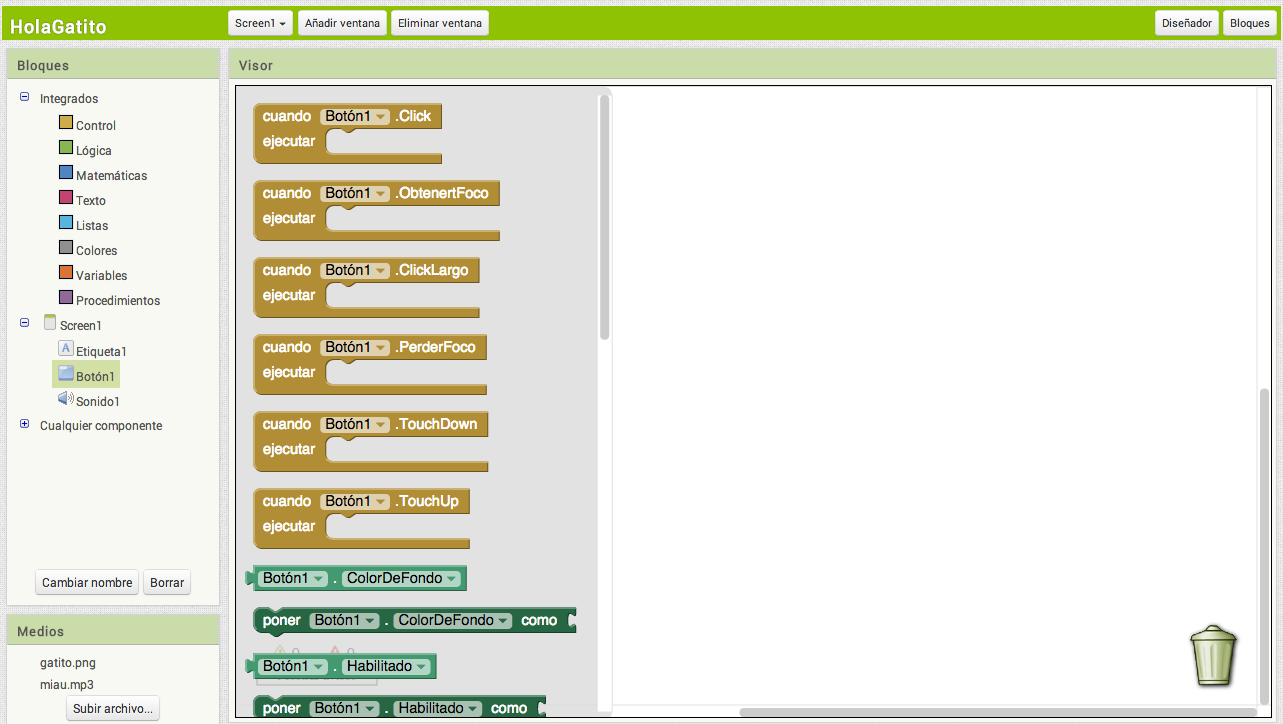
\includegraphics[scale=0.25]{button1Blocks}
  \caption{Al seleccionar el componente \component{Botón1} se muestran sus bloques}
  \label{fig:button1Blocks}
\end{figure}

Arrastra el bloque \block{Botón1.Click} y arrástralo en el \viewer (el espacio en blanco para trabajar con los bloques). Puedes darte cuenta que la palabra \emph{cuando} está incluida en el bloque. Los bloques que incluyen la palabra \emph{cuando} se llaman \emph{controladores de  eventos}. Ellos especifican lo que los componentes deberían hacer \emph{cuando} algun evento particular ocurre. En este caso, estamos interesados en el evento de que un usuario de la aplicación presione el gatito (que en realidad es un botón), tal como se muestra en la Figura~\ref{fig:button1ClickEmpty}. Luego, agregaremos algunos bloques para programar lo que pasará en respuesta a ese evento.

\begin{figure}[H]
  \centering
  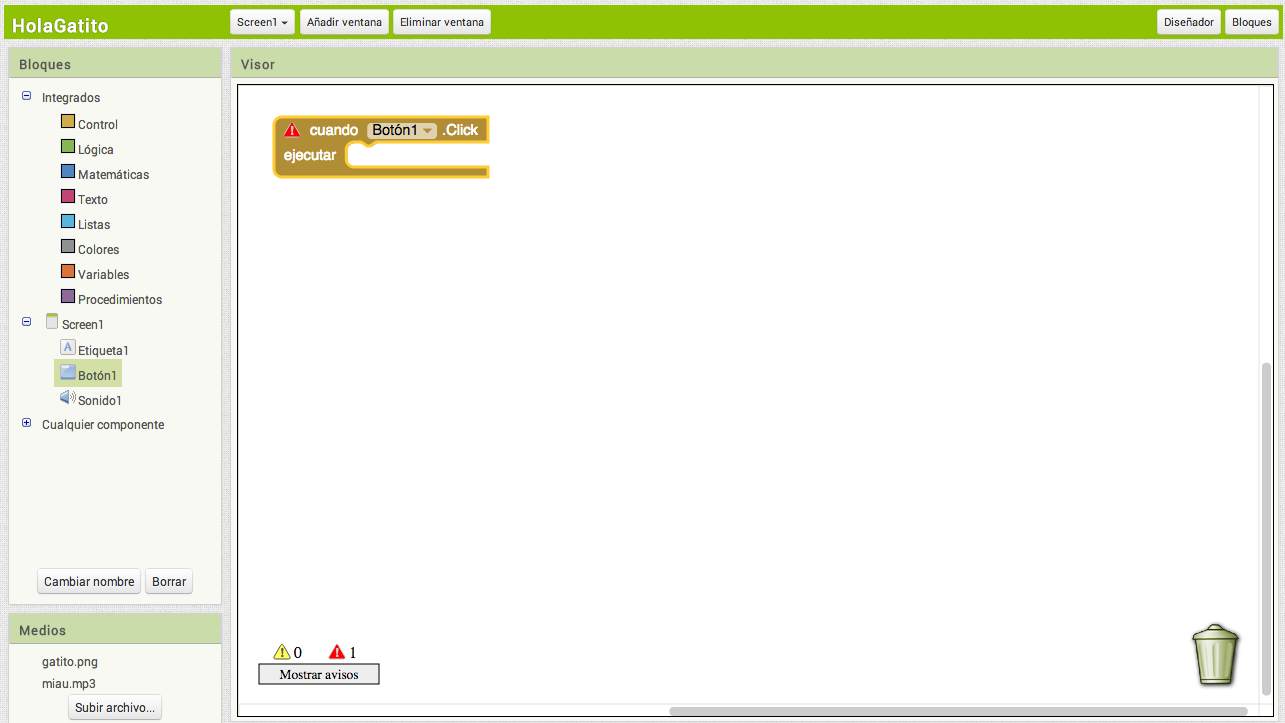
\includegraphics[scale=0.25]{button1ClickEmpty}
  \caption{Especificarás una respuesta al usuario que presiona el botón usando el bloque \block{Boton.Click}}
  \label{fig:button1ClickEmpty}
\end{figure}

Ahora selecciona el componente \component{Sound1} y luego arrastra el bloque \block{llamar Sonido1.Reproducir}. Recuerda que anteriormente configuramos el \property{Origen} del componente con el archivo \mediafile{miau.mp3}. Observa ahora que el bloque \block{llamar Sonido1.Reproducir} tiene una forma tal que es posible ensamblarlo con el espacio marcado como ``ejecutar'' en el bloque \block{Botón1.Click}. \AppInventor está diseñado de manera que sólo ciertos bloques pueden ser ensamblados juntos; de esta manera tu siempre sabrás que estás conectando bloques que en realidad trabajan juntos. En este caso, los bloques con la palabra \emph{llamar} hacen que los componentes hagan cosas. Los dos bloques deben conectarse para formar una sola unidad, como se muestra en la Figura~\ref{fig:button1ClickPlay}. Escucharás un sonido cuando los bloques se conecten correctamente.

\begin{figure}[H]
  \centering
  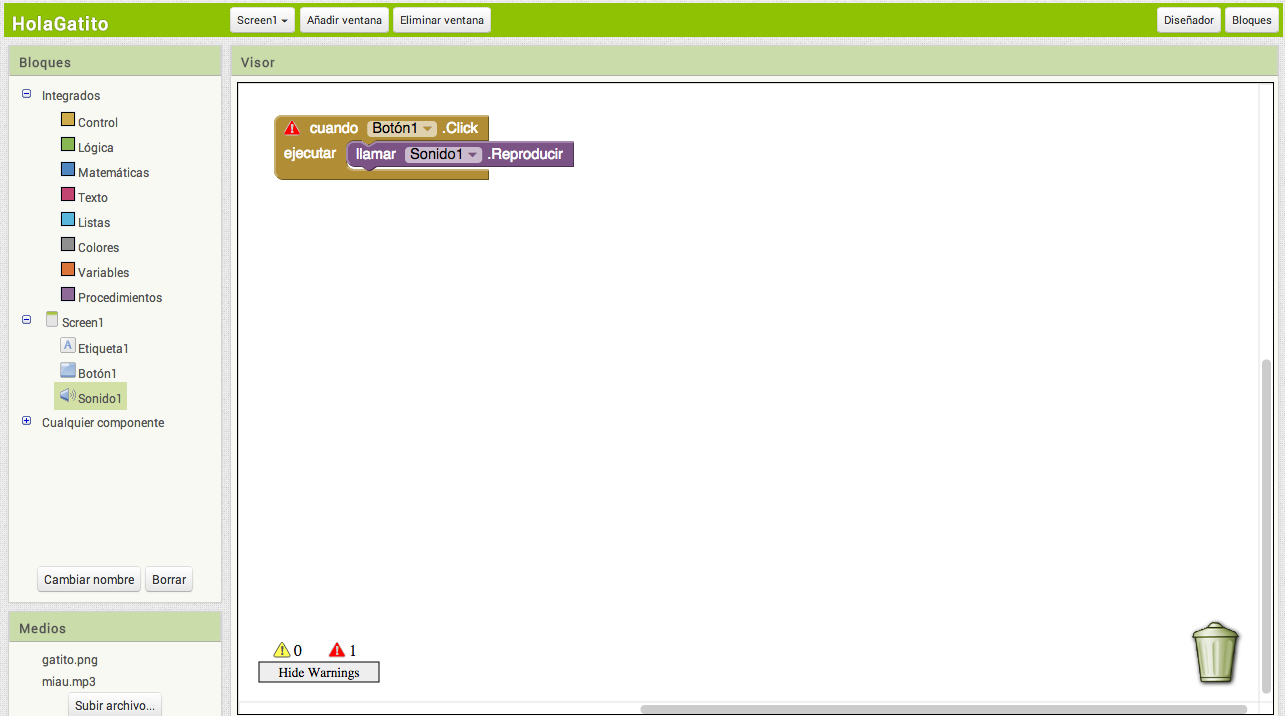
\includegraphics[scale=0.25]{button1ClickPlay}
  \caption{Ahora cuando alguien presione el botón, se escuchará el maullido}
  \label{fig:button1ClickPlay}
\end{figure}

A diferencia del código programado de manera tradicional (el que a menudo se ve como un revoltijo de ``jerigonza''), los bloques de eventos-respuestas en \AppInventor describen los comportamientos que estás intentando crear. En este caso, estamos esencialmente diciendo ``Oye \AppInventor, cuando alguien presione el botón del gatito, reproduce el sonido del maullido''.

\paragraph{Prueba tu Aplicación} Asegúrate que todo esté funcionando correctamente---es importante que pruebes tu aplicación cada vez que agregas algo nuevo. Presiona el botón en el dispositivo. Deberías escuchar el maullido. Felicitaciones, tu primera aplicación se está ejecutando!

\subsubsection*{Agregar el Ronrroneo}
Ahora vamos a hacer que el gato ronrronee y maulle cuando presionas el botón. Simularemos el ronrroneo haciendo vibrar el dispositivo. Eso puede sonar difícil, pero en realidad es muy fácil porque el componente \component{Sonido} que usamos para reproducir el maullido también puede hacer vibrar el dispositivo. \AppInventor te ayuda a aprovechar la funcionalidad esencial de los dispositivos sin tener que preocuparse de \emph{cómo} el dispositivo vibra en la práctica. No necesitas hacer nada nuevo en el \designer, simplemente puedes agregar un nuevo comportamiento al botón en el \blockEditor.

\begin{enumerate}

\item Ve al \blockEditor y selecciona el componente \component{Sonido1}.

\item Selecciona el bloque \block{llamar Sonido1.Vibrar} y arrastralo hacia abajo del bloque \block{llamar Sonido1.Reproducir}. El bloque debería ajustarse en su lugar, como se muestra en la Figura~\ref{fig:button1ClickPlayVibrate}.

  \begin{figure}[H]
    \centering
    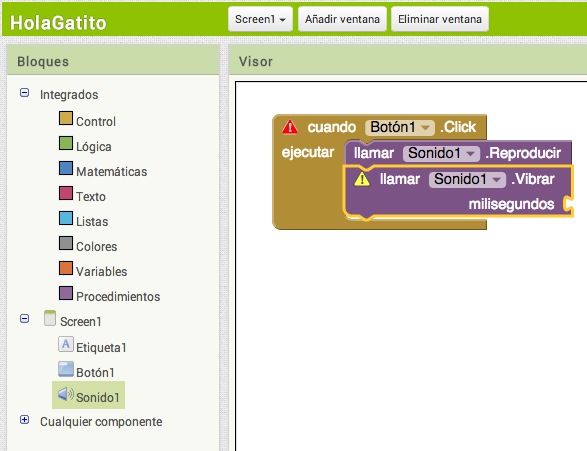
\includegraphics[scale=0.35]{button1ClickPlayVibrate}
    \caption{Reproduciendo el sonido y vibrando en el evento Click}
    \label{fig:button1ClickPlayVibrate}
  \end{figure}


\item Observa ahora que el bloque \block{llamar Sonido1.Vibrar} incluye el texto ``milisegundos''. Un espacio abierto en un bloque significa que necesitas conectar algo ahí para especificar en detalle el comportamiento del bloque. En este caso, debes decirle al bloque por cuánto tiempo debería vibrar. Necesitas agregar esta información en milésimas de segundo (milisegundos), lo que es bastante común en muchos lenguajes de programación. Por lo tanto, para hacer que el dispositivo vibre por medio segundo, tienes que poner un valor de 500 milisegundos. Para poner un valor de 500 necesitas arrastrar un bloque numérico. Selecciona el componente integrado ``Matemáticas'', como se muestra en la Figura~\ref{fig:button1ClickPlayVibrateMillis}. Deberías ver un bloque con un cero como primer elemento. Puedes arrastrar este bloque y cambiar su valor por cualquier otro número.

  \begin{figure}[H]
    \centering
    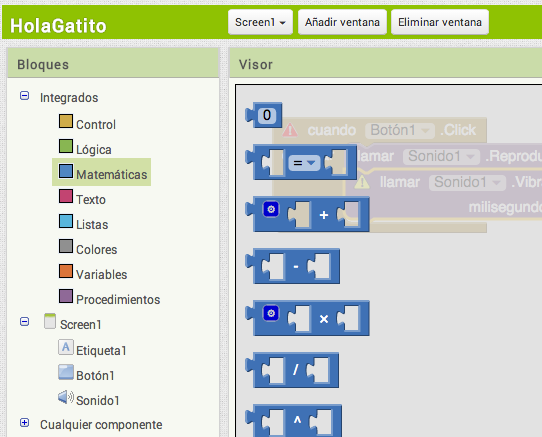
\includegraphics[scale=0.35]{button1ClickPlayVibrateMillis}
    \caption{Agregando un bloque numérico para especificar la duración de la vibración}
    \label{fig:button1ClickPlayVibrateMillis}
  \end{figure}

\item Arrastra el bloque numérico y verás un bloque azul con el número cero, como se muestra en la Figura~\ref{fig:button1ClickPlayVibrateMillis2}.

  \begin{figure}[H]
    \centering
    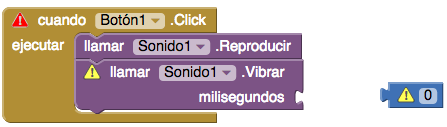
\includegraphics[scale=0.35]{button1ClickPlayVibrateMillis2}
    \caption{Agregando un bloque numérico (0 es el valor por defecto).}
    \label{fig:button1ClickPlayVibrateMillis2}
  \end{figure}

\item Cambia el 0 a 500 haciendo click en el bloque y escribiendo el nuevo valor, como se muestra en la Figura~\ref{fig:button1ClickPlayVibrateMillis3}.

  \begin{figure}[H]
    \centering
    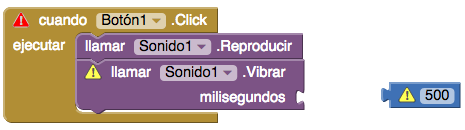
\includegraphics[scale=0.35]{button1ClickPlayVibrateMillis3}
    \caption{Cambiando el valor del bloque numérico a 500.}
    \label{fig:button1ClickPlayVibrateMillis3}
  \end{figure}

\item Conecta el bloque numérico 500 en el espacio del bloque \block{llamar Sonido1.Vibrar}, como se muestra en la Figura~\ref{fig:button1ClickPlayVibrateMillis4}

  \begin{figure}[H]
    \centering
    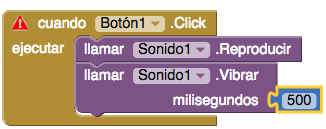
\includegraphics[scale=0.35]{button1ClickPlayVibrateMillis4}
    \caption{Conectando el bloque numérico 500 en el espacio para configurar los milisegundos.}
    \label{fig:button1ClickPlayVibrateMillis4}
  \end{figure}

\end{enumerate}

\paragraph{Prueba tu aplicacion!}

\subsubsection*{Agitando el Dispositivo}

Ahora agreguemos un elemento final que aprovecha otra característica de Android: hacer que el gatito maulle cuando agitas el dispositivo. Para hacer esto, usarás un componente llamado \component{Acelerómetro} que puede sentir cuando agitas o mueves el dispositivo.

\begin{enumerate}

\item En el \designer, expande la sección \sensors en la \palette y arrastra un \component{Acelerómetro} hacia el \viewer. No te preocupes sobre el lugar donde lo arrastrarás, ya que es un componente no visible que aparecerá en la sección justo abajo del \viewer.

\item Vas a querer manejar el que alguien agite el dispositivo como un evento diferente y separado de cuando se presiona el botón. Eso significa que necesitas un nuevo controlador de eventos. Ve al \blockEditor, donde debería haber un nuevo componente \component{Acelerómetro1}. Seleccionalo y arrastra el bloque \block{Acelerómetro1.Agitar}.

\item De la misma forma que lo hiciste con el botón cuando es presionado, arrastra un bloque \block{llamar Sonido1.Reproducir} y conéctalo en el espacio del bloque \block{Acelerómetro1.Agitar}. Los bloques de la aplicación deben quedar como los que se muestran en la Figura~\ref{fig:holaGatitoBlocks}. Prueba tu aplicación agitando el dispositivo!

  \begin{figure}[H]
    \centering
    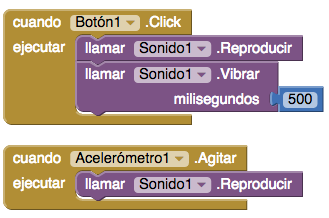
\includegraphics[scale=0.35]{holaGatitoBlocks}
    \caption{Los bloques para la aplicación \appName{Hola Gatito}}
    \label{fig:holaGatitoBlocks}
  \end{figure}

\end{enumerate}

\subsection*{Compartir tu Aplicación}

Puedes compartir tu aplicación de varias maneras. Para compartir la aplicación ejecutable (el archivo .apk que se instala directamente en un dispositivo), primero presiona ``Generar'' y escoge ``App (guardar archivo .apk en mi ordenador''. Esto creará un archivo con una extensión \emph{.apk} en tu computador. Puedes compartir este archivo con otros envíandolo como archivo adjunto en un correo, el cual abrirán con su cliente de correo en el dispositivo donde instalarán la aplicación. También puedes subir el archivo .apk en la web (por ejemplo en DropBox o en tu portafolio). Sólo debes asegurarte que las personas que quieran instalar tu aplicación deben permitir las ``fuentes desconocidas'' en la configuración del dispositivo, para permitir la instalación de aplicaciones que no provienen de la tienda de aplicaciones de Android.

También puedes crear un código QR para tu aplicación de manera que las personas puedan escanear el código en sus dispositivos, desde la web o incluso desde algún poster. Existen numerosas herramientas para crear un código QR desde una URL (por ejemplo, \url{http://qrcode.kaywa.com/}). Una vez que tengas el código QR puedes insertarlo en una página web u otros documentos.

Además, también puedes compartir el \emph{código fuente} (los bloques) de tu aplicación con otro desarrollador que use \AppInventor. Para hacer esto, selecciona ``Mis Proyectos'', elige la aplicación que deseas compartir (en este caso \appName{HolaGatito}), selecciona ``Proyecto'', y luego selecciona ``Exportar a mi ordenador el proyecto (.aia) seleccionado''. El archivo creado en tu computador tendrá extensión \emph{.aia}. Esto le dará a otra persona una copia completa de tu aplicación, la que podrán usar para editar y personalizar sin afectar tu propia versión.

\subsection*{Personalizaciones}

Después que desarrolles las aplicaciones de este taller, seguramente pensarás muchas maneras de mejorarlas. A medida que avancemos con las aplicaciones, también te sugeriremos ideas para que intentes implementarlas. El personalizar las aplicaciones te llevará a explorar los componentes y bloques disponibles, y a aprender a programar por ti mismo sin las instrucciones detalladas que son dadas en los tutoriales. 

Aquí hay algunas ideas para mejorar la aplicación \appName{Hola Gatito}:

\begin{itemize}

\item Mientras agitas el dispositivo, los maullidos sonarán de forma extraña, como si hubiera eco. Esto pasa porque el acelerómetro está gatillando el evento agitar muchas veces por segundo, por lo que los maullidos se solapan. Si te fijas en el componente \component{Sonido} en el \designer, verás una propiedad que se llama \property{IntervaloMinimo}. Esta propiedad determina el tiempo mínimo que hay que esperar para reproducir dos sonidos de forma consecutiva. Actualmente tiene un valor de 400 milisegundos (casi medio segundo), lo que es menor que la duración de un maullido. Jugando con el valor de esta propiedad podrás cambiar la manera en que los maullidos se solapan entre sí.

\item Si exportas la aplicación, la ejecutas, y luego caminas con tu dispositivo en el bolsillo, tu dispositivo maullará cada vez que te muevas bruscamente---algo que quizás pueda ser vergonzoso! Las aplicaciones Android típicamente están diseñadas para seguir ejecutándose incluso cuando no las estas mirando; por lo que tu aplicación sigue comunicándose con el acelerómetro y los maullidos continúan. Para salir realmente de la aplicación, debes mantener presionado el botón de menu en la aplicación \appName{Hola Gatito}. Se te mostrará una opción para cerrar la aplicación, al seleccionarla la aplicación estará completamente cerrada.

  \subsection*{Resumen}

  A continuación repasamos los principales conceptos cubiertos en este tutorial:

  \begin{itemize}

  \item Construyes aplicaciones seleccionando componentes en el \designer y diciéndoles qué hacer y cuándo hacerlo en el \blockEditor.

  \item Algunos componentes son visibles y otros no lo son. Los visibles aparecen en la interfaz de usuario de la aplicación. Los no visibles hacen cosas como reproducir sonidos.

  \item Defines el comportamiento de los componentes juntando bloques en el \blockEditor. Primero arrastras un controlador de eventos como \block{Boton1.Click}, y luego pones bloques de comandos como \block{Sonido1.Reproducir} en su interior. Cualquier bloque contenido dentro de \block{Boton1.Click} será realizado cuando el usuario presione el botón.

  \item Algunos comandos necesitan información extra para hacerlos funcionar. Un ejemplo es \block{Sonido1.Vibrar}, que necesita saber cuántos milisegundos debe vibrar. Estos valores se llaman \emph{argumentos} o \emph{parámetros}.

  \item Los números se representan como bloques numéricos. Puedes conectar estos bloques en comandos que toman números como argumentos.

  \item \AppInventor tiene componentes que representan los sensores del dispositivo. El \component{Acelerómetro} puede detectar cuándo el dispositivo se mueve.

  \item Puedes empaquetar las aplicaciones y descargarlas al teléfono, donde se ejecutan de forma independiente a \AppInventor.

  \end{itemize}

\end{itemize}

\section{Discusión y Personalización}
\label{sec:disc-y-pers}

Para ayudarte a consolidar tus conocimientos sobre \AppInventor te invitamos a responder las siguientes preguntas, y a personalizar tu aplicación siguiendo las sugerencias que se presentan a continuación.

\paragraph{Preguntas}

\begin{enumerate}

\item \AppInventor tiene dos ventanas principales. ¿Cuáles son y qué haces en ellas?

\item Probando e Instalando una Aplicación

  \begin{itemize}

  \item ¿Cómo pruebas una aplicación a medida que la vas desarrollando?

  \item ¿Cómo puedes instalar una aplicación, que tú construiste, en tu dispositivo Android?

  \item ¿Qué pasaría si no tuvieras un teléfono o tablet, pero quisieras programar algunas aplicaciones? ¿Podrías hacerlo? ¿Cómo lo harías?

  \end{itemize}

\item En la aplicación \appName{Hola Gatito} menciona un(a):

  \begin{itemize}
    
  \item componente visible

  \item componente no visible

  \item propiedad

  \item evento

  \item controlador de eventos

  \item llamada a función

  \end{itemize}

\item ¿Qué es un controlador de eventos? ¿De qué está compuesto?

\item Una aplicación consiste de su interfaz de usuario y su comportamiento. ¿En qué consiste el comportamiento de la aplicación?

\end{enumerate}

\paragraph{Ejercicios de Personalización}

\begin{enumerate}

\item Agrega un componente \component{CasillaDeVerificación} que indica si el gatito está durmiendo o no. Si la casilla está chequeada, el gatito duerme, y si no, está despierto.

\item Modifica el comportamiento de la aplicación para tomar en cuenta si el gatito duerme o no. Mientras el gatito duerme, el presionar el botón no emite ningún sonido ni hace vibrar el dispositivo. Si el gatito duerme y se agita el dispositivo, entonces se despierta.

\end{enumerate}


\section{Creando tu Portafolio}
\label{sec:creando-tu-port}

En este tutorial te mostraremos cómo crear tu Portafolio, que incluirá todo el trabajo que realices en el taller. Aprenderás a crear una página en Google Sites, y a partir de este día deberás registrar todo tu trabajo en este portafolio. ¿Por qué vale la pena tener un portafolio? Algunas razones:

\begin{itemize}
\item Estarás creando sobre lo que tus compañeros y amigos pueden aprender.

\item Podrás continuar trabajando en tus proyectos después de que el taller termine.

\item Al tener todo tu trabajo en el portafolio puedes volver a proyectos anteriores a medida que progresas en el taller.

\item Puedes mostrar tu trabajo y progreso a tu familia, tus amigos, que podrán instalar las aplicaciones en sus dispositivos Android.

\item Google Sites es una herramienta que te puede ser útil en el futuro.
\end{itemize}

\paragraph{Google Sites: Tu sitio en la Nube} Utilizamos Google Sites principalmente por las siguientes razones:

\begin{itemize}
\item WYSIWYG (What You See is What You Get): no necesitas saber HTML para editar el sitio.

\item Colaborativo: puedes definir quién edita las páginas. Puedes ser sólo tu, o un grupo, o todo el mundo (como en la Wikipedia).

\item Está almacenado en la Nube: en los servidores de Google. Es difícil que se pierda tu información!

\item Puedes crear un sitio de manera instantánea y crear tantos como quieras, gratis.

\item No necesitas descargar o instalar ningún software en tu computador para modificar tus sitios.
\end{itemize}

\subsection*{Instrucciones}

\begin{enumerate}

\item Para usar Google Sites (y también \AppInventor) necesitas una cuenta de Google. Una vez que tengas la cuenta, abre en tu navegador web la página \url{http://sites.google.com}. Puedes ajustar las preferencias para que el sitio aparezca en Español.

\item Crea un nuevo sitio:

  \begin{itemize}
  \item Presiona el botón ``Crear''.
  \item Ingresa el nombre del sitio, algo como ``Mi Sitio de App Inventor''.
  \item Ajusta o ingresa la ubicación del sitio. Este nombre debe ser único, por lo que puede ocurrir que el nombre que querías ya esté ocupado. 
  \item Escoge la plantilla en blanco. Luego cuando tengas más tiempo puedes cambiar la plantilla y el diseño de tu sitio. Escribe el código de comprobación y luego presiona el botón ``Crear''. LaFigura~\ref{fig:createSite} muestra la interfaz para crear el sitio.

    \begin{figure}[H]
      \centering
      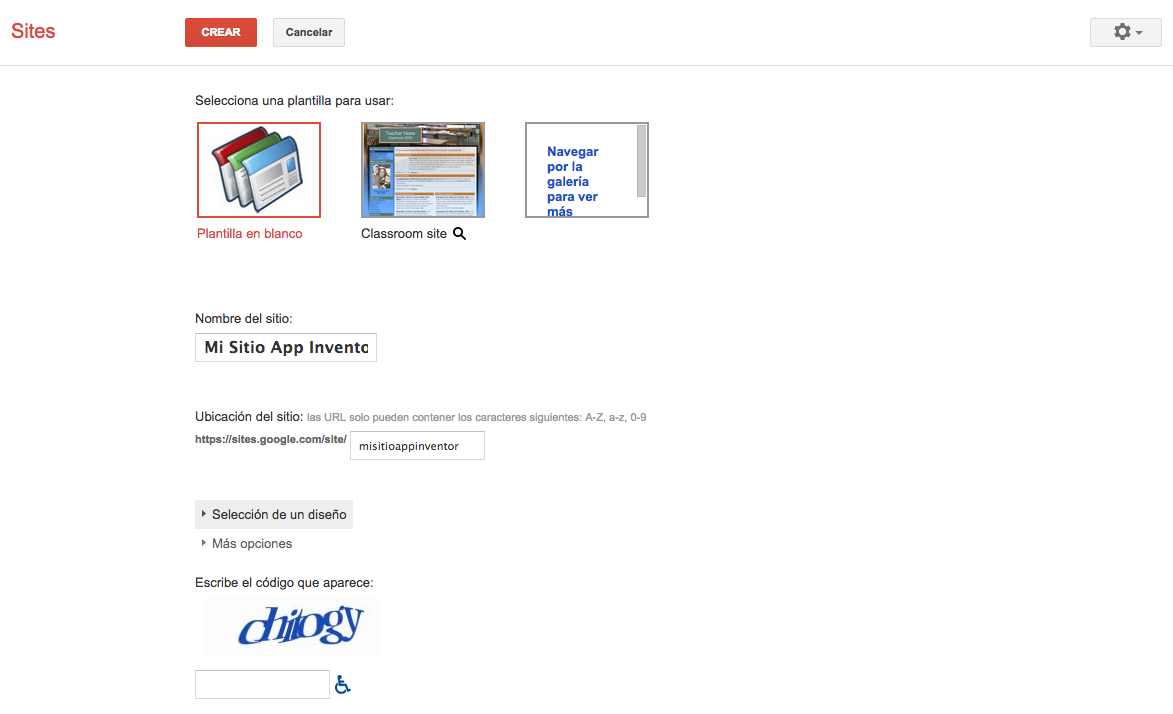
\includegraphics[scale=0.35]{CreateSite}
      \caption{Datos necesarios para crear tu Portafolio en Google Sites.}
      \label{fig:createSite}
    \end{figure}
    
  \end{itemize}

\item Agrega alguna información básica a la página principal, como se muestra en la Figura~\ref{fig:SiteAddInfo}. Para editar la página presiona el botón ``Editar página'', que tiene el ícono de un lápiz, en la esquina superior derecha. Cuando estes en modo de edición, en la misma esquina aparecerán los botones ``Guardar'' y ``Cancelar''. Agrega información tal como:

  \begin{itemize}
  \item nombre e información de contacto
  \item una breve biografía
  \item algún comentario sobre el taller
  \end{itemize}

  \begin{figure}[H]
    \centering
    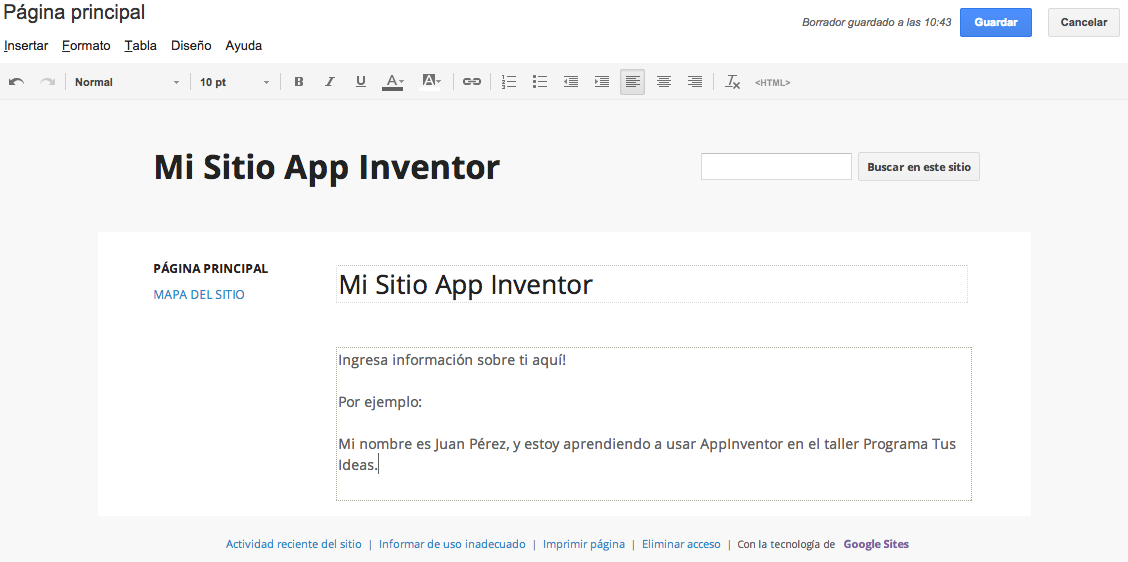
\includegraphics[scale=0.25]{SiteAddInfo}
    \caption{Agregando información básica a tu Portafolio}
    \label{fig:SiteAddInfo}
  \end{figure}

\item Agrega una imagen de perfil a tu página principal. Puedes insertar imágenes ya sea desde tu computador, o desde la Web. Primero inserta una imagen desde la web. Abre otra ventana en tu navegador y busca en Google alguna imagen que quieras usar (ir a \url{http://images.google.com} para buscar imágenes). Cuando encuentras una imagen que te guste, presiona el botón derecho de tu mouse y selecciona la opción ``Copiar URL de imagen'', que pondrá la dirección en el portapapeles. LaFigura~\ref{fig:SiteAddImage2} muestra cómo hacer esto.

  \begin{figure}[H]
    \centering
    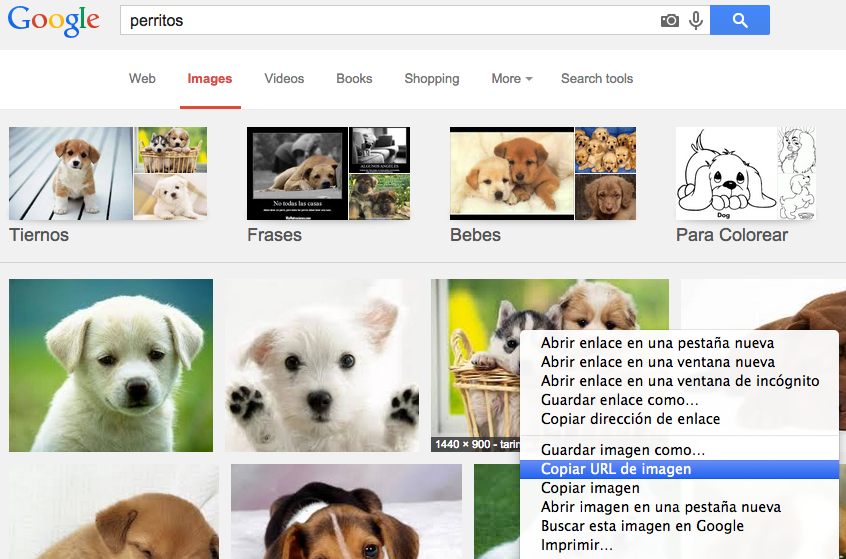
\includegraphics[scale=0.25]{SiteAddImage2}
    \caption{Agregar una imagen desde la web, copiando su URL}
    \label{fig:SiteAddImage2}
  \end{figure}

\item Para poner la imagen en tu sitio, asegúrate de estar en modo de edición y selecciona la opción ``Insertar | Imagen'' en el menú, como se muestra en la Figura~\ref{fig:SiteAddImage1}.

  \begin{figure}[H]
    \centering
    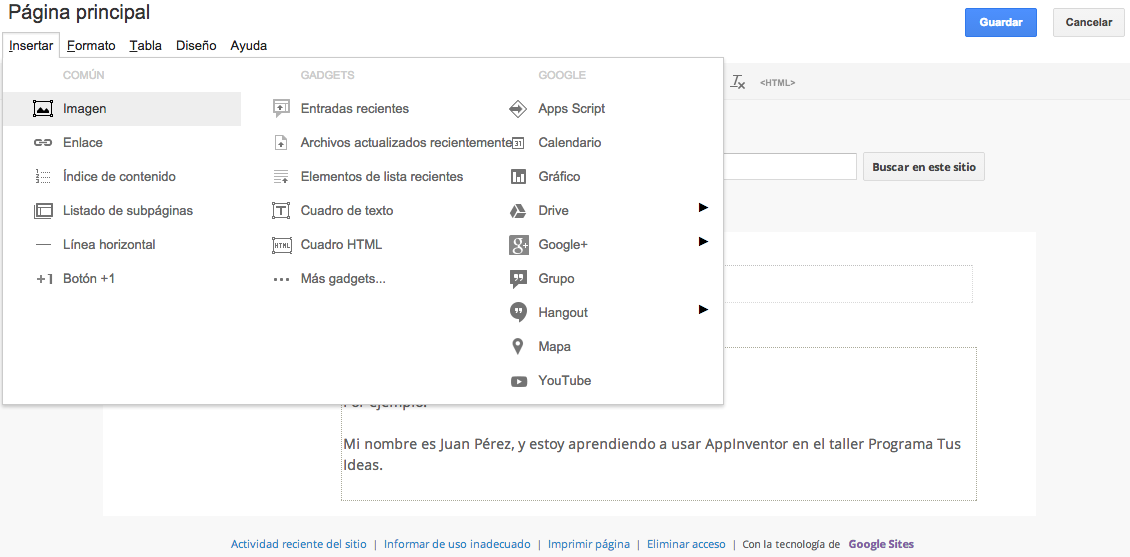
\includegraphics[scale=0.25]{SiteAddImage1}
    \caption{Insertar imagen en tu sitio}
    \label{fig:SiteAddImage1}
  \end{figure}

\item Luego aparecerá una ventana como se muestra en la Figura~\ref{fig:SiteAddImage3}. Selecciona la opción ``Dirección web (URL)'', y pega desde el portapapeles la dirección que copiaste en el paso anterior.

  \begin{figure}[H]
    \centering
    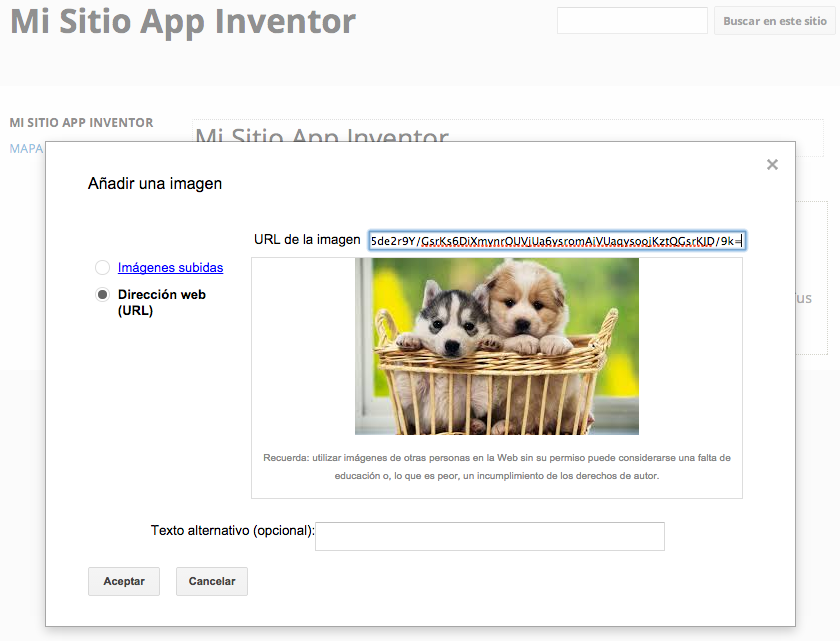
\includegraphics[scale=0.35]{SiteAddImage3}
    \caption{Insertar imagen desde la Web, usando su URL}
    \label{fig:SiteAddImage3}
  \end{figure}

\item También puedes insertar una imagen que esté en tu Para ello debes seleccionar la opción ``Imágenes subidas'' en la ventana del punto anterior, y subir la imagen que desees utilizar.

\item Personaliza el Sidebar (barra lateral) de tu sitio. El sidebar en todos las páginas de tu sitio, y puedes personalizarlo para incluir diferentes elementos y enlaces. Sal del modo de edición y selecciona el botón de opciones (el que tiene un engranaje). Ahí selecciona la opción ``Modificar el diseño del sitio'', tal como se muestra en la Figura~\ref{fig:SiteSidebar1}.

  \begin{figure}[H]
    \centering
    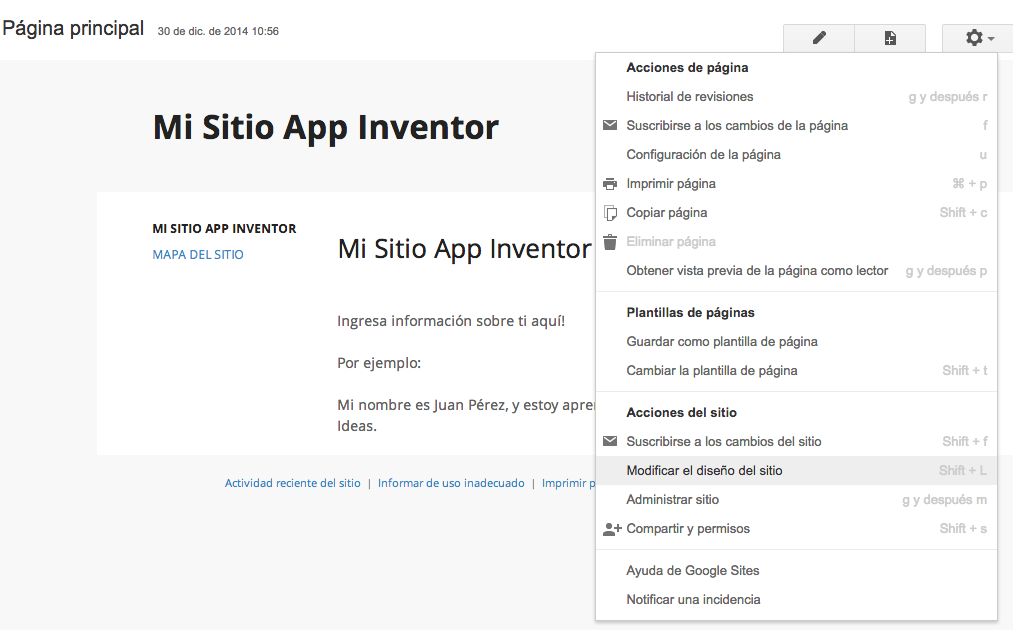
\includegraphics[scale=0.25]{SiteSidebar1}
    \caption{Selecciona la opción para modificar el diseño del sitio}
    \label{fig:SiteSidebar1}
  \end{figure}

\item Ahora la barra lateral estará destacada, y tendrá dos botones: uno para edición (con un lápiz), y uno para agregar elementos (con un signo +). Al agregar un elemento al sidebar, aparecerá una nueva ventana como se muestra en la Figura~\ref{fig:SiteSidebar2}.

  \begin{figure}[H]
    \centering
    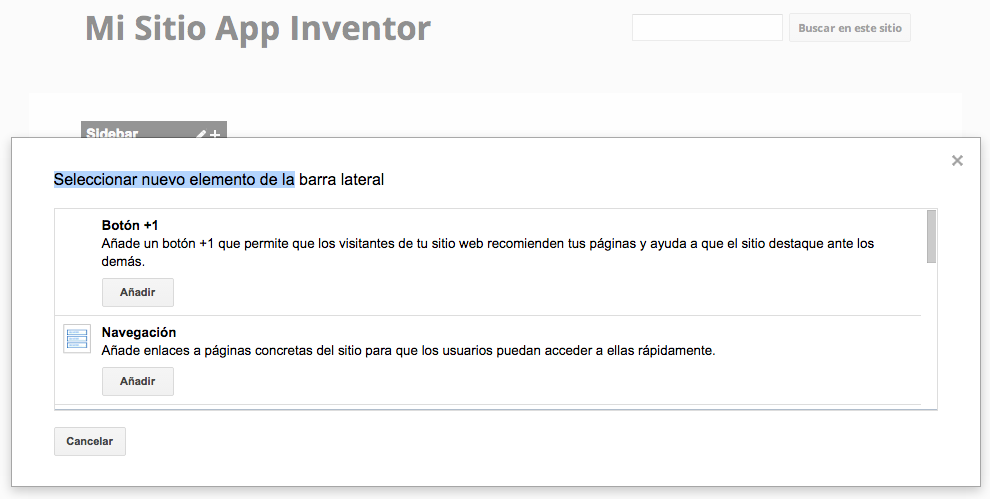
\includegraphics[scale=0.25]{SiteSidebar2}
    \caption{Agregando un nuevo elemento al sidebar}
    \label{fig:SiteSidebar2}
  \end{figure}

\item Para subir archivos a tu sitio, selecciona nuevamente el menú del sitio (como lo hiciste para modificar el diseño del sitio) y escoge la opción ``Administrar sitio''. Entre las opciones que aparecerán escoge ``Archivos adjuntos''. Ahí podras subir, mover y eliminar los archivos que puedes poner a disposición de los visitantes a tu sitio, tal como se muestra en la Figura~\ref{fig:SiteFiles}.

  \begin{figure}[H]
    \centering
    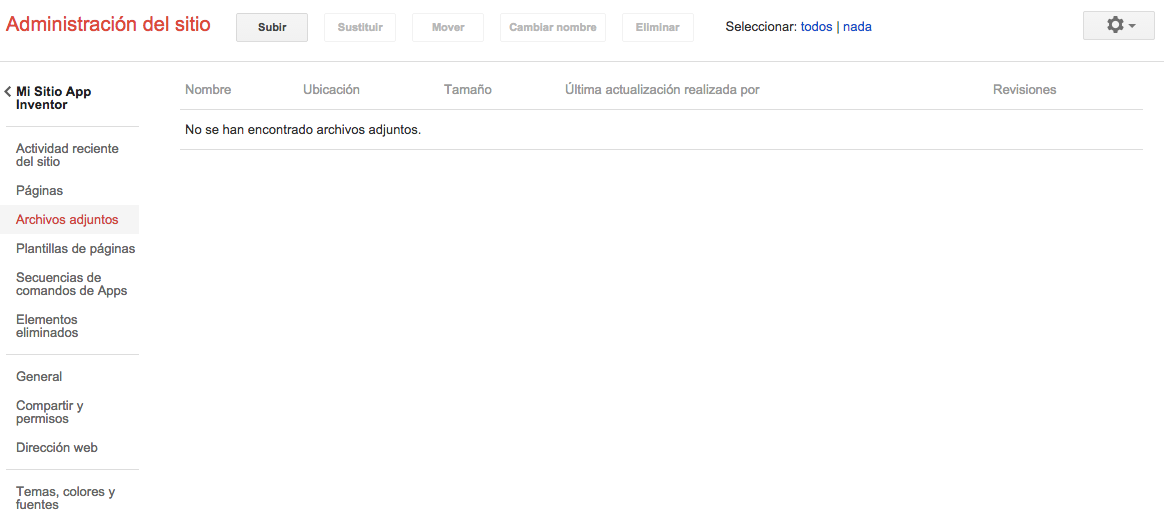
\includegraphics[scale=0.25]{SiteFiles}
    \caption{Administrando los archivos adjuntos de tu sitio}
    \label{fig:SiteFiles}
  \end{figure}



\item Te invitamos a que descubras el potencial de Google Sites para tu portafolio. Recuerda que cualquier duda o problema lo puedes resolver con tu tutor!

\end{enumerate}

\section{Proyecto: Botonera de Sonidos}
\label{sec:proy-boton-de}

La actividad final del primer día de este taller consiste en que realices tu propio proyecto, con un poquito de ayuda inicial. La meta es que desarrolles una aplicación estilo ``botonera de sonidos'', que consiste en múltiples botones que al ser presionados emiten distintos sonidos. Para ayudarte un poco, hemos desarrollado una versión preliminar de la aplicación que puedes descargar desde \resources{ProgramaTusIdeas/Dia1/BotoneraSonidos/BotoneraSonidos.aia}. Luego debes importar este proyecto en \AppInventor.

\paragraph{Interfaz de Usuario}

LaFigura~\ref{fig:botoneraUI} muestra la interfaz de usuario de la aplicación, que consiste en dos botones. A diferencia de \appName{Hola Gatito}, estamos usando un componente de \component{Disposición} para ordenar los botones en la pantalla. Específicamente usamos una \component{DisposiciónTabular} que crea una rejilla donde pueden ponerse otros componentes.

\begin{figure}[H]
  \centering
  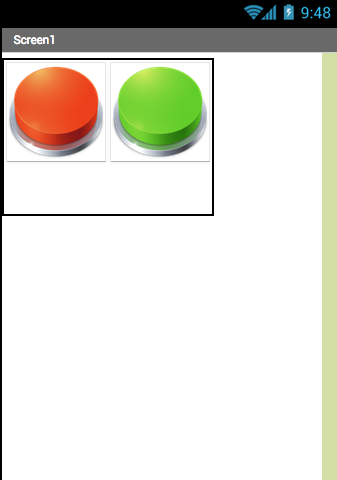
\includegraphics[scale=0.35]{BotoneraUI}
  \caption{Interfaz de usuario de la plantilla para la botonera de sonidos}
  \label{fig:botoneraUI}
\end{figure}

\paragraph{Comportamiento}

El código de la aplicación se muestra en la Figura~\ref{fig:botoneraCode}. El código es muy similar al de \appName{Hola Gatito}, pero tiene una diferencia fundamental. La aplicación tiene sólo 1 componente \component{Sonido}, que se usa para reproducir los sonidos de cada botón. Esto se logra cambiando la propiedad \property{Origen} de forma \emph{dinámica}, dependiendo del botón que es presionado. Para cambiar el origen del sonido, se especifica el nombre del archivo a utilizar (que debe estar subido con anterioridad).

\begin{figure}[H]
  \centering
  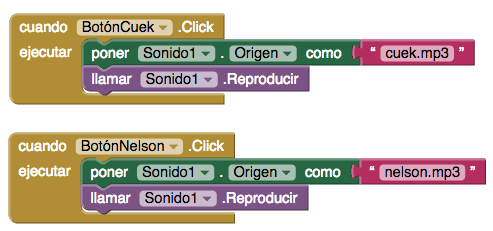
\includegraphics[scale=0.35]{BotoneraCode}
  \caption{Código de la plantilla para la botonera de sonidos}
  \label{fig:botoneraCode}
\end{figure}

\paragraph{Requerimientos del Proyecto}

Puedes crear la aplicación que quieras basándote en la idea y plantilla originales. Sin embargo tu aplicación debiera cumplir al menos los siguientes requerimientos:

\begin{itemize}

\item Debe tener una interfaz de usuario compleja, usando los componentes de \component{Disposición}.

\item Debe tener al menos cuatro sonidos que se reproduzcan en respuesta a distintos eventos (por ejemplo, presionar botones, agitar dispositivo, recibir mensajes de texto, etc.)

\item Debe tener algun comportamiento condicional, usando bloques \block{si, sino}.

\end{itemize}

\paragraph{Ideas} Algunas ideas para ayudarte con tu proyecto:

\begin{itemize}

\item Puedes encontrar y descargar sonidos desde internet, por ejemplo en \url{http://www.myinstants.com/}.

\item Reproducir notas de tus canciones favoritas, discursos, o charlas.

\item Software educacional para niños, por ejemplo una aplicación con los sonidos de una granja.

\item Un juego donde hay que descubrir el nombre de la canción. Al presionar el botón se escucha una parte de la canción, y al presionar otro botón se muestra el nombre de la canción.

\item Una aplicación que hace cosas diferentes cuando recibe mensajes de texto desde otro teléfono.

\item Una aplicación que te permite presionar las fotos de tus compañeros para ver sus nombres y escuchar sus voces.

\end{itemize}

\section{Material de Apoyo}
\label{sec:material-de-apoyo}

\subsection*{Entendiendo la Arquitectura de una Aplicación}

Muchas personas pueden decir qué es lo que es una aplicación, desde la perspectiva del usuario, pero entender qué es una aplicación desde la perspectiva de un \textit{\textbf{programador}} es más complicado. Las aplicaciones tienen una estructura interna, lo que se conoce como la \emph{arquitectura de la aplicación}, que se debe entender para poder crear aplicaciones de manera efectiva.

Una manera de describir el interior de una aplicación es separarla en dos partes: sus \emph{componentes}, y sus \emph{comportamientos}. En general, estos conceptos corresponden a las dos ventanas principales de \AppInventor. Por un lado, se usa el \componentDesigner para especificar los componentes (u objetos) de la aplicación, y por otro lado se usa el \blockEditor para programar cómo la aplicación responde al usuario y a otros eventos externos. O sea, el \blockEditor se usa para programar el comportamiento de la aplicación. LaFigura~\ref{fig:appArchitecture} muestra una vista general de la arquitectura de una aplicación.

\begin{figure}[H]
  \centering
  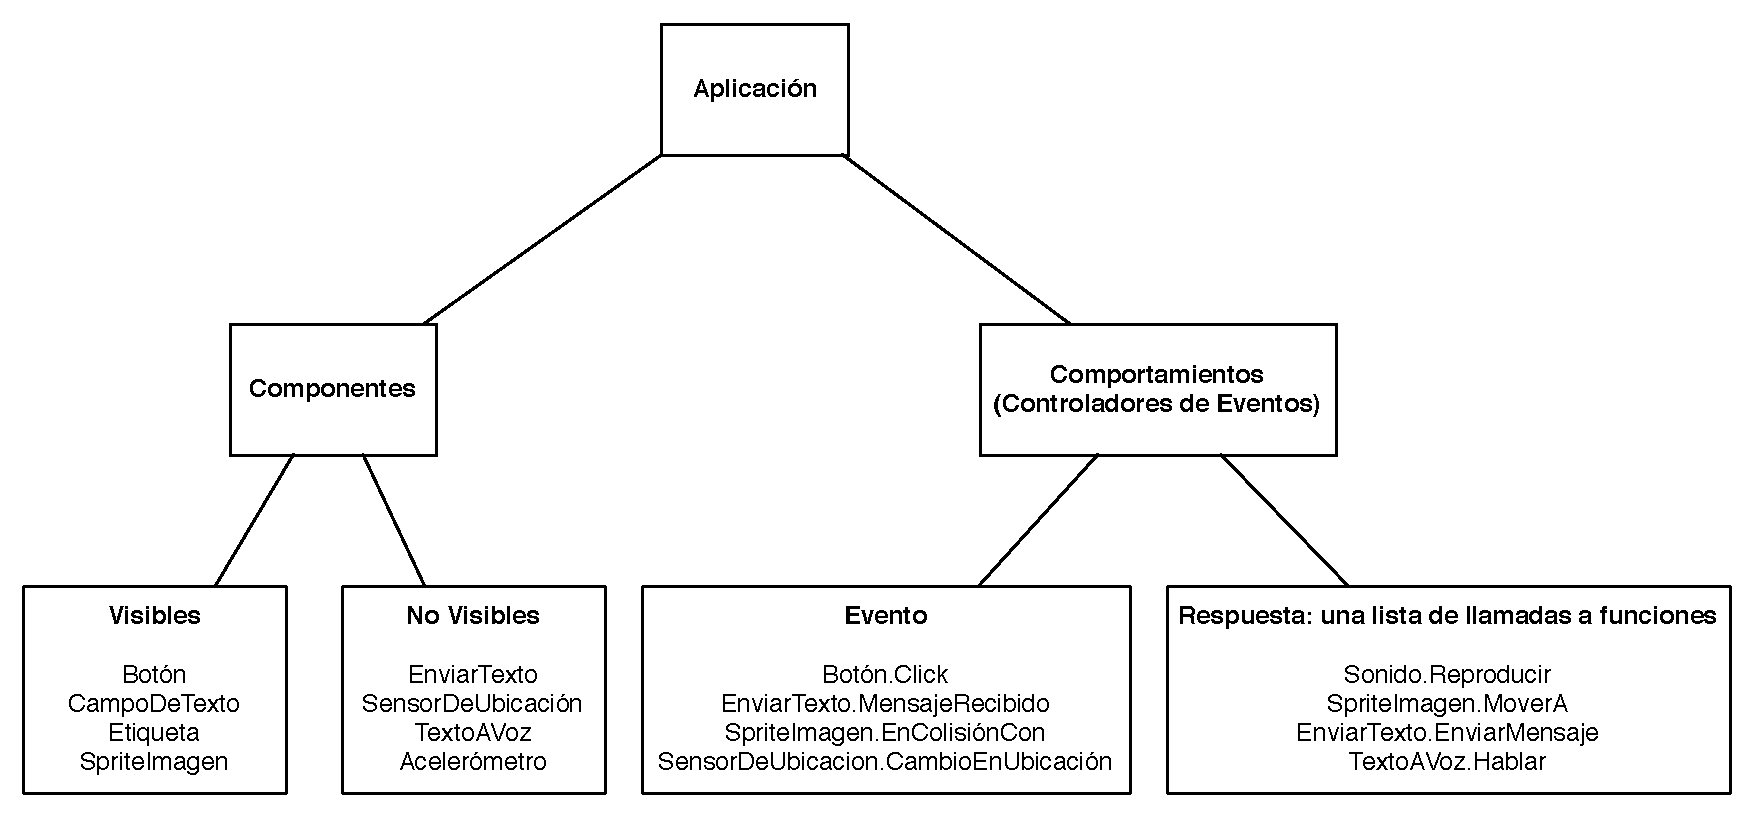
\includegraphics[scale=0.5]{AppArchitecture}
  \caption{Arquitectura de una Aplicación: Componentes y Comportamiento}
  \label{fig:appArchitecture}
\end{figure}

\subsubsection*{Componentes}

Existen dos tipos principales de componentes en una aplicación: \emph{visibles} y \emph{no-visibles}. Los componentes visibles de una aplicación son aquellos que se pueden ver cuando la aplicación se ejecuta, por ejemplo los botones, cajas de texto y etiquetas. Al conjunto de componentes visibles de una aplicación también se le conoce como la \emph{interfaz de usuario}.

Los componentes no-visibles son aquellos que no se pueden ver, y que por lo tanto no son parte de la interfaz de usuario. Su propósito es proveer acceso a las funcionalidad preexistentes de un dispositivo. Por ejemplo, el componente \component{EnviarTexto} envía y procesa los mensajes de texto (SMS), el componente \component{SensorDeUbicación} determina la ubicación del dispositivo, y el componente \component{TextoAVoz} habla un mensaje escrito como texto. Los componentes no-visibles representan la tecnología del dispositivo que está a disposición del programador.

Tanto los componentes visibles como no-visibles se definen por un conjunto de \emph{propiedades}. Las propiedades son espacios de memoria para almacenar información sobre el componente. Los componentes visibles, tales como botones o etiquetas, tienen propiedades como su anchura, altura y alineamiento, los que en conjunto definen cómo luce el componente.
%
Las propiedades de un componente son como celdas de una hoja de cálculo. El programador las modifica en el \componentDesigner para definir la apariencia \emph{inicial} del componente. También es posible utilizar bloques para cambiar estos valores durante la ejecución de la aplicación.

\subsubsection*{Comportamiento}

Los componentes de una aplicación son generalmente sencillos de comprender, por ejemplo un campo de texto se usa para ingresar información o un botón se usa para ser presionado. En cambio, el comportamiento de una aplicación es conceptualmente difícil y a menudo complejo. El comportamiento define cómo la aplicación debiera responder a eventos, tanto eventos iniciados por el usuario (por ejemplo, se presiona un botón) como eventos externos (por ejemplo, se recibió un mensaje de texto). La dificultad de especificar ese comportamiento interactivo es el por qué la programación es un desafío.

Afortunadamente, \AppInventor provee un lenguaje de \emph{bloques} para especificar estos comportamientos. Los bloques hacen que programar el comportamiento sea similar a juntar las piezas de un puzzle, en contraste a recordar y escribir código como en lenguajes de programación tradicionales. Además, \AppInventor está diseñado para especificar comportamientos en respuesta a eventos de una manera sencilla y directa.

\subsubsection*{Una Aplicación es Como una Receta de Cocina}

Tradicionalmente se ha comparado al software (programas, aplicaciones) con una receta de cocina. Como en una receta, una aplicación tradicional sigue una secuencia lineal de instrucciones, como las de la Figura~\ref{fig:lineal}, que el computador debiera ejecutar.

\begin{figure}[H]
  \centering
  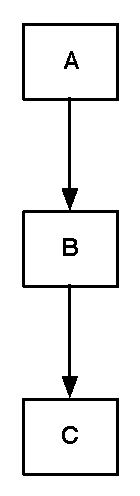
\includegraphics[scale=0.5]{Lineal}
  \caption{Una aplicación tradicional sigue una serie de pasos secuenciales, como una receta de cocina.}
  \label{fig:lineal}
\end{figure}

Si consideramos como ejemplo una aplicación de un cajero automático, una primera operación (A) sería iniciar una transacción bancaria, luego (B) especificar el monto que se desea retirar, y finalmente (C) modificar la cuenta del cliente, entregar el dinero y luego imprimir el saldo por pantalla.

\subsubsection*{Una Aplicación Como un Conjunto de Controladores de
  Eventos}

La visión de una aplicación como una receta de cocina calza bien con las aplicaciones o programas que se hacían en los inicios de la computación, pero no es una gran idea para la programación de dispositivos móviles, ni en la Web, ni en la mayoría de las aplicaciones y plataformas actuales en computación. La mayor parte del software moderno no realiza un puñado de instrucciones en un orden predeterminado. Lo que se hace es que el software \emph{reaccione} ante distintos \emph{eventos}---la mayoría iniciados por la interacción entre el usuario y la aplicación (por ejemplo, abrir un video en Youtube).

En el caso de las aplicaciones móviles tenemos diversos eventos gatillados por el usuario. Por ejemplo, al presionar el botón ``Enviar'', la aplicación responde enviando un mensaje de texto. El deslizar el dedo por la pantalla táctil también es otro evento. La aplicación podría responder dibujando una línea entre el punto donde se comenzó a deslizar el dedo y el punto donde se levantó.

Considerando lo anterior, las aplicaciones modernas se pueden entender mejor como máquinas de eventos-respuestas. Ocurre que las aplicaciones igual incluyen “recetas”—secuencias de instrucciones—pero la diferencia es que cada receta es realizada sólo en respuesta a algún evento en particular. LaFigura~\ref{fig:eventHandlers} ilustra esta idea.

\begin{figure}[H]
  \centering
  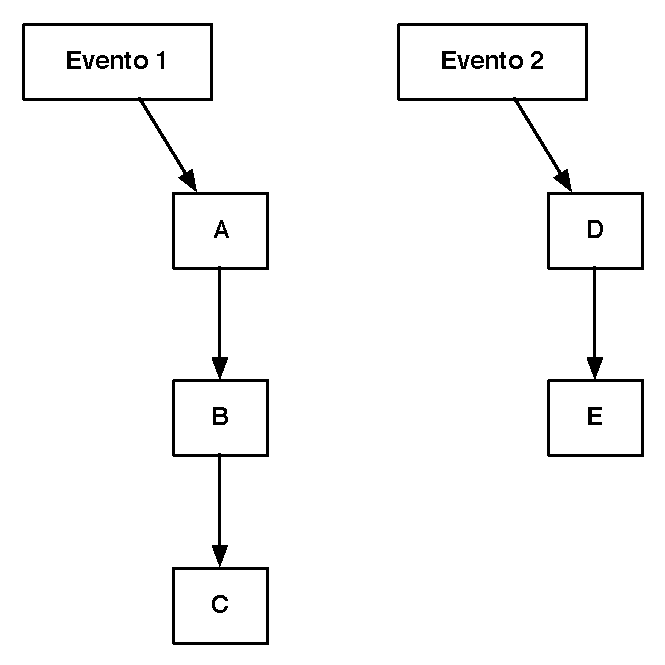
\includegraphics[scale=0.5]{EventHandlers}
  \caption{Una aplicación consiste en un conjunto de controladores de eventos.}
  \label{fig:eventHandlers}
\end{figure}

A medida que los eventos ocurren, la aplicación reacciona ejecutando una secuencia de funciones. Las funciones son cosas que se pueden hacer con un componente (o hacia un componente), como mandar un mensaje de texto o cambiar la propiedad de algún componente (por ejemplo, cambiar el texto de un botón en la interfaz de usuario). \emph{Llamar} a una función significa invocar a esa función, o sea hacer que ocurra lo que esa función hace. Usaremos el término \emph{controlador de eventos} para referirnos tanto a un evento como al conjunto de funciones que se ejecutan como respuesta.

Muchos eventos son iniciados por el usuario, pero algunos no lo son. Una aplicación puede reaccionar a eventos que ocurren al \emph{interior del teléfono}, tales como cambios en su sensor de orientación o su reloj (o sea, respecto al paso del tiempo), y también a eventos creados por cosas \emph{externas al teléfono}, tales como la recepción de un mensaje de texto o una llamada telefónica, o la llegada de datos desde la Web. Esto se muestra en la Figura~\ref{fig:events}.

\begin{figure}[H]
  \centering
  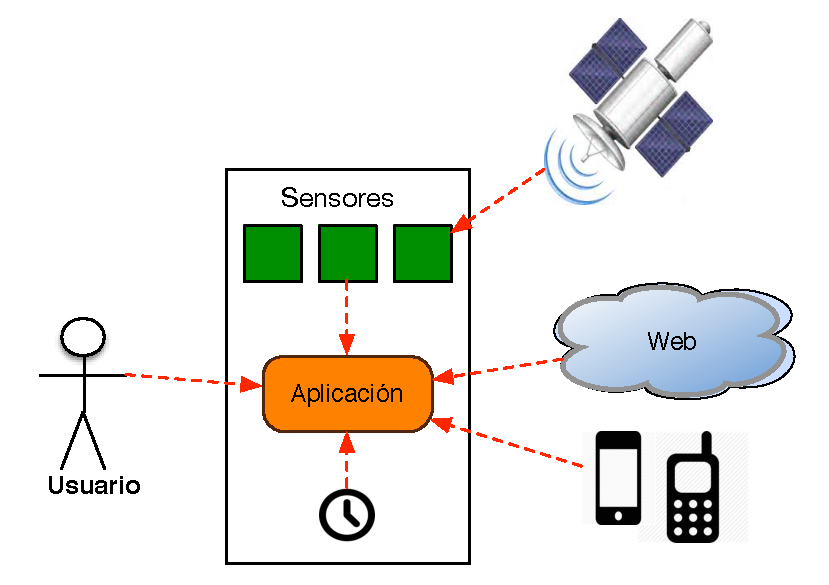
\includegraphics[scale=0.5]{Events}
  \caption{Eventos internos y externos al teléfono.}
  \label{fig:events}
\end{figure}

Una razón por la cual la programación en \AppInventor es intuitiva es porque se basa directamente en este modelo evento-respuesta. Una aplicación se comienza a programar arrastrando un bloque de evento, el cual tiene la forma ``\emph{Cuando} \ldots \emph{ejecutar} \ldots''. Por ejemplo, consideremos una aplicación que responde al evento de presionar un botón leyendo el texto que el usuario a ingresado en una caja de texto, se programa con un único controlador de eventos, como se muestra en la Figura~\ref{fig:speakit1}.

\begin{figure}[H]
  \centering
  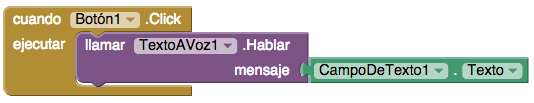
\includegraphics[scale=0.5]{SpeakIt1}
  \caption{Código para hablar texto ingresado por el usuario.}
  \label{fig:speakit1}
\end{figure}

Estos bloques especifican que cuando el usuario presiona el \component{Botón1}, el componente \component{TextoAVoz} debiera hablar las palabras que el usuario ha ingresado en el \component{CampoDeTexto1}. La respuesta al evento \component{Botón1.Click} es la llamada a la función \component{TextoAVoz.Hablar}. El controlador del evento son todos los bloques de la figura.

En \AppInventor, todas las actividades ocurren en respuesta a algún evento. Por lo tanto una aplicación no debiera contener bloques que estén afuera de un bloque “Cuando-ejecutar”. Por ejemplo, no tiene sentido que los bloques de la Figura~\ref{fig:speakit2} estén flotando solos en el editor de bloques.

\begin{figure}[H]
  \centering
  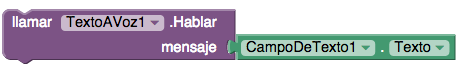
\includegraphics[scale=0.5]{SpeakIt2}
  \caption{Las respuestas deben ir asociadas a un controlador de eventos.}
  \label{fig:speakit2}
\end{figure}

\subsubsection*{Tipos de Eventos}

La Tabla~\ref{tab:eventTypes} resume los tipos de eventos existentes en las aplicaciones \AppInventor. A continuación describiremos cada uno de ellos.

\begin{table}[H]
  \begin{small}
    \begin{tabular}{|l|l|}
      \hline
      \textbf{Tipo de Evento} & \textbf{Ejemplo}\\
      \hline
      Evento iniciado por el usuario & \emph{Cuando} el usuario presiona Botón1, \emph{realizar} ...\\
      \hline
      Evento de inicialización & \emph{Cuando} la aplicación se empieza a ejecutar, \emph{realizar} ...\\
      \hline
      Evento de temporizador & \emph{Cuando} pasen 20 milisegundos, \emph{realizar} ...\\
      \hline
      Evento de animación & \emph{Cuando} dos objetos colisionen, \emph{realizar} ...\\
      \hline
      Evento externo & \emph{Cuando} el teléfono recibe un mensaje de texto, \emph{realizar} ...\\
      \hline
    \end{tabular}
  \end{small}
  \caption{Tipos de Eventos}
  \label{fig:eventTypes}
\end{table}

\paragraph{Eventos iniciados por el usuario} Los eventos iniciados por el usuario son el tipo de evento más común. Con aplicaciones tipo ``trivia'', el presionar botones es la manera usual de gatillar respuestas de la aplicación. Otras aplicaciones más gráficas responden a toques en la pantalla y a arrastrar elementos por la misma.

\paragraph{Eventos de inicialización}
Algunas veces una aplicación necesita realizar ciertas funciones justo cuando la aplicación comienza, y no en respuesta a alguna actividad del usuario final. Para este propósito, \AppInventor considera el ``lanzar'' la aplicación como un evento. Por lo tanto, si el programador lo requiere, se pueden especificar funciones para ser ejecutadas inmediatamente una vez que la aplicación se abre. Para ello se utiliza el bloque \component{Screen1.Inicializar}. En el juego \emph{Atrapa el Topo}, que se realizará el segundo día se utilizará este evento para asignar una posición inicial al azar a un elemento del juego, de forma similar al código de la Figura~\ref{fig:initialize}.

\begin{figure}[H]
  \centering
  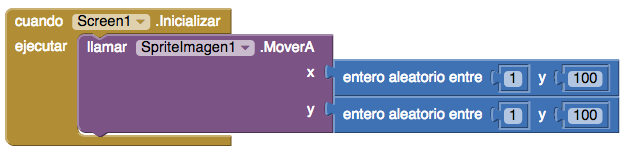
\includegraphics[scale=0.5]{Initialize}
  \caption{Asignando una posición al azar al inicio de la aplicación.}
  \label{fig:initialize}
\end{figure}

\paragraph{Eventos de temporizador}
Algunas actividades de una aplicación son gatilladas por el paso del tiempo. Por ejemplo, uno puede considerar que una animación es un objeto que se mueve gatillado por un evento de temporizador. \AppInventor tiene un componente \component{Reloj} que se usa para gatillar eventos de temporizador. Por ejemplo, el código para mover una pelota por la pantalla 10 pixeles horizontalmente cada cierto intervalo de tiempo es similar al de la Figura~\ref{fig:clockEvent}.

\begin{figure}[H]
  \centering
  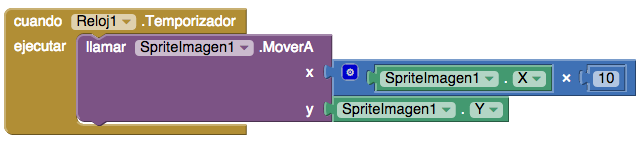
\includegraphics[scale=0.5]{ClockEvent}
  \caption{Animación gatillada por el reloj.}
  \label{fig:clockEvent}
\end{figure}

\paragraph{Eventos de animación}
Las actividades que involucran objetos gráficos (sprites) dentro de lienzos gatillarán eventos. Por lo tanto es posible programar juegos y otras aplicaciones interactivas especificando qué debiera ocurrir en eventos tales como un objeto alcanzando el borde del lienzo, o la colisión de dos objetos. Un código de ejemplo de colisión se muestra en la Figura~\ref{fig:colision}.

\begin{figure}[H]
  \centering
  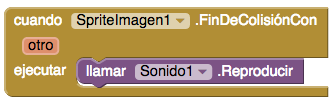
\includegraphics[scale=0.5]{Colision}
  \caption{Controlador de eventos para la colisión entre dos objetos de un juego.}
  \label{fig:colision}
\end{figure}

\paragraph{Eventos externos}

Cuando el teléfono recibe información GPS sobre su ubicación también se gatilla un evento. Lo mismo pasa cuando el teléfono recibe un mensaje de texto, por ejemplo, el código para una respuesta automática a un mensaje de texto recibido se muestra en la Figura~\ref{fig:autoreply}.

\begin{figure}[H]
  \centering
  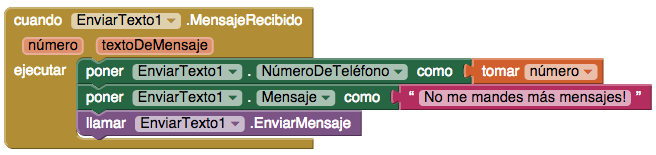
\includegraphics[scale=0.5]{AutoReply}
  \caption{Respuesta automática a un mensaje de texto.}
  \label{fig:autoreply}
\end{figure}

Todos los tipos de eventos se consideran de la misma forma que cualquier otro. En conclusión, cada aplicación creada usando \AppInventor consiste en un conjunto de controladores de eventos: algunos para inicializar cosas, otros para responder al usuario, otros gatillados por el tiempo, y otros gatillados por eventos externos. Tu trabajo como programador es conceptualizar tu aplicación de esta manera, y diseñar la respuesta de cada controlador de eventos relevante para tu aplicación.

\subsubsection*{Los Controladores de Eventos pueden Hacer Preguntas}
Las respuestas a los eventos no siempre siguen recetas de cocina secuenciales, sino que es posible hacer preguntas y repetir operaciones. ``Hacer preguntas'' significa consultar los datos almacenados en la aplicación y determinar el curso de acción (o \emph{rama} de acción) dependiendo de las respuestas a estas consultas. En estos casos decimos que la aplicación tiene \emph{ramas condicionales}, como se ilustra en la Figura~\ref{fig:conditionals}.

\begin{figure}[H]
  \centering
  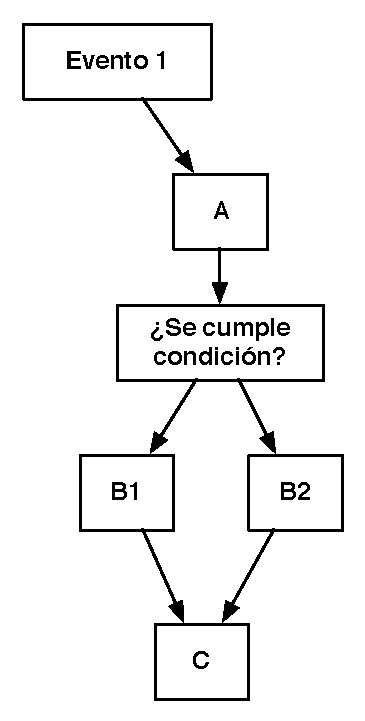
\includegraphics[scale=0.5]{Conditionals}
  \caption{Aplicación con ramas condicionales de ejecución.}
  \label{fig:conditionals}
\end{figure}

Las pruebas condicionales son preguntase tales como ``¿Llegó el puntaje a 100?'', o ``¿El mensaje de texto recién recibido fue enviado por Juan?''.  Las preguntas pueden incluir fórmulas complejas que incluyen comparadores algebraicos (menor que, mayor que, igual a) y lógicos (“y”, “o”, “no”). Los comportamientos condicionales en \AppInventor se especifican usando bloques \block{si, sino}. Por ejemplo, los bloques de la Figura~\ref{fig:score} reportarán el mensaje ``Ganaste!'' si el jugador tiene más de 100 puntos.

\begin{figure}[H]
  \centering
  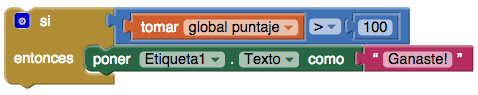
\includegraphics[scale=0.5]{Score}
  \caption{Preguntar si el puntaje es superior a 100.}
  \label{fig:score}
\end{figure}

\subsubsection*{Los Controladores de Eventos pueden Repetir Operaciones}
Además de hacer preguntas y ejecutar distintas recetas según cada caso, una respuesta a un evento puede también incluir repeticiones de operaciones múltiples veces. \AppInventor provee diversos bloques para especificar tales operaciones, tales como \block{por cada} y \block{mientras-comprobar-ejecutar}, los cuales encierran una secuencia de bloques cuya ejecución se repetirá. Todos los bloques dentro de un \block{por cada} se ejecutan una vez para cada elemento en una \emph{lista}. Por ejemplo, el código enviar un mensaje de texto a una lista de números de teléfono es similar al de la Figura~\ref{fig:foreach}.

\begin{figure}[H]
  \centering
  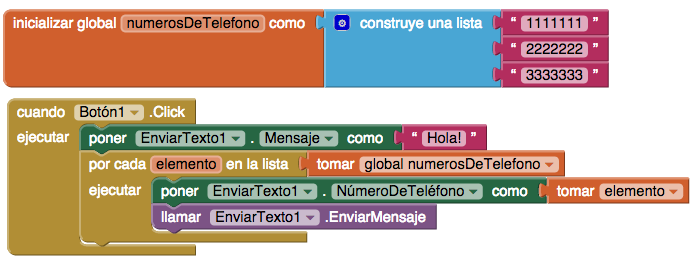
\includegraphics[scale=0.5]{Foreach}
  \caption{Usar repetición para enviar un mensaje de texto a cada teléfono en una lista.}
  \label{fig:foreach}
\end{figure}

\subsubsection*{Los Controladores de Eventos pueden Recordar Cosas}

A menudo un controlador de eventos necesita hacer un seguimiento de la información a medida que ejecuta sus bloques. Esta información puede almacenarse en ubicaciones de memoria conocidas como \emph{variables}, las cuales se definen en el \blockEditor. De hecho, en las secciones anteriores ya hemos visto el uso de variables para almacenar el puntaje de un juego y para definir una lista de números de teléfono.

Las variables son como las propiedades, pero no están asociadas a ningún componente en particular. En un juego, por ejemplo, se puede definir una variable puntaje la cual será modificada por los ontroladores de eventos según la lógica propia de cada juego. Las variables almacenan los datos de manera temporal, mientras la aplicación se está ejecutando; pero cuando se cierra la aplicación los datos dejan de estar disponibles.

A veces una aplicación necesita recordar cosas no sólo mientras se ejecuta, sino incluso cuando es cerrada y vuelta a abrir. Por ejemplo para mantener un historial de los mayores puntajes, es necesario almacenar esta información a largo plazo, de manera que esté disponible la próxima vez que alguien juegue a este juego. Los datos que se mantienen incluso después de que una aplicación se cierra se llaman \emph{datos persistentes}, y se almacenan en algún tipo de base de datos. En los siguientes días del taller profundizaremos más sobre el uso de variables y de datos persistentes.

\end{document}

\newpage
\chapter{Dibujos, Animaciones y Juegos (Parte 1)}
\chapter{Día 2}




%%% Local Variables: ***
%%% mode:latex ***
%%% TeX-master: "Cuaderno.tex"  ***
%%% End: ***
\newpage
\chapter{Dibujos, Animaciones y Juegos (Parte 2)}
\chapter{Día 3}

\section{Animaciones Usando Sprites}

\subsection*{¿Cómo animar Sprites?}

Los componentes \component{SpriteImagen} son objetos especiales que
representan figuras que se mueven por la pantalla. A partir de ahora
los llamaremos simplemente \emph{sprites}. Los sprites están
especialmente diseñados para la creación de animaciones y videojuegos,
y deben utilizarse dentro de un componente \component{Lienzo}. Dentro
de un lienzo, el sprite tiene una \property{Dirección}, una
\property{Velocida} y un \property{Intervalo}. Además, un sprite puede
colisionar con los bordes del lienzo, y con otros
sprites. La~\Cref{fig:spriteMap} cómo se orienta un sprite dentro del
lienzo. La dirección del sprite se representa mediante un ángulo,
entre 0 y 360 grados. El ángulo 0 representa el movimiento hacia la
derecha, y el ángulo 360 hacia la izquierda. Además, los bordes del
lienzo están identificados por números, como se ve en la figura.

\begin{figure}[H]
\centering
\includegraphics[scale=0.5]{spriteMap}
\caption{Configuración del \component{Lienzo} para la animación de Sprites.}
\label{fig:spriteMap}
\end{figure}

\paragraph{¿Cómo reduces la velocidad de un sprite, suavemente, a 100
  pixeles por segundo?}

La velocidad de un \component{SpriteImagen}, que se mide en pixeles
por segundo, es determinada por dos propiedades. La propiedad
\property{Intervalo} especifica cada cuantos milisegundos el sprite se
va a mover, y es muy similar a la propiedad
\component{Reloj.IntervaloDelTemporizador}. La propiedad
\property{Velocidad} específica cuántos pixeles el sprite se moverá en
cada intervalo. En el ejemplo que se muestra en la~\Cref{fig:Sprite1}
el sprite se mueve 5 pixeles cada 50 milisegundos, o 1 píxel cada 10
milisegundos---o sea, 100 pixeles/segundo.

\begin{figure}[H]
\centering
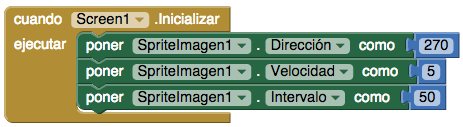
\includegraphics[scale=0.5]{Sprite1}
\caption{Ajustando la dirección, velocidad e intervalo de un sprite.}
\label{fig:Sprite1}
\end{figure}

La propiedad de \property{Dirección} del sprite especifica la
dirección en la cual se mueve. Como se ilustra en
la~\Cref{fig:Sprite1}, el sprite se moverá hacia abajo con una
orientación de 270 grados.

\paragraph{Ejemplo 2: ¿Cómo hacer rebotar una pelota?}

\AppInventor tiene un bloque \block{Botar} que provoca que una pelota
rebote en el borde del lienzo. Típicamente se usa \block{Botar} dentro
del controlador de eventos \block{Pelota.TocarBorde}, dado que este
controlador de eventos indica cual borde ha sido alcanzado, como
parámetro, por lo que puedes conectar este parámetro en la función
\block{Botar}---que necesita saber desde que borde rebotar.

También puedes hacer rebotar otros objetos (sprites o pelotas). El
controlador de eventos \block{EnColisiónCon} se activa cuando dos
objetos chocan. Sin embargo, la función \block{Botar} solamente
funciona en el borde de un lienzo, así que no puede usarse para
colisiones en general. Lo que sí puedes hacer es hacer rebotar el
sprite o pelota en la dirección opuesta a la que tenía antes de la
colisión, configurando su \property{Orientación} como 360 menos el
valor actual. Esto se ilustra en la~\Cref{fig:Sprite2}.

\begin{figure}[H]
\vspace{3em}
\centering
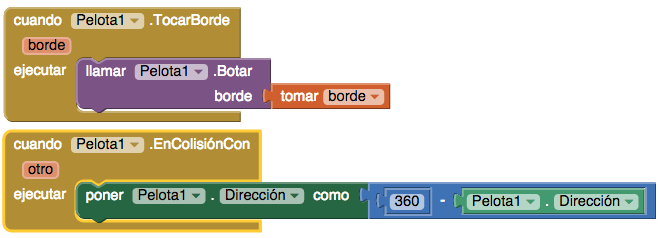
\includegraphics[scale=0.5]{Sprite2}
\caption{Programando una \component{Pelota} para que rebote al tocar
  el borde, y para que invierta su dirección al chocar con otro sprite
u objeto animado.}
\label{fig:Sprite2}
\end{figure}

\subsection*{Desafíos Animados}

\paragraph{Desafío 1: Animación Básica}

Para los siguientes desafíos, necesitarás un componente
\component{Lienzo} que ocupe todo lo ancho de la pantalla y que tenga
unos 300 pixeles de \property{Alto}.  Agrega un botón con texto
``Iniciar!'' abajo del lienzo. Crearás dos aplicaciones distintas:

\begin{enumerate}

\item Mover a la izquierda, abajo y en diagonal usando un
  \component{Reloj}.

  Agregar un componente \component{Reloj} y tres componentes
  \component{Pelota} en el \component{Lienzo}.  Cuando se hace click
  en el botón Iniciar las pelotas deben empezar a moverse dentro del
  lienzo (puedes obtener un movimiento suave al configurar el
  Intervalo de tiempo del \component{Reloj} en 50 milisegundos). Una
  pelota debería ir hacia abajo, otra a la izquierda y otra en
  diagonal. Las pelotas deben parar cuando tocan el borde del
  lienzo. Para este desafío usa sólo 1 componente \component{Reloj} y
  \emph{NO} uses las propiedades de animación internas del componente
  \component{Pelota} (velocidad etc.).

\item Mover a la izquierda, abajo y en diagonal usando una animación
  de Sprite.

  Para este desafío vas a repetir el comportamiento del punto anterior
  pero sin usar un componente \component{Reloj}. En vez de eso,
  utiliza las propiedades de animación internas del componente Pelota:
  \property{Velocidad}, \property{Intervalo} y \property{Dirección}.

\end{enumerate}

\paragraph{Discusión: Velocidad y Cuadros por Segundo}

\begin{enumerate}

\item ¿Qué tan rápido se estaban moviendo tus objetos en el ejercicio
anterior?

\item ¿Cómo determinar la velocidad de tus objetos cuando usas: a) una
  animación Sprite b) un contador de tiempo?. Indica una fórmula para
  cada caso.

\item Los Cuadros por Segundo (CPS) es una medición usada en películas
  y animaciones. Indica cuantas veces por segundo la película se
  actualiza.  ¿Qué CPS se necesita para que el cambio no sea notado
  por el ojo humano?  (Puedes buscarlo en Google)

\item ¿Cuál es el CPS de un juego si el
  \property{IntervaloDelTemporizador} es de 100 milisegundos.

\item Ejercicio de código: modifica uno de tus aplicaciones para que
  un objeto se mueva 50 pixeles por segundo y otro objeto se mueva a
  100 pixeles por segundo.

\end{enumerate}

\paragraph{Desafío 2: Ida y Vuelta }

Crea nuevas aplicaciones para los comportamientos siguientes:

\begin{enumerate}

\item Cuando se presiona un botón, una pelota hace idas y vueltas
  perpetuas en la pantalla.

  \begin{itemize}
  \item Hazlo sin un componente \component{Reloj} (o sea, con una
    animación de Sprite/Pelota).

  \item Hazlo con un componente \component{Reloj}.
  \end{itemize}

\item Cuando se presiona un botón, una pelota se mueve haciendo idas y
  vueltas perpetuas desde el borde izquierdo de la pantalla hasta la
  mitad de la pantalla.

  \begin{itemize}
  \item Hazlo sin un componente \component{Reloj} (o sea, con una
    animación de Sprite/Pelota).

  \item Hazlo con un componente \component{Reloj}.
  \end{itemize}

\end{enumerate}

\section{Tutorial: Pong}

En este tutorial aprenderás a programar una versión sencilla del
clásico juego \appName{Pong}. Hacer este juego te ayudará a
familiarizarte con la animación de sprites, a manejar colisiones, y a
definir procedimientos para que así puedas programar mejor!

A diferencia de los tutoriales anteriores, en este tutorial te
entregaremos un esqueleto de la aplicación, con la interfaz de usuario
ya desarrollada. Tu misión es programar los comportamientos de los
distintos elementos del juego.

La interfaz de usuario final para la aplicación se muestra en
la~\Cref{fig:Pong1}:

\begin{figure}[H]
\vspace{3em}
\centering
\includegraphics[scale=0.5]{Pong1}
\caption{Interfaz de usuario del juego \appName{Pong}}
\label{fig:Pong1}
\end{figure}

Para programar este juego debes seguir los siguientes pasos:

\begin{enumerate}

\item Programa una \component{Pelota} que se mueva en dirección hacia
  abajo. La pelota inicia su movimiento cuando se presiona el botón
  ``Empezar'' (\Cref{fig:Pong2}).

\begin{figure}[H]
\centering
\includegraphics[scale=0.5]{Pong2}
\caption{La pelota se mueve hacia abajo cuando comienza el juego.}
\label{fig:Pong2}
\end{figure}

\item En el programa anterior la pelota es muy predecible, porque
  siempre va en línea recta hacia abajo desde el medio de la
  pantalla. Ahora programa la pelota para que baje en una dirección
  aleatoria---pero que aún es hacia abajo ¿Qué ángulos son ``hacia
  abajo''? (\Cref{fig:Pong3}).

\begin{figure}[H]
\centering
\includegraphics[scale=0.5]{Pong3}
\caption{La pelota se mueve hacia abajo en una dirección aleatoria.}
\label{fig:Pong3}
\end{figure}

\item Programa los rebotes de la pelota: contra los bordes y contra la
  barra.

\begin{figure}[H]
\centering
\includegraphics[scale=0.5]{Pong4}
\caption{La pelota rebota al tocar los bordes y al colisionar con la barra.}
\label{fig:Pong4}
\end{figure}

\item Programa la barra para que se mueva cuando el usuario arrastre
  el dedo. La barra sólo se mueve horizontalmente (o sea, sólo en la
  coordenada X) (\Cref{fig:Pong5}).

\begin{figure}[H]
\centering
\includegraphics[scale=0.5]{Pong5}
\caption{La barra se mueve según el usuario arrastre el dedo sobre ella.}
\label{fig:Pong5}
\end{figure}

\item Modifica el programa para obtener 1 punto cada vez que la barra
  golpea la pelota. Para esto vas a usar un procedimiento con
  argumentos, averigua por ti mismo, o consulta a tu tutor al
  respecto (\Cref{fig:Pong6}).

\begin{figure}[H]
\centering
\includegraphics[scale=0.5]{Pong6}
\caption{Aumentando el puntaje cada vez que se golpea la pelota con la
barra.}
\label{fig:Pong6}
\end{figure}

\item Modifica el programa para que el juego termine si la pelota
  choca con el borde de abajo (\Cref{fig:Pong7}).

\begin{figure}[H]
\centering
\includegraphics[scale=0.5]{Pong7}
\caption{El juego termina cuando la pelota choca con el borde de abajo.}
\label{fig:Pong7}
\end{figure}

\item Agrega un componente \component{Sonido} y modifica el programa para agregar distintos efectos de sonido
  cuando la pelota choca en la barra, toca los bordes, y para el fin
  del juego (los archivos ya vienen incorporados en el proyecto
  inicial, ver~\Cref{fig:Pong8}).

\begin{figure}[H]
\vspace{3em}
\centering
\includegraphics[scale=0.5]{Pong8}
\caption{Efectos de sonido para las colisiones, toque de bordes y fin
  del juego.}
\label{fig:Pong8}
\end{figure}

\item Agrega un component \component{CasillaDeVerificación} para que
  el usuario puede apagar/prender el sonido (\Cref{fig:Pong9}).

\begin{figure}[H]
\centering
\includegraphics[scale=0.5]{Pong9}
\caption{La reproducción de sonidos depende del valor de la casilla de
verificación.}
\label{fig:Pong9}
\end{figure}





\end{enumerate}

\section{Proyecto: Crea tu Propio Juego o Aplicación}

Crea una aplicación con animaciones similares--pero más
complejas---que en el juego \appName{Atrapa el Topo} y \appName{Pong}.

La aplicación debe tener las siguientes funcionalidades:

\begin{itemize}

\item Objetos que se mueven en el tiempo (por ejemplo una nave
  espacial que atraviesa la pantalla).

\item Objetos que se mueven o son transformados en reacción a la
  actividad del usuario (por ejemplo el sensor de orientación para
  controlar el movimiento).

\item Objetos que aparecen o desaparecen en reacción a las actividades
  del usuario (por ejemplo, un asteoride que desaparece cuando recibe
  un disparo).

\item Uso de bloques condicionales.

\item Uso de bloques \block{EnColisiónCon} y \block{TocarBorde}.

\end{itemize}

¡Se creativo! No necesitas crear un juego, puedes crear lo que tu
quieras mientras muestre todos los comportamientos listados arriba.
Comparte tu idea con tu tutor y aseguráte que tienes todos los
comportamientos requeridos.

\section{Material de Apoyo: Variables, o Cómo Programar la Memoria de
tu Aplicación}

Así como las personas necesitan recordar cosas, también las
aplicaciones lo necesitan. En este material de apoyo volveremos al
tema de las variables, pero ahora con mayor profundidad y
detalle. Como vimos anteriormente, la idea esencial de usar variables
es programar una aplicación para que recuerde información.

Cuando alguien te dice el número de teléfono de una pizzería, tu
cerebro lo almacena en una \emph{celda de memoria}. Si alguien
menciona algunos números para que tu los sumes, tu también almacenas
estos números y los resultados intermedios en una celda de memoria. En
estos casos, no estás totalmente conciente de cómo tu cerebro almacena
o recuerda la información.

Una aplicación también tiene memoria, pero su funcionamiento interno
es mucho menos misterioso que el de tu cerebro. Ahora veremos en
detalle cómo manejar la memoria de una aplicación, cómo almacenar
información en ella, y cómo recuperar esa información en un momento
posterior.

\subsection*{Celdas de Memorias Definidas}

La memoria de una aplicación consiste de una serie de celdas de
memoria definidas. Algunas de estas celdas de memoria se crean cuando
arrastras un componente en tu aplicación. Estas celdas (o espacios
abiertos) se llaman \emph{propiedades}. También puedes definir celdas
de memoria definidas que no sean asociadas con un componente
específico. Estas se llaman \emph{variables}. Aunque las propiedades
están típicamente asociadas a lo que es visible en la app, las
variables pueden ser asociadas a la \emph{memoria escondida} de la
aplicación.

\subsection*{Propiedades}

Tú, como usuario de una aplicación, puedes ver componentes visibles
como botones, cuadros de texto y etiquetas. Pero adentro, cada
componente es completamente definido por una serie de propiedades. Los
valores almacenados en la memoria de cada propiedad determina cómo
aparece el componente. Tú configuras los valores de las propiedades
directamente en el Diseñador de Componentes. Por ejemplo,
la~\Cref{fig:Variable1} muestra el panel para modificar las
propiedades de un componente \component{Lienzo}.

\begin{figure}[H]
\centering
\includegraphics[scale=0.5]{Variable1}
\caption{Hoja de propiedades para un componente lienzo.}
\label{fig:Variable1}
\end{figure}

El componente \component{Lienzo} tiene varias propiedades de distintos
tipos. Por ejemplo el \property{ColorDeFondo} y el
\property{ColorDePintura} son celdas de memoria que contienen un
color. La propiedad \property{ImagenDeFondo} contiene un nombre de
archivo (como \mediafile{gatito.png}).

La propiedad \property{Visible} contiene un valor booleano (verdadero
o falso, dependiendo si se selecciona la opción o no). El
\property{Ancho} y \property{Alto} contienen un número o una
designación especial (por ejemplo, ``Ajustar al Contenedor'').

Cuando configuras una propiedad en el \componentDesigner, especificas
el valor inicial de está propiedad, o sea su valor cuando se inicia la
aplicación. Los valores de las propiedades también pueden ser
modificados cuando la aplicación se ejecuta, mediante el uso de
bloques. Pero, al cambiar los valores durante la ejecución, los
valores que aparecen en el \componentDesigner no cambian---estas
propiedades siempre muestran solamente los valores iniciales. Esto
puede confundir cuando pruebas una aplicación, pues el valor actual de
las propiedades de la aplicación cuando se ejecuta no son visibles.

\subsection*{Definir Variables}

Al igual que las propiedades, las variables son celdas de memoria,
pero que no están asociadas a un componente en particular. Se define
una variable cuando necesitas que tu aplicación guarde algo en memoria
que no haya sido guardado ya en una propiedad de un componente. Por
ejemplo, puede ser que un juego tenga que recordar el nivel alcanzado
por el usuario. Si el número del nivel apareciera en un componente
\component{Etiqueta}, no necesitarías una variable, porque podrías
simplemente almacenar el nivel en la propiedad de \property{Texto} de
la etiqueta. Pero si el número de nivel no es algo que será visible
por el usuario, necesitas definir una variable para guardar esta
información.

Otra diferencia es que mientras que las propiedades se crean automáticamente cuando arrastras un
componente en el \designer, las variables se definen explícitamente en el
\blockEditor al arrastrar un bloque ``inicializar global nombre''. Puedes nombrar la variable al hacer click en el texto que
dice ``nombre'' dentro del bloque, y puedes especificar un valor inicial
al arrastrar un bloque (número, texto, color, lista) y conectarlo al
bloque de inicialización. Por ejemplo, para crear una variable llamada ``marcador'' con un valor inicial de
0, sigue los siguientes pasos, que se muestran en la~\Cref{fig:Variable2}:

\begin{enumerate}

\item Arrastra el bloque  ``inicializar global nombre'' desde la sección
  ``Variables'' hacia el espacio de trabajo.

\item Cambia el nombre de la variable al hacer click en el texto
  ``nombre'' y escribe ``marcador''.

\item Configura el valor inicial de la variable al arrastrar un bloque
  numérico, con valor 0, y conectarlo con la definición de la
  variable.

\begin{figure}[H]
\centering
\includegraphics[scale=0.5]{Variable2}
\caption{Inicializando la variable global \variable{marcador} con
  valor 0.}
\label{fig:Variable2}
\end{figure}

\end{enumerate}

Cuando defines una variable, pides a la aplicación crear una celda de
memoria para guardar un valor. Estas celdas de memoria, como las
propiedades, no son visibles por el usuario cuando funciona la
aplicación.

El bloque de inicialización que conectas en la declaración de la
variable especifica el valor que estará en la celda cuando se inicia
la aplicación. A parte de inicializar con números o texto, también
puedes inicializar la variable con un bloque \block{crear una lista
  vacía} o \block{construye una lista}. Esto indica a la aplicación
que la variable guardará un listado de celdas de memoria en lugar de
un solo valor. Trabajaremos con listas en el Día 4 del taller.

\subsection*{``Poner'' y ``Tomar'' una Variable}

Cuando defines una variable, \AppInventor crea dos bloques para ella,
un bloque \block{poner} y un bloque \block{tomar}. Puedes acceder a
estos bloques al pasar el mouse por encima del nombre de la variable
en el bloque de inicialización, como se ve en la~\Cref{fig:Variable3}.

\begin{figure}[H]
\centering
\includegraphics[scale=0.5]{Variable3}
\caption{El bloque de inicialización contiene bloques de configurar y
  obtener para esta variable.}
\label{fig:Variable3}
\end{figure}

El bloque \block{poner global marcador} te permite modificar el valor
almacenado en la variable. Por ejemplo, los bloques de
la~\Cref{fig:Variable4} indican un 5 en la variable
\variable{marcador}. El término \emph{global} en el bloque se refiere
al hecho de que la variable puede ser usada en todos los controladores
de eventos y procedimientos del programa. La nueva versión de
\AppInventor permite también definir variables \emph{locales}, que son
específicas a un controlador de eventos o a un procedimiento
específico.

\begin{figure}[H]
\centering
\includegraphics[scale=0.5]{Variable4}
\caption{Poner un número 5 en la variable marcador.}
\label{fig:Variable4}
\end{figure}

El bloque \block{tomar global marcador} permite obtener o rescatar el valor
de una variable. Por ejemplo, si quieres chequear si el valor dentro de
la celda de memoria era superior a 100, tienes que conectar el bloque
\block{tomar global marcador} en un bloque condicional, tal como se
muestra en la~\Cref{fig:Variable5}.

\begin{figure}[H]
\centering
\includegraphics[scale=0.5]{Variable5}
\caption{Usando el bloque marcador global para obtener el valor
  almacenado en la variable.}
\label{fig:Variable5}
\end{figure}

\subsection*{Configurar una Variable como Expresión}

En las variables puedes poner valores simples, como 5, pero
frecuentemente configurarás la variable como una \emph{expresión} más
compleja (\emph{expresión} es el término informático que se le da a
una fórmula o cálculo). Por ejemplo, cuando alguien pierda 10 puntos
en un juego, necesitas modificar la variable \variable{marcador} como
``10 menos que su valor actual''. Otro ejemplo es en un juego como
\appName{Atrapa el Topo}, cambias la ubicación horizontal (x) del topo
a una ubicación aleatoria dentro del lienzo. Tanto los valores simples
como las expresiones complejas se conectan al argumento del bloque
\block{poner global}.

\subsection*{Incrementar una Variable}

Tal vez la expresión más común es para \emph{incrementar una
  variable}, o configurar una variable basado en su propio valor
actual. Por ejemplo, en un juego, cuando el jugador marca un punto, la
variable \variable{marcador} puede ser incrementada en 5
puntos. La~\Cref{fig:Variable6} ilustra los bloques que hay que usar
para programar este comportamiento.

\begin{figure}[H]
\vspace{3em}
\centering
\includegraphics[scale=0.5]{Variable6}
\caption{Se incrementa la variable \variable{marcador} en 5 puntos.}
\label{fig:Variable6}
\end{figure}

Si puedes entender este tipo de bloques, vas bien encaminado para
convertirte en un programador!

Estos bloques se leen de la siguiente manera: ``configurar el marcador
como 5 veces más que su valor actual'', que es una manera para decir,
\emph{incrementa} la variable en 5. El código funciona de la siguiente
manera: los bloques se leen de adentro hacia afuera---no de izquierda
a derecha.  Entonces se lee primero el bloque ``tomar global
marcador'' y el número 5. Luego el bloque de suma es ejecutado y el
resultado se pone en la variable \variable{marcador}.

Suponiendo que hubiera un 10 en la celda de memoria para
\variable{marcador} antes de ejecutar estos bloques, la aplicación
ejecutaría los siguientes pasos:

\begin{enumerate}

\item Obtener el 10 de la celda de memoria \variable{marcador},
  mediante la evaluación del bloque \block{tomar}.

\item Sumar 5 con el 10 obtenido, para obtener 15.
\item Poner el resultado, 15, en la celda de memoria
  \variable{marcador}, mediante la evaluación del bloque
  \block{poner}.
\end{enumerate}

\subsection*{Construir expresiones complejas}

En la sección ``Matemáticas'' del \blockEditor, \AppInventor provee un amplio conjunto de funciones matemáticas
similares a las que podrás encontrar en una planilla de Excel o en una
calculadora. La~\Cref{fig:Variable7} muestra estas funciones.

\begin{figure}[H]
\vspace{3em}
\centering
\includegraphics[scale=0.5]{Variable7}
\caption{Los bloques contenidos en la sección ``Matemáticas''.}
\label{fig:Variable7}
\end{figure}

Puedes usar estos bloques para construir una expresión compleja y
conectarla en el \emph{lado derecho} de un bloque \block{poner
  global}.  Por ejemplo, para mover un sprite a una columna aleatoria
dentro de los bordes de un lienzo, tienes que configurar una expresión
que consiste de una multiplicación, una resta, una propiedad
\property{Lienzo.Ancho}, una propiedad \property{SpriteImagen.Ancho} y
un bloque \block{entero aleatorio}, como se muestra en
la~\Cref{fig:Variable8}.

\begin{figure}[H]
\centering
\includegraphics[scale=0.5]{Variable8}
\caption{Puedes usar bloques de ``Matemáticas'' para construir expresiones complejas.}
\label{fig:Variable8}
\end{figure}

Al igual que el ejemplo anterior sobre cómo incrementar una variable, los bloques
se leen desde adentro hacia afuera. Suponiendo que el
\component{Lienzo} tiene un \property{Ancho} de 300 pixeles y el
\component{SpriteImagen} tiene un \property{Ancho} de 50 pixeles, la aplicación
ejecutaría los siguientes pasos:

\begin{enumerate}

\item Obtener el 300 y el 50 de las celdas de memoria para
  \property{Lienzo1.Ancho} y \property{SpriteImagen1.Ancho},
  respectivamente.
\item Restar: $300 -- 50 = 250$.
\item Llamar a la función \block{entero aleatorio} para obtener un
  número entre 0 y 1 (por ejemplo 0,5).
\item Multiplicar: $250 * 0.5 = 125$.
\item Poner el 125 en la celda de memoria para la propiedad
  \property{X} de \component{SpriteImagen1}.
\end{enumerate}

\subsection*{Mostrar las Variables}

Cuando modificas la propiedad de un componente, como en el ejemplo
previo, la interfaz de usuario se modifica directamente. Esto no es
cierto para las variables: cambiar una variable no tiene efecto
directo en la apariencia de la aplicación. Si solamente incrementaste
una variable \variable{marcador} pero no modificaste la interfaz de
usuario de alguna otra manera, el usuario no podrá saber que hubo un
cambio. Es como un árbol que se cae en el bosque: si nadie estuvo para
escucharlo, ¿ocurrió de verdad?

A veces no quieres que se manifieste el cambio en la interfaz de
usuario cuando cambia una variable. Por ejemplo, en un juego puedes
hacer un seguimiento estadístico (tiros fallidos) que solamente
aparecerá al terminar el juego.

Esta es una de las ventajas de guardar datos en una variable, en
comparación con la propiedad de un componente: te permite mostrar los
datos que quieres en el momento que elijas. También te permite separar
la parte computacional de tu aplicación de la interfaz de usuario,
facilitando cambios posteriores de dicha interfaz.

Por ejemplo, en un juego podrías guardar el marcador directamente en
una \component{Etiqueta} o en una variable. Si lo guardas en una
etiqueta, tienes que incrementar las propiedades de texto de la
etiqueta cuando se marcan puntos, y el usuario verá los cambios
directamente. Si guardaste el marcador en una variable y se incrementa
la variable cada vez que se marcan puntos, tendrías que incluir
bloques para también escribir el valor de la variable en una etiqueta.

Sin embargo, si decidieras cambiar la aplicación para mostrar el
marcador de una manera distinta, por ejemplo con una barra de color,
la opción de una variable sería más fácil de cambiar. No necesitarías
modificar todos los lugares donde aparece el marcador sino que
solamente tendrías que modificar los bloques que muestran el marcador.

\subsection*{Variables locales}

Hasta el momento hemos hablado de variables \emph{globales} que se
definen con un bloque \block{inicializar global}. \emph{Global} se
refiere al hecho que la variable se puede usar en todos los
procedimientos y controladores de eventos de la
aplicación. \AppInventor también te permite definir variables
\emph{locales}, es decir, variables cuyo uso es restringido a un solo
controlador de eventos o procedimiento, como se muestra en
la~\Cref{fig:Variable9}.

\begin{figure}[H]
\centering
\includegraphics[scale=0.5]{Variable9}
\caption{Puedes definir una variable de alcance restringido (local).}
\label{fig:Variable9}
\end{figure}

Si la variable es requerida en un solo lugar, es una buena idea
definirla como local en vez de global. Al proceder de tal manera,
limitas las dependencias en tu aplicación y te aseguras de que no
modificarás una variable por error. Imagina que una variable local es
como tu memoria privada en tu cerebro---no quieres que otros cerebros
puedan tener acceso a ella!

\subsection*{Resumen}

Cuando inicias una aplicación, ésta empieza a ejecutar sus operaciones
y a responder a eventos que ocurren. Al responder a eventos, la
aplicación a veces necesita recordar cosas. Para un juego, puede ser
que tenga que recordar el marcador de cada jugador or la dirección en
la cual se mueve un objeto.

Tu aplicación recuerda cosas con propiedades de componentes, pero
cuando necesitas memoria adicional no asociada a un componente, puedes
definir variables. Puedes almacenar valores dentro de una variable y
recuperar el valor actual, de la misma manera que con las
propiedades. Como los valores de propiedades, los valores variables no
son visibles para el usuario final. Si quieres que el usuario final
vea la información almacenada en una variable, agregas bloques que
muestran esta información en una etiqueta u otro componente de la
interfaz de usuario.

\newpage
\chapter{Mensajes de Texto}
\chapter{Día 4}




%%% Local Variables: ***
%%% mode:latex ***
%%% TeX-master: "Cuaderno.tex"  ***
%%% End: ***
\newpage
\chapter{Geolocalización y Sensores}
\section{Tutorial: ¿Dónde está Mi Auto?}

Te estacionaste lo más cerca posible al estadio, pero cuando el
concierto termina, no recuerdas dónde está tu auto! Tus amigos tampoco
se acuerdan...

Afortunadamente, no has perdido tu teléfono Android, él nunca olvida
nada :-)!!

Además recuerdas que tiene la excelente aplicación \appName{¿Dónde está mi
Auto?}. Con esta aplicación, presionas un botón cuando el auto, y el teléfono utiliza el sensor de ubicación para registrar las
coordenadas GPS y dirección del auto. Más tarde, al reabrir la
aplicación, te da indicaciones sobre cómo llegar a tu auto desde tu
ubicación actual!

\subsection*{Qué Aprenderás}

Esta aplicación abarca los siguientes conceptos:

\begin{itemize}

\item Determinar la ubicación del dispositivo Android utilizando el
  componente \component{SensorDeUbicación}.

\item Registrar datos en una base de datos directamente en el equipo
  utilizando \component{TinyDB}.

\item Utilizar el componente \component{ActivityStarter} para abrir
  Google Maps desde tu aplicación y mostrar indicaciones para llegar a
  una dirección desde la ubicación actual.
\end{itemize}

\subsection*{Diseñar los Componentes}

La interfaz de usuario de \appName{¿Dónde está mi Auto?} consiste en
etiquetas para mostrar tu ubicación actual y las ubicaciones
recordadas, y botones para registrar una ubicación y mostrar
indicaciones para llegar hacia esta ubicación. Necesitarás etiquetas
que muestran texto estático; por ejemplo, \component{EtiquetaGPS}
mostrará el texto ``GPS:'' que aparece en la interfaz usuario. Otras
etiquetas, como \component{EtiquetaLatActual}, mostrarán datos del
sensor de ubicación (en este caso la latitud). Para estas etiquetas,
pondrás un valor por defecto, (0,0), que cambiará con la adquisición
de nueva información de ubicación por el GPS.

También necesitarás tres componentes invisibles:
\component{SensorDeUbicación} para obtener la ubicación actual,
\component{TinyDB} para almacenar ubicaciones persistentemente, y
\component{ActivityStarter} para lanzar Google Maps para obtener
indicaciones desde la ubicación actual hacia la ubicación almacenada.

Puedes construir la interfaz de usuario basándote en
la~\Cref{fig:Sensors1}.

\begin{figure}[H]
\vspace{3em}
\centering
\includegraphics[scale=0.3]{Sensors1}
\caption{La aplicación \appName{¿Dónde está mi Auto?} en el \componentDesigner.}
\label{fig:Sensors1}
\end{figure}

Puedes construir la interfaz de usuario mostrada en
la~\Cref{fig:Sensors1} utilizando los componentes que se muestran en
la Tabla~\ref{tab:Sensors1}.

\begin{table}
\begin{footnotesize}
\begin{tabular}{|l|l|p{6cm}|}
\hline
Tipo de Componente & Nombre & Propósito\\\hline

\component{Etiqueta} &
EtiquetaUbicaciónActual &
Muestra el texto ``Tu ubicación actual''
\\\hline

\component{DisposiciónHorizontal} &
DisposiciónHorizontal1 &
Ordena la información sobre la dirección actual
\\\hline

\component{Etiqueta} &
EtiquetaDirecciónActual &
Muestra el texto ``Dirección:''
\\\hline

\component{Etiqueta} &
EtiquetaDatosDirecciónActual &
Muestra información dinámica: la dirección actual.
\\\hline

\component{DisposiciónHorizontal} &
DisposiciónHorizontal2 &
Ordena la información del GPS.
\\\hline

\component{Etiqueta} &
EtiquetaGPS &
Muestra el texto ``GPS:''.
\\\hline

\component{Etiqueta} &
EtiquetaLatActual &
Muestra información dinámica: la latitud actual.
\\\hline

\component{Etiqueta} &
EtiquetaComa &
Muestra el texto ``,''.
\\\hline

\component{Etiqueta} &
EtiquetaLonActual &
Muestra información dinámica: la longitud actual.
\\\hline

\component{Botón} &
BotónRecordar &
Presionar para almacenar la ubicación actual.
\\\hline

\component{Etiqueta} &
EtiquetaLugarRecordado &
Muestra el texto ``Lugar Recordado''.
\\\hline

\component{DisposiciónHorizontal} &
DisposiciónHorizontal3 &
Ordena la información sobre el lugar recordado.
\\\hline

\component{Etiqueta} &
EtiquetaDirecciónLugarRecordado &
Muestra el texto: ``Dirección''.
\\\hline

\component{Etiqueta} &
EtiquetaDatosDirecciónLugarRecordado &
Muestra información dinámica: la dirección del lugar recordado.
\\\hline

\component{DisposiciónHorizontal} &
DisposiciónHorizontal4 &
Ordena la informacion sobre el GPS del lugar recordado.
\\\hline

\component{Etiqueta} &
EtiquetaGPSLugarRecordado &
Muestra el texto ``GPS:''.
\\\hline

\component{Etiqueta} &
EtiquetaLatLugarRecordado &
Muestra información dinámica: la latitud del lugar recordado.
\\\hline

\component{Etiqueta} &
EtiquetaComa2 &
Muestra el texto ``,''.
\\\hline

\component{Etiqueta} &
EtiquetaLatActual &
Muestra información dinámica: la longitud del lugar recordado.
\\\hline

\component{Botón} &
BotónMostrarIndicaciones &
Presionar para obtener indicaciones desde la ubicación actual hacia el
lugar recordado.
\\\hline

\component{SensorDeUbicación} &
SensorDeUbicación1 &
Siente la información del GPS.
\\\hline

\component{TinyDB} &
TinyDB1 &
Almacena el lugar recordado de manera persistente.
\\\hline

\component{VisorWeb} &
VisorWeb1 &
Muestra las indicaciones desde la ubicación actual hacia el lugar recordado.
\\\hline

\end{tabular}
\end{footnotesize}
\caption{Todos los componentes para la aplicación.}
\label{tab:Sensors1}
\end{table}

Configura los componentes de la Tabla~\ref{tab:Sensors1} de la
siguiente manera:

\begin{itemize}
\item Ajusta la propiedad \property{Texto} de las etiquetas con
  algunos textos fijos (``Dirección:'', ``GPS'', ``,'').
\item Ajusta la propiedad \property{Texto} de los datos dinámicos del
  GPS como ``0,0''.
\item Ajusta la propieda \property{Texto} de las direcciones dinámicas
  como ``desconocido''.
\item Desactiva la propiedad \property{Habilitado} de los botones
  \component{BotónRecordar} y \component{BotónMostrarIndicaciones}.
\item Desactiva la propiedad \property{Enrollable} del component
  \component{Screen1}. Así, el \component{VisorWeb} cabrá en la
  pantalla.
\end{itemize}

\begin{table}
\centering
\begin{footnotesize}
\begin{tabular}{|l|p{7cm}|}
\hline
Propiedad & Valor \\\hline
Acción & android.intent.action.VIEW \\\hline
Clase & com.google.android.maps.MapsActivity \\\hline
Paquete & com.google.android.apps.maps \\\hline
\end{tabular}
\end{footnotesize}
\caption{Propiedades de \component{ActivityStarter} para lanzar Google Maps.}
\label{tab:Sensors2}
\end{table}

\paragraph{Nota} El componente \component{ActivityStarter} deja que la
aplicación abra cualquier aplicación Android instalada en el
dispositivo. Las propiedades listadas en la Tabla~\ref{tab:Sensors2}
deben ser utilizadas textualmente para abrir Maps; para abrir otros
mapas o aplicaciones, ver la documentación de App Inventor en
\url{http://ai2.appinventor.mit.edu/reference/components/connectivity.html#ActivityStarter}.

\subsection*{Añadir comportamientos a los componentes}

{Necesitarás los comportamientos siguientes para la aplicación:}

\begin{itemize}
\item Cuando el \component{SensorDeUbicación} tiene una lectura,
  coloca los datos de la ubicación actual en las etiquetas apropiadas
  de la interfaz de usuario. De esta manera, el usuario sabrá que el
  sensor ha leído una ubicación y que está listo para guardarla.

\item Cuando el usuario presiona el \component{BotónRecordar}, copia
  los datos de la ubicación actual en las etiquetas hacia la ubicación
  a recordar.También necesitarás almacenar los datos de la ubicación a
  recordar para que estén guardados de forma persistente si el usuario
  cierra y vuelve a abrir la aplicación.

\item Cuando el usuario presiona el
  \component{BotónMostrarIndicaciones}, abre la aplicación Google Maps
  para que muestre indicaciones para llegar a la ubicación almacenada.

\item Cuando la aplicación sea abierta nuevamente, carga la ubicación
  almacenada desde la base de datos dentro de la base de datos.
\end{itemize}

\subsubsection*{Mostrar la ubicación actual}

El evento \block{SensorDeUbicación.CambioEnUbicación} ocurre no sólo cuando la
ubicación del equipo cambia, sino que también cuando el sensor tiene
su primera lectura.

A veces, esta primera lectura puede demorar algunos segundos, y a
veces no tendrás ninguna lectura si no hay conexión con los satélites
GPS (y dependendiendo de los ajustes del equipo).

Cuando tienes una lectura de ubicación, la aplicación debería colocar
los datos en las etiquetas apropiadas. La Tabla~\ref{tab:Sensors3}
muestra todos los bloques que necesitarás para realizar esto.

\begin{table}
\centering
\begin{footnotesize}
\begin{tabular}{|l|p{6cm}|}
\hline
Tipo de Bloque & Propósito\\\hline

\block{SensorDeUbicación1.CambioDeUbicación} &
Es el controlador de evento que se activa cuando el teléfono recibe
una nueva lectura GPS.\\\hline

\block{poner EtiquetaDatosDirecciónActual.Texto} &
Coloca los datos nuevos en la etiqueta para la dirección
actual.\\\hline

\block{SensorDeUbicación.DirecciónActual} &
Esta propiedad te da la dirección ``de calle'' asociada a la última
lectura del GPS.\\\hline

\block{poner EtiquetaLatActual.Texto} & Coloca la latitud actual en la
etiqueta correspondiente.\\\hline

Valor \parameter{latitud} & Se conecta en el bloque \block{poner
  EtiquetaLatActual.Texto}.\\\hline

\block{poner EtiquetaLonActual.Texto} & Coloca la longitud actual en
la etiqueta correspondiente.\\\hline

Valor \parameter{longitud} & Se conecta en el bloque \block{poner
  EtiquetaLonActual.Texto}.\\\hline

\block{poner BotónRecordar.Habilitado} & Activa el botón para
registrar la lectura de la ubicación actual.\\\hline

Bloque lógico \block{cierto} & Se conecta en el bloque \block{poner BotónRecordar.Habilitado}\\\hline
\end{tabular}
\end{footnotesize}
\caption{Bloques para obtener una lectura de ubicación y mostrarla en
  la interfaz de usuario de la aplicación.}
\label{tab:Sensors3}
\end{table}

Como se muestra en la~\Cref{fig:NoSensors2},
la \parameter{latitud}, \parameter{longitud} y \parameter{altitud} son
los argumentos del evento \block{CambioDeUbicación}. La
\property{DirecciónActual} no es un argumento, sino una propiedad del
\component{SensorDeUbicación}. El \component{SensorDeUbicación} hace
un trabajo extra por ti, invocando internamente a Google Maps para
obtener una dirección que corresponde con la ubicación GPS leída por
el sensor.

Este controlador de eventos también activa el
\component{BotónRecordar}. Recuerda que lo inicializamos como
deshabilitado. Lo inicializamos como deshabilitado en el
\componentDesigner porque no hay nada que recordar por el usuario
hasta que el sensor tenga una lectura, entonces ahora programaremos el
comportamiento.

\begin{figure}[H]
\centering
\includegraphics[scale=0.5]{Sensors2}
\caption{Utilizando el \component{SensorDeUbicación} para leer la ubicación actual.}
\label{fig:Sensors2}
\end{figure}

\paragraph{Prueba tu Aplicación!} Probar tu aplicación en vivo, es
decir probarla en un teléfono conectado a tu computador, no funciona
para las aplicaciones basadas en medición de ubicación. Tienes que
empaquetar la aplicación como archivo .apk y luego instalarla en tu
teléfono. Si no tienes lectura del GPS, revisa tus ajustes en Android,
y prueba en distintos lugares.

\subsubsection*{Registrar la ubicación actual}

Cuando el usuario presiona el \component{BotónRecordar}, los datos de
ubicación más actualizados deberían ser colocarse dentro de las
etiquetas para mostrar los datos registrados. La
Tabla~\ref{tab:Sensors4} muestra los bloques que necesitarás para esta
funcionalidad.

\begin{table}
\centering
\begin{footnotesize}
\begin{tabular}{|l|p{6cm}|}
\hline
Tipo de Bloque & Propósito\\\hline

\block{BotónRecordar.Click} & Se activa cuando el usuario presiona el
botón ``Recordar Mi Ubicación Actual''.\\\hline

\block{poner EtiquetaDatosLugarRecordado.Texto} & Coloca los datos de
dirección del sensor dentro de la etiqueta para el lugar
recordado.\\\hline

\block{SensorDeUbicación1.DirecciónActual} & Esta propiedad te da una
dirección ``de calle'' para las coordenadas leídas del GPS.\\\hline

\block{poner EtiquetaLatLugarRecordado.Texto} & Coloca la latitud
dentro de la etiqueta correspondiente al lugar recordado.\\\hline

\block{poner EtiquetaLonLugarRecordado.Texto} & Coloca la longitud
dentro de la etiqueta correspondiente al lugar recordado.\\\hline
\end{tabular}
\end{footnotesize}
\caption{Bloques para registrar y mostrar la ubicación actual.}
\label{tab:Sensors4}
\end{table}

Cuando el usuario presiona el \component{BotónRecordar}, las lecturas
actuales del sensor de ubicación son colocadas en las etiquetas
``lugar recordado'', como lo la~\Cref{fig:Sensors3}.

\begin{figure}[H]
\centering
\includegraphics[scale=0.5]{Sensors3}
\caption{Colocando la información sobre la ubicación actual en las
  etiquetas ``lugar recordado''.}
\label{fig:Sensors3}
\end{figure}

Si te das cuenta, el \component{BotónMostrarIndicaciones} está
activado. Podría ser delicado, por que si el usuario hace click en el
botón inmediatamente, la ubicación registrada será la misma que la de
la ubicación actual---entonces el mapa que aparecería no daría mucha
información en términos de indicaciones. Sin embargo, esto es algo que
no debería suceder muy a menudo (y si sucede no es muy grave);
típicamente el usuario se moverá luego de almacenar la ubicación, (por
ejemplo, camina al concierto), por lo tanto la ubicación actual y la
ubicación recordada serán diferentes.

\paragraph{Prueba tu Aplicación!} Descarga la nueva versión de la
aplicación en tu teléfono y pruebala de nuevo. Cuando presionas el
\component{BotónRecordar}, ¿se copia la ubicación actual como la
ubicación recordada?

\subsubsection*{Mostrar indicaciones hacia el lugar recordado}

Cuando el usuario presiona el \component{BotónMostrarIndicaciones},
quieres que la aplicación abra Google Maps con las indicaciones desde
la ubicación actual del usuario hacia la ubicación registrada (en este
caso, donde el auto está estacionado).

El componente \component{ActivityStarter} puede abrir cualquier
aplicación Android, incluyendo Google Maps. Tienes que ajustar algunos
parámetros de configuración para poder usarlo, pero para abrir algo
como un navegador web o un mapa, los parámetros que tienes que
especificar son bastante simples.

Para abrir un mapa, la propiedad clave que tienes que configurar es
\property{ActivityStarter.UriDelDato}. En esta propiedad puedes poner
cualquier URL que pueda ser ingresada directamente en un navegador
web. Si quieres explorar este punto, abre \url{http://maps.google.cl}
en tu navegador web y pregunta por indicaciones entre Santiago y
Valparaíso. Cuando aparezcan las indicaciones, mira la barra de
direcciones. Este es el tipo de URL que tienes que construir en tu
aplicación.

La diferencia en el caso de tu aplicación es que el mapa de
indicaciones que vas a crear será desde un conjunto de coordenadas GPS
a otro conjunto de coordenadas GPS (no de ciudad a ciudad). El enlace
mencionado anteriormente es similar a este:
\url{https://www.google.com/maps/dir/Santiago/Valparaiso}. Copia este
URL en un navegador web para averiguar lo que muestra.

Para esta aplicación, necesitas construir la URL
\url{http://maps.google.com/maps/?saddr=0.1,0.1\&daddr=0.2,0.2} y
fijar sus parámetros de dirección de origen (\emph{saddr} o
\emph{source address} en inglés) y dirección de destino (\emph{daddr}
o \emph{destination address} en inglés) dinámicamente. Recuerda que
ayer concatenaste textos usando \block{unir}; haremos eso aquí
también, conectando los datos GPS para las ubicaciones registrada y
actual. Pondrás el URL que has construido en la propiedad
\component{ActivityStarter.UriDelDato}, y después llamarás a
\block{ActivityStarter.IniciarActividad}. La Tabla~\ref{tab:Sensors5}
lista todos los bloques que necesitarás para eso.

Cuando el usuario presiona el \component{BotónMostrarIndicaciones}, el
controlador de evento construye una URL para un mapa y llama a
\component{ActivityStarter} para lanzar la aplicación Google Maps y
cargar el mapa, como lo muestra la~\Cref{fig:Sensors4}. Se usa
\block{unir} para construir la URL que se envia a Google Maps.

La URL resultante consiste en el dominio de Google Maps
(\url{http://maps.google.com/maps}) con dos parametros de URL,
\emph{saddr} y \emph{daddr}, que especifican las ubicaciones de origen
y de destino para las direcciones. Para esta aplicación, \emph{saddr}
corresponde a la latitud y longitud actuales, y \emph{daddr}
corresponde a la latitud y longitud de la ubicación almacenada.

\begin{table}
\centering
\begin{tabular}{|l|p{6cm}|}
\hline
Tipo de Bloque & Propósito\\\hline

\block{BotónMostrarIndicaciones.Click} & Se activa cuando el usuario
presiona el botón ``Mostrar indicaciones...''.\\\hline

\block{poner ActivityStarter.DatoDelURI} & Fija la URL del mapa que
quieres mostrar.\\\hline

\block{unir} & Construye una URL a partir de varias partes.\\\hline

Bloque de texto ``http://maps.google.com/maps/?saddr='' & La parte
fija de la URL, que contiene el parámetro para la dirección de
origen.\\\hline

\block{EtiquetaLatActual.Texto} & La latitud actual.\\\hline

Bloque de texto ``,'' & Pone una coma entre los valores de latitud y
longitud.\\\hline

\block{EtiquetaLonActual.Texto} & La longitud actual.\\\hline

Bloque de texto ``\&addr='' & Agrega el segundo parámetro a la URL, la
ubicación de destino.\\\hline

\block{EtiquetaLatLugarRecordado} & La latitud registrada.\\\hline

Bloque de texto ``,'' & Pone una coma entre los valores de latitud y
longitud.\\\hline

\block{EtiquetaLonLugarRecordado} & La longitud registrada.\\\hline

\block{ActivityStarter.IniciarActividad} & Abre Google Maps.\\\hline  
\end{tabular}  
\caption{Bloques para registrar y mostrar la ubicación actual.}
\label{tab:Sensors5}
\end{table}

\begin{figure}[H]
\vspace{3em}
\centering
\includegraphics[scale=0.5]{Sensors4}
\caption{Construir la URL a usar para abrir Google Maps.}
\label{fig:Sensors4}
\end{figure}

\paragraph{Prueba tu Aplicación!} Descarga la nueva versión de la
aplicación en tu teléfono y pruébala de nuevo. Cuando una lectura GPS
llegue, presiona el \component{BotónRecordar} y cambia tu
ubicación. Cuando presionas el \component{BotónMostrarIndicaciones},
¿el mapa te muestra como volver a tu ubicación inicial? Después de
mirar el mapa, presiona el botón ``Volver'' un par de veces para
volver a la aplicación.

\subsubsection*{Guardar la ubicación registrada persistentemente}

Ahora tienes una aplicación que funciona completamente y que recuerda
una ubicación de inicio y muestra un mapa con indicaciones para volver
a esta ubicación desde donde se encuentra el usuario. Pero si el
usuario registra una ubicación y después cierra la aplicación, los
datos registrados no estarán disponibles cuando la abrira de nuevo.

Lo que quieres es que el usuario pueda registrar la ubicación de su
auto, cerrar la aplicación, ir a su evento, y lanzar la aplicación de
nuevo después de su evento para tener indicaciones hacia su auto.

Si ya estás pensando en la aplicación \appName{No SMS al Volante}, estás bien!
Necesitamos almacenar datos de manera persistente en una base de datos
usando \component{TinyDB}. Necesitarás un esquema similar al utilizado en la
aplicación que desarrollaste ayer:

\begin{enumerate}

\item Cuando el usuario hace click en \component{BotónRecordar},
  almacena los datos de ubicación en la base de datos.

\item Cuando la aplicación se abre, carga los datos de ubicación desde
  la base de datos dentro de una variable o propiedad.
\end{enumerate}

Empezarás modificando el controlador de evento
\block{BotónRecordar.Click} para que almacene los datos
registrados. Para guardar la latitud, longitude, y dirección,
necesitarás tres llamadas a \block{TinyDB.GuardarValor}. La
Tabla~\ref{tab:Sensors6} muestra los bloques adicionales que
necesitarás.

\begin{table}
\centering
\begin{tabular}{|l|p{6cm}|}
\hline
Tipo de Bloque & Propósito\\\hline

\component{TinyDB1.GuardarValor} & Almacena los datos en la base de
datos del equipo.\\\hline

Bloque de texto ``dirección'' & Etiqueta para usarse con
\component{TinyDB1.GuardarValor}.\\\hline

\component{SensorDeUbicación.DirecciónActual} & La dirección a
almacenar persistentemente dentro del parámetro \parameter{valor} del
bloque \block{TinyDB1.GuardarValor}.\\\hline

Bloque de texto ``lat'' & Etiqueta para usarse en
\block{GuardarValor}.\\\hline

\component{SensorDeUbicación.Latitud} & La latitud a almacenar
persistentemente, usando \block{GuardarValor}.\\\hline

Bloque de texto ``lon'' & Etiqueta para usarse en
\block{GuardarValor}.\\\hline

\component{SensorDeUbicación.Longitud} & La longitud a almacenar
persistentemente, usando \block{GuardarValor}.\\\hline  
\end{tabular}  
\caption{}
\label{tab:Sensors6}
\end{table}

Como se muestra en la~\Cref{fig:Sensors5},
\block{TinyDB1.GuardarValor} copia los datos de ubicación desde las
propiedades del \component{SensorDeUbicación} en la base de datos.

Como lo podrás recordar de la aplicación \appName{No SMS al Volante},
la función \block{GuardarValor} tiene dos argumentos, la etiqueta y el
valor. La etiqueta identifica los datos que quieres almacenar, y el
valor es el lo que quieres almacenar---en este caso los datos de del
\component{SensorDeUbicación}.

\begin{figure}[H]
\vspace{3em}
\centering
\includegraphics[scale=0.5]{Sensors5}
\caption{Almacenando los datos de ubicación en una base de datos.}
\label{fig:Sensors5}
\end{figure}

\subsubsection*{Recuperar la ubicación registrada cuando la aplicación se lanza}

Almacenas datos en una base de datos para que puedas acceder a estos
datos en el futuro. En este aplicación, si un usuario almacena una
ubicación y después cierra la aplicación, quieres recuperar esta
información desde la base de datos y mostrarla al usuario cuando
lanzará la aplicación de nuevo.

Como se vio en los días anteriores, el evento
\component{Screen.Inicializar} se activa cuando tu aplicación se
abre. Recuperar datos desde una base de datos es una cosa muy común de
hacer cuando se abre la aplicación, y es exactamente lo que queremos
hacer en el caso de esta aplicación.

Usarás la función \block{TinyDB.ObtenerValor} para recuperar los datos
GPS almacenados. Como necesitas recuperar la dirección, latitud, y
longitud almacenadas, necesitarás 3 llamadas a \block{GetValue}. Como
lo hicimos para \appName{No SMS al Volante}, necesitarás averiguar si
hay datos almacenados ahí o no (si es la primera vez que la aplicación
se abre, \block{TinyDB.ObtenerValor} devolverá un texto vacío).

Como desafío, ve si puedes crear estos bloques y compara tu creación
con el código que se muestra en la~\Cref{fig:Sensors6}.

\begin{figure}[H]
\vspace{3em}
\centering
\includegraphics[scale=0.5]{Sensors6}
\caption{Añadiendo la ubicación registrada a una base de datos para
  que esté disponible cuando la aplicación se cierra y se abre de
  nuevo.}
\label{fig:Sensors6}
\end{figure}

Para entender estos bloques, puedes visualizar a un usuario abriendo
la aplicación por la primera vez, y abriendola más tarde después de
haber registrado los datos de ubicación. La primera vez que el usuario
abre la aplicación, no habrá datos de ubicación en la base de datos
por cargar, entonces no quieres fijas las etiquetas ``lugar
recordado'' o activar el \component{BotónMostrarIndicaciones}. Al
abrir la aplicación sucesivamente, si hay datos almacenados, lo que
quieres es cargar los datos de ubicación almacenados previamente desde
la base de datos.

Estos bloques primero llaman a \block{TinyDB1.ObtenerValor} con una
etiqueta ``dirección'', una de las etiquetas utilizadas cuando
guardaste los datos de ubicación más temprano. El valor recuperado se
coloca en una variable \variable{direcciónTemporal}, donde se averigua
si está vacío o contiene datos.

El bloque condicional es necesario porque \component{TinyDB} devuelve
texto vacío si no hay datos para una etiqueta dada; no hay ningún
datos la primera vez que la aplicación está lanzada y no habrá hasta
que el usuario presione el \component{BotónRecordar}. Dado que ahora
la variable \variable{direcciónTemporal} tiene el valor devuelto,
debes averiguar si el largo de \variable{direcciónTemporal} es
superior a 0. Si el largo es superior a 0, la aplicación sabe que
\component{TinyDB} devolvió algo, y el valor recuperado es colocado en
\component{EtiquetaDatosLugarRecordado}. La aplicación también sabe
que si una dirección ha sido almacenada, tiene una latitud y una
longitud. Entonces, estos valores también son recuperados usando
\block{TinyDB.ObtenerValor}. Finalmente, si datos ha sido recuperados,
se activa el \component{BotónMostrarIndicaciones}.

\paragraph{Prueba tu Aplicación!} Descarga la nueva versión de tu
aplicación en tu teléfono y pruebala de nuevo. Presiona el
\component{BotónRecordar} y asegúrate que las lecturas están
registradas. Luego cierra la aplicación y abrela de nuevo. ¿Los datos
registrados aparecen?

\subsection*{Resumen}

Aquí van algunos de los conceptos que vimos en este tutorial:

\begin{itemize}

\item El componente \component{SensorDeUbicación} reporta la latitud,
  longitud, altitud, y dirección actuales del usuario. El evento
  \block{CambioDeUbicación} se activa cuando el sensor obtiene su
  primera lectura y cuando la lectura cambia (o sea, cuando el equipo
  se movió).

\item El componente \component{ActivityStarter} puede lanzar cualquier
  aplicación, incluyendo Google Maps. Para Google Maps, fijas la
  propiedad \property{UriDelDato} con la URL del mapa que quieres
  mostrar. Si quieres mostrar indicaciones entre coordenadas GPS, la
  URL será en el formato siguiente, pero reemplazando los datos del
  ejemplo con coordenadas GPS reales:
  \url{http://maps.google.com/maps/?saddr=0.1,0.1\&daddr=0.2,0.2}.

\item El bloque \block{unir} se utiliza para concatenar (juntar)
  elementos de texto separados dentro de un sólo objeto de
  texto. Permite concatenar datos dinámicos con texto estático. Con la
  URL para Google Maps, las coordenadas GPS son datos dinámicos.

\item \component{TinyDB} te permite almacenar datos de manera
  persistente en la bases de datos del teléfono. Los datos almacenados
  en una base de datos pueden ser cargados cada vez que la aplicación
  se abre.
\end{itemize}

\section{Material de Apoyo}

\subsection*{Geolocalización}

Los dispositivos de geolocalización, o más conocidos como GPS, se
comunican con una serie de satélites y otros mecanismos para
determinar la ubicación de tu teléfono o tablet. La pregunta esencial
que responden estos sensores es: ``¿Dónde estoy?''

\paragraph{Ejemplo: ¿Cómo muestras tu latitud, longitud y dirección
  actual?}

El evento \block{SensorDeUbicación.CambioEnUbicación} se activa:

\begin{enumerate}

\item la primera vez la aplicación obtiene una lectura desde los
  satélites GPS u otros mecanismos.

\item cuando la ubicación del dispositivo cambia. Si estás caminando,
  podría activarse varias veces.

\end{enumerate}

Nota que puedes controlar la frecuencia de activación de
\block{CambioEnUbicación} con las propiedades
\property{SensorDeUbicación.IntervaloDeTemporizador} y
\property{SensorDeUbicación.IntervaloDeDistancia}. Por defecto, el
\property{IntervaloDeTemporizador} tiene valor de 60.000 milisegundos,
(1 minuto). Eso quiere decir que \block{CambioEnUbicación} será
activado de nuevo solamente después de un minuto.

En el ejemplo de la~\Cref{fig:Geo1}, las lecturas de ubicación se
muestran en etiquetas. La latitud y longitud son números, mientras que
la propiedad \property{DirecciónActual} provee una dirección (con
calle, avenida, etc.) para la ubicación actual. Si caminas verás que
los números y la dirección cambian.

\begin{figure}[H]
  \centering
  \includegraphics[scale=0.5]{Geo1}
  \caption{Mostrando la latitud, longitud, y dirección actuales.}
  \label{fig:Geo1}
\end{figure}

\paragraph{Ejemplo: ¿Cómo sabes lo lejos que estás de un punto dado?}

\AppInventor no provee un bloque ``distancia'' para calcular la
distancia entre dos coordenadas GPS. Pero existen fórmulas matemáticas
conocidas para aproximar la distancia entre dos puntos. La solución
consiste en crear tu propio block---un procedimiento--- y conectarlo a
las fórmulas conocidas. Una vez que tienes la el procedimiento para la
distancia, puedes llamarla al final del controlador de evento
\block{CambioDeUbicación}. El ejemplo de la~\Cref{fig:Geo2} muestra
cómo se calcula la distancia entre el punto actual y las oficinas de
Inria Chile.

\begin{figure}[H]
  \centering
  \includegraphics[scale=0.5]{Geo2}
  \caption{Calculando la distancia entre dos coordenadas GPS.}
  \label{fig:Geo2}
\end{figure}

El procedimiento \procedure{distancia} es un poco más sofisticado que
los que hemos visto hasta ahora: posee 4 parámetros, y además devuelve
un valor como resultado. Veremos esto en más detalle en el Día 7 del
taller.


\subsubsection*{Creando aplicaciones basadas en la ubicación}

Hasta la popularización de los smartphones, la computación estaba
limitada a los computadores de escritorio. Bueno, los laptops son
móviles, pero no en el mismo sentido que los pequeños equipos que
podemos poner en nuestros bolsillos. La computación ha dejado las
oficinas y los laboratorios y se está moviendo afuera en todo el
mundo.

Un efecto significante de llevar nuestro equipo de computación con
nosotros es poder utilizar un dato nuevo y muy interesante: la
ubicación actual. Saber dónde se encuentra la gente mientras se está
moviendo en el mundo tiene grandes implicaciones y el potencial de
ayudarnos en nuestras vidas.  También tiene el potencial de invadir
nuestra privacidad y ser un detrimento de la humanidad.

La aplicación \appName{¿Dónde está mi Auto?} es un ejemplo de una
aplicación basada en la ubicación que trae un beneficio personal. Esta
aplicación es privada, la información de tu ubicación está almacenada
únicamente en la base de datos de tu teléfono.

La medición de ubicación puede también ser utilizada por grupos. Por
ejemplo, un grupo de personas que está haciendo trekking podría querer
seguir los movimientos de los otros en la montaña, o colegas de
trabajos podrían querer poder encontrarse en una gran conferencia.
Algunas personas utilizan este tipo de aplicación ``check-in'' todos
los días.

Otro tipo de aplicación basada en la ubicación utiliza herramientas de
\emph{realidad aumentada}. Estas aplicaciones utilizan tu ubicación y
la orientación de tu teléfono para proveer información extra que
aumenta los ajustes naturales. Podrías apuntar tu teléfono hacia un
edificio y ver el precio del mercado inmobiliario, o podrías caminar
cerca de una planta exótica en un jardín y ver cuál especie es con
alguna aplicación.

\paragraph{GPS}

Para crear aplicaciones basadas en la ubicación, primero tienes que
entender como el GPS (\emph{Global Positioning System} en inglés, o
\emph{Sistema de Posicionamiento Global}) funciona. Los datos GPS
vienen de un sistema de satélites mantenido por el gobierno
estadounidense. Siempre y cuando existe una vista despejada de al
menos 3 satélites en el sistema, tu teléfono puede obtener una
lectura. Una lectura GPS consiste en tu latitud, longitud y
altitud. Latitud es cuán lejos de la línea del Ecuador hacia el norte
o el sur te encuentras, con valores positivos hacia el norte y
negativos hacia el sur. La gama de valores es de -90 a
90. La~\Cref{fig:Geo3} muestra un mapa Google de un lugar cerca de
Quito, capital del Ecuador. La latitud mostrada en el mapa es 0.08,
apenas al norte de la línea del Ecuador.

\begin{figure}[H]
  \centering
  \includegraphics[scale=0.5]{Geo3}
  \caption{Un lugar muy cercano a la línea del Ecuador.}
  \label{fig:Geo3}
\end{figure}

La longitud es cuán lejos del primer meridiano hacia el este u oeste
te encuentras, con valores positivos hacia el este y negativos hacia
el oeste. El lugar más conocido por el cual pasa el meridiano es
Greenwich, una ciudad cerca de Londres, casa del Observatorio Real. El
mapa de la~\Cref{fig:Geo4} muestra Greenwich y su longitud es muy
cercana a $0.0$.

\begin{figure}[H]
  \centering
  \includegraphics[scale=0.5]{Geo4}
  \caption{Un lugar muy cercano al meridiano de Greenwich.}
  \label{fig:Geo4}
\end{figure}

\paragraph{Medir la ubicación con \AppInventor}

\AppInventor viene con el componente \component{SensorDeUbicación}
para acceder a información del GPS. El componente tiene propiedades
para la \property{Latitud}, \property{Longitud}, y
\property{Altitud}. También secomunica con Google Maps, para que
puedas tener una lectura para tu dirección actual.

El evento \block{SensorDeUbicación.CambioEnUbicación}, mostrado en
la~\Cref{fig:Geo5}, es el controlador de evento más importante del
\component{SensorDeUbicación}.

\begin{figure}[H]
  \centering
  \includegraphics[scale=0.5]{Geo5}
  \caption{Un lugar muy cercano al meridiano de Greenwich.}
  \label{fig:Geo5}
\end{figure}

Este evento se activa la primera vez que el sensor tiene una lectura y
cada vez que el teléfono se mueve lo suficiente como para que una
nueva ubicación pueda ser leída. Es frecuente tener una demora de
algunos segundos antes de la primera lectura de una aplicación, y a
veces el equipo no puede obtener lectura. Por ejemplo, si estás en una
pieza cerrada y sin conexión WiFi, podría ser que el equipo no obtenga
una lectura. Tu telefono tambien tiene ajustes que te permiten apagar
la lectura GPS para ahorrar batería; es otra potencial razón por la
cual el equipo podría no obtener lectura.

Por estas razones, no tienes que suponer que las propiedades del
\component{SensorDeUbicación} tienen valores válidos hasta que se
active el evento \block{CambioEnUbicación}.

Una manera de manejar lo desconocido en la medición de ubicación es crear
una variable \variable{ultimaUbicaciónConocida}, inicializarl como
``desconocida'' y después hacer que el controlador de evento cambie el valor
de la variable, como lo muestra la~\Cref{fig:Geo6}.

\begin{figure}[H]
  \centering
  \includegraphics[scale=0.5]{Geo6}
  \caption{El valor de la variable \variable{ultimaUbicaciónConocida}
    cambia junto con el cambio de ubicación.}
  \label{fig:Geo6}
\end{figure}

Programando el controlador de evento
\block{SensorDeUbicación.CambioEnUbicación} de esta manera, siempre
  podrás mostrar la ubicación actual o registrarla en una base de
  datos, con ``desconocido'' apareciendo hasta la primera lectura.

También puedes preguntar explícitamente si el sensor tiene una lectura
utilizando el bloque \block{SensorDeUbicación.TieneLongitudYAltitud},
como se muestra en la~\Cref{fig:Geo7}.

\begin{figure}[H]
  \centering
  \includegraphics[scale=0.5]{Geo7}
  \caption{Probando si el sensor tiene una lectura con el bloque \block{TieneLongitudYAltitud}.}
  \label{fig:Geo7}
\end{figure}

\paragraph{Averiguando los límites}

Un uso común del evento \block{CambioEnUbicación} es de averiguar si
el equipo se encuentra dentro de una zona geográfica. Por ejemplo,
considera el código de la~\Cref{fig:Geo8}, que hace vibrar el teléfono
cada vez que una nueva lectura muestra que el usuario se ha movido más
lejos que 0.1 de longitud desde el primer meridiano.

\begin{figure}[H]
  \centering
  \includegraphics[scale=0.5]{Geo8}
  \caption{Si una lectura no está cerca del primer meridiano, el
    teléfono vibra.}
  \label{fig:Geo8}
\end{figure}

Tal revisión de límites (zona límite, o \emph{geocercas}) tiene varias aplicaciones; por
ejemplo alertar personas en libertad condicional si se encuentran a una
distancia superior de su casa que la distancia límite, o alertar padres
o profesores si un niño se mueve fuera del parque infantil.

\paragraph{Proveedores de información de ubicación: GPS, WiFi, y Cell ID}

Un equipo Android puede determinar su ubicación de varias maneras. El
método más preciso---dentro de algunos metros---es a través de los
satélites GPS. Sin embargo, no tendrás lectura si te encuentras en un
edificio y si hay rascacielos u otros objetos entre ti y los
satélites; necesitas poder acceder al menos a 3 satélites del sistema.

Si el GPS no está disponible o el usuario lo ha desactivado, el equipo
puede obtener su ubicación a través de una red inalámbrica.  Tienes
que estar cerca de un router WiFi y la lectura de ubicación que
obtendrás será la latitude y longitude del router WiFi.

Una tercera manera con la cual un equipo puede determinar su ubicación
es a través de Cell ID. Cell ID provee una ubicación para el telefono,
basada en la fuerza de los señales de las torres celulares cerca del
usuario. En general este método no es muy preciso, excepto si tienes
varias torres celulares cerca de ti. Sin embargo, utiliza una mínima
cantidad de batería comparado a los métodos basados en GPS y WiFi.

\subsection*{Otros Sensores}

Los dispositivos Android poseen una variedad de sensores en adición al
\component{Acelerómetro} y el \component{SensorDeUbicación} que ya
hemos visto en algunas aplicaciones. Ahora veremos cómo usar el
\component{SensorDeOrientación} y exploraremos un poco más en
profundidad las capacidades del acelerómetro.


\subsubsection*{Utilizar el Sensor de Orientación}

El \component{SensorDeOrientación} es utilizado en juegos en los
cuales el usuario controla las acciones inclinando el equipo. También
puede ser utilizado en una aplicación como una brújula, para encontrar
hacia qué dirección (norte/sur, este/oeste) el teléfono está
apuntando.

% Angulo - Angle
% Acimut - Azimuth
% Magnitud - Magnitud
% Tono - Pitch
% Lanzar - Roll

El \component{SensorDeOrientación} tiene cinco propiedades, todas
desconocidas de la mayoría de las personas, excepto los ingenieros
aeronáuticos:

\begin{itemize}
\item \property{Lanzar} (Izquierda--Derecha): Lanzar es de 0 grados
  cuando el equipo está nivelado, aumenta a 90 grados cuando el equipo
  está inclinado hacia la izquierda, y disminuye a -90 grados cuando
  el equipo está inclinado hacia la derecha.

\item \property{Tono}: Tono es de 0 grados cuando el equipo está
  nivelado, aumenta a 90 grados cuando el equipo está inclinado de tal
  manera que la parte superior apunta abajo, y aumenta a 180 grados
  cuando el equipo está dado vuelta.

  De manera similar, cuando el equipo está inclinado de tal manera que
  la parte abajo apunta abajo, Pitch disminuye a -90 grados y a -180
  grados si está dado vuelta enteramente.

\item \property{Acimut} (Compás): Acimut es de 0 grados cuando el
  equipo apunta hacia el norte, 90 grados cuando apunta al este, 180
  cuando apunta al sur y 270 grados cuando apunta al oeste.

\item \property{Magnitud}: Magnitud devuelve un número entre 0 y 1 que
  indica cuanto el equipo está inclinado. Su valor indica la fuerza
  ejercida por una pelota en la superficie del equipo.

\item \property{Ángulo}: Ángulo la dirección hacia la cual el equipo
  está inclinado. Es decir, la dirección de la fuerza que ejercería
  una pelota rotando en la superficie del equipo.

\end{itemize}

El \component{SensorDeOrientación} provee el evento\block{CambioEnOrientación}, que se
activa cada vez que la orientación cambia. Para explorar estas
propiedades, escribe una aplicación que ilustra cómo las propiedades
cambian con la inclinación del equipo. Solamente añade cinco etiqueta de
título y cinco otras para mostrar los valores actuales de las
propiedades que acabamos de ver. Después añade los bloques mostrados
en la~\Cref{fig:OtherSensors1}.

\begin{figure}[H]
\centering
\includegraphics[scale=0.5]{OtherSensors1}
\caption{Bloques para mostrar los datos del \component{SensorDeOrientación}.}
\label{fig:OtherSensors1}
\end{figure}

\subsubsection*{Utilizar el parámetro Lanzar para mover un objeto}

Ahora vamos a tratar de mover una imagen a la izquierda o a la derecha
inclinando el equipo, como ocurre en algunos juegos de
autos. Selecciona un \component{Lienzo} y ajusta el ancho a ``Ajustar
al contenedor'' y el alto a 200 pixeles. Luego añade
\component{SpriteImagen} o una \component{Pelota} dentro del lienzo, y
añade una etiqueta, \component{EtiquetaLanzar}, para desplegar un
valor de propiedad, como lo muestra la~\Cref{fig:OtherSensors2}.

\begin{figure}[H]
\centering
\includegraphics[scale=0.5]{OtherSensors2}
\caption{Una interfaz de usuario para explorar como el sensor de
  ubicación puede utilizarse para mover una imagen.}
\label{fig:OtherSensors2}
\end{figure}

La propiedad \property{Lanzar} del sensor de orientación te dirá si el
teléfono está inclinado a la izquierda o a la derecha (es decir, si
pones el telefono derecho y lo inclinas un poco hacia la izquierda
tendrás una lectura positiva para \property{Lanzar}; si lo inclinas un
poco hacia la derecha, tendrás una lectura negativa).

De esta manera, puedes dejar el usuario mover un objeto con el
gestionador de evento como el mostrado en la~\Cref{fig:OtherSensors2}.

\begin{figure}[H]
\centering
\includegraphics[scale=0.5]{OtherSensors3}
\caption{Contestando a los cambios en la propiedad \property{Lanzar}
  con el evento \block{CambioEnOrientación}.}
\label{fig:OtherSensors3}
\end{figure}

En el código hay que multiplicar el valor de \property{Lanzar} $-1$,
porque la inclinación a la izquierda da un valor positivo, pero se
debe mover el objeto disminuyendo la coordenada X.

\textbf{Importante}: esta aplicación funciona solamente cuando el
equipo está en modo \emph{retrato} (\emph{portrait} en inglés), y no
en modo \emph{paisaje}. Si inclinas el teléfono demasiado, la pantalla
cambiará al modo paisaje y la imagen se quedará al lado izquierdo de
la pantalla. La razón es que si el equipo está totalmente de lado,
está inclinado a la izquierda y entonces siempre tendrá una lectura
positiva para \property{Lanzar}. Una lectura positiva para
\property{Lanzar}, como lo muestra la~\Cref{fig:OtherSensors3} siempre
hará que la coordenada X tenga un valor más pequeño.

Nota que \AppInventor provee la propiedad
\property{Screen.OrientaciónDeLaPantalla} que puede ser utilizada para
bloquear la orientación si no quieres que cambie de modo.

\subsubsection*{Movimiento en cualquier dirección usando \property{Dirección} y \property{Magnitud}}

En el ejemplo anterior, usamos los sensores para mover la imagen a la
izquierda o a la derecha. Si quieres que el movimiento pueda tener
lugar en cualquier dirección, debes usar las propiedades
\property{Ángulo} y \property{Magnitud} del
\component{SensorDeOrientación}.

En la~\Cref{fig:OtherSensors4}, puedes ver los bloques para una
aplicación que deja al usuario inclinar el equipo para mover un sprite
en cualquier dirección (necesitas dos etiquetas y una imagen para este
ejemplo).

\begin{figure}[H]
\centering
\includegraphics[scale=0.5]{OtherSensors4}
\caption{Moviendo un sprite utilizando el ángulo y la magnitud del
  sensor de orientación.}
\label{fig:OtherSensors4}
\end{figure}

\paragraph{Pruébalo!}

La propiedad \property{Magnitude}, que es un valor entre 0 y 1, denota
cuán inclinado está el equipo. En el código anterior, el sprite se
mueve más rápido mientras mayor sea la magnitud.

\subsubsection*{Usar el teléfono como una brújula}

Las aplicaciones de brújula y aplicaciones como Google Sky Map
necesitan saber la orientación del teléfono en el mundo, este/oeste y
norte/sur.  Sky Map utiliza la información para añadir información
sobre las constelaciones hacia las cuales el teléfono está apuntando.

La lectura del \property{Acimut} útil para este tipo de
orientación. \property{Acimut} siempre está entre 0 y 360 grados, 0 es
el norte; 90, este; 180, sur; and 270, oeste. Entonces, una lectura de
45 grados quiere decir que el teléfono está apuntando al noreste, 135
quiere decir sureste, 225 suroeste and 315 norte oeste.

Los bloques de la~\Cref{fig:OtherSensors5} son para una brújula simple
que muestra un texto correspondiendo a la dirección hacia la cual el
teléfono está apuntando (e.g., Noroeste). Como lo has seguramente
notado, los bloques sólo muestran una de 4 posibilidades: noreste,
sureste, suroeste, noroeste.

\paragraph{Desafío:} ve si puedes modificar el código para mostrar
solamente una dirección (norte, sur, este, oeste) si la lectura indica
que estás apuntando dentro de algunos grados hacia ella.

\begin{figure}[H]
\centering
\includegraphics[scale=0.5]{OtherSensors5}
\caption{Programar una brújula simple.}
\label{fig:OtherSensors5}
\end{figure}

\subsubsection*{Utilizar el Acelerómetro}

La \emph{aceleración} es el cambio de velocidad a través del
tiempo. Si apoyas tu pie en el pedal de aceleración de un auto, el
auto acelera---su velocidad aumenta a una tasa particular.

Un acelerómetro como el que está en tu equipo Android mide la
aceleración, pero su marco de referencia no es el equipo en sí mismo,
sino que el equipo en caida libre: si haces caer el equipo, registrará
una lectura de aceleración de 0. En palabras simples, las lecturas
toman la gravedad en cuenta.

Si quieres saber más sobre los aspectos físicos, tendrás que leer
libros relacionados a Einstein o Newton! :-) Pero ahora exploraremos
el acelerometro lo suficiente para que entiendas. Vamos a examinar una
aplicación que puede salvar vidas!

\subsubsection*{Contestando a una agitación del equipo}

Ya utilizaste el sensor de aceleración durante el primer día, con el
componente \component{Acelerómetro} y el evento
\block{Acelerómetro.Agitar} para que el gatito maulle cuando se agita
el teléfono (\Cref{fig:OtherSensors6}.

\begin{figure}[H]
\centering
\includegraphics[scale=0.5]{OtherSensors6}
\caption{Reproducir un sonido cuando se agita el teléfono.}
\label{fig:OtherSensors6}
\end{figure}

\subsubsection*{Utilizar las lecturas del \component{Acelerómetro}}

Como los otros sensores, el acelerómetro tiene un evento para cuando
las lecturas cambian: \block{Acelerómetro.CambioEnAcceleración}. Este
evento tiene 3 argumentos que corresponden a la aceleración en 3
dimensiones:

\begin{itemize}

\item \parameter{xAccel}: Positivo cuando el equipo está inclinado a
  la derecha (es decir, su lado izquierdo está levantado), y negativo
  cuando está inclinado a la izquierda (su lado derecho está
  levantado).

\item \parameter{yAccel}: Positivo cuando la parte baja del equipo está levantada, negativo
cuando la parte alta está levantada.

\item \parameter{zAccel}: Positivo cuando la pantalla está arriba,
    negativo cuando la pantalla está mirando hacia abajo.

\end{itemize}

\subsubsection*{Detectar una caída libre}

Sabemos que si las lecturas de aceleración son cerca de 0, el equipo
está en caída libre hacia el suelo. Sabiendo eso, podemos detectar un
evento de caída libre averiguando las lecturas en el evento
\block{Acelerómetro.CambioEnAcceleración}. Estos blocks, luego de
varias pruebas, podrían ser utilizados para detectar cuando una
persona de tercera edad se ha caído y así automáticamente enviar un
mensaje de texto.

La~\Cref{fig:OtherSensors7} muestra los bloques de una aplicación que
simplemente reporta que una caída libre ocurrió (y deja el usuario
hacer click en un botón ``Reinicializar'' para averiguar de nuevo).

\begin{figure}[H]
\centering
\includegraphics[scale=0.5]{OtherSensors7}
\caption{Reportar una caída libre.}
\label{fig:OtherSensors7}
\end{figure}

Cada vez que el sensor tiene una lectura, el código averigua las
dimensiones $x$, $y$, $z$ para ver si están cerca de 0 (si su valor
absoluto es inferior a 1). Si todos los tres están cerca de 0, la
aplicación cambia el texto de una etiqueta para indicar que el
teléfono está en caida. Cuando el usuario hace click en el botón
\component{BotónReinicializar}, la etiqueta vuelve a su valor
original.

\subsubsection*{Resumen}

Los sensores son de mucho interés en las aplicaciones móviles porque
permiten a los usuarios interactuar con su ambiente. Llevando el
contexto móvil a la computación, se abre un nuevo mundo de
oportunidades en experiencias de usuario y desarrollo de
aplicaciones. Sin embargo, necesitarás pensar cuidadosamente cómo,
dónde, y cuando utilizas los sensores en tus aplicaciones. Varias
personas están preocupadas por su privacidad, y podrían no usar tu
aplicación si están preocupadas de lo que estás haciendo con sus datos
de sensores. Pero con todas las opciones en los juegos, redes
sociales, viajes, y más, las posibilidades de implementar aplicaciones
positivas son casi ilimitadas.

\section{Preguntas y Personalización}

\paragraph{Preguntas}

\begin{enumerate}

\item ¿Qué quiere decir GPS, quién lo desarrolló, y de dónde vienen
  los datos?

\item ¿Qué es la latitud? ¿Qué es la longitud? Nombra un lugar con
  latitud 0, y otro lugar con longitud 0.

\item En una aplicación \AppInventor ¿cuándo se dispara el evento
  \block{SensorDeUbicación.CambioDeUbicación}? Si el evento nunca se
  dispara, ¿cuál podría ser el problema?

\item ¿Son los satélites GPS el único lugar desde el cual la
  información de ubicación proviene?

\item En una URL como la que usaste para Google Maps, ¿qué quiere
  decir ``\&''?

\item Determina la URL de Google Maps que muestra las indicaciones
  para ir desde tu casa hasta el lugar de este taller.

\item Haz un esquema de los bloques para una aplicación que manda de
  manera periódica un mensaje de texto que contiene la dirección
  actual de un equipo (dirección con calle) a un número de
  teléfono. La aplicación debería mandar un mensaje de texto cuando
  tiene una nueva lectura GPS, pero no debería mandarla más
  frecuentemente que cada 1 minuto (Pista: mira las propiedades del
  \component{SensorDeUbicación} para restringir el número de
  lecturas).

\end{enumerate}

\paragraph{Ejercicios de Personalización}


\begin{enumerate}

\item Añade información de ubicación a la aplicación \appName{No SMS
    al Volante}; es decir, cuando llega un mensaje de texto, manda el
  mensaje de texto personalizado de vuelta al remitente, pero además
  agrega la dirección actual a la respuesta.

\item Crea la aplicación \appName{¿Dónde está todo el mundo?}, una aplicación que deja
  a un grupo de persona seguir los movimientos de cada uno de sus
  miembros. Ya sea que estés subiendo una montaña o en el parque, esta
  aplicación podría ayudar a ahorrar tiempo y posiblemente vidas
  incluso. Los datos para esta aplicación están compartidos, entonces
necesitarás usar una base de datos web y el componente
\component{MiniWebDB} en vez de \component{TinyDB}. Consulta con tu
tutor para más información.

\item Crea una aplicación \appName{Migas de Pan} que sigue tus
  movimientos registrando cada cambio de ubicación en una lista. Debes
  registrar una nueva miga de pan (nueva ubicación) solamente si la
  ubicación ha cambiado de cierta forma, o solamente si una cierta
  cantidad de tiempo ha pasado, porque incluso movimientos leves
  pueden generar una nueva lectura de ubicación. Necesitarás almacenar
  las ubicaciones registradas en una lista.

\end{enumerate}
\newpage
\chapter{Trivias}
\section{Tutorial: 4 Fotos y 1 Palabra}

En este tutorial desarrollaremos el juego \emph{4 Fotos y 1 Palabra
  (4F1P)}, que consiste en mostrar al usuario una serie de
``diapositivas'' que consisten en 4 imágenes, y un campo de texto para
que se ingrese la palabra esperada. La interfaz de usuario se muestra
en la~\Cref{fig:Slides1}.

\begin{figure}[H]
  \centering
  \includegraphics[scale=0.5]{Slides1}
  \caption{Interfaz de usuario \appName{4F1P}.}
  \label{fig:Slides1}
\end{figure}

En este tutorial aprenderás a recorrer una lista utilizando una
variable como \emph{índice}, para así implementar una aplicación tipo
``cuestionario'' o ``trivia''. Este tipo de aplicaciones se encuentra
tanto en juegos (como \appName{4F1P}) como en otro tipo de
aplicaciones más ``serias'' (Duolingo, Google Forms, etc.).

A continuación desarrollaremos el esqueleto de este juego, que luego
podrás completar a tu gusto.

\subsubsection*{Agregando los Componentes}

Para obtener una interfaz de usuario como la de la~\Cref{fig:Slides1}
debes utilizar los componentes que se describen en la
Tabla~\ref{tab:Slides1}

\begin{table}[H]
  \centering
  \begin{tabular}{|l|l|p{4cm}|}
    \hline
    Tipo de Componente & Nombre & Propósito\\\hline
    
    \component{DisposiciónTabular} &
    \component{DisposiciónTabular1} &
    Aquí pondrás las 4 fotos que se
    muestran para cada palabra.\\\hline

    \component{Imagen} &
    \component{Imagen1}, \component{Imagen2},
    \component{Imagen3}, \component{Imagen4} &
    Necesitas 4 componentes de imagen, que van
    dentro de las celdas de la disposición tabular.\\\hline

    \component{CampoDeTexto} &
    \component{CampoDeTextoRespuesta} &
    Aquí el usuario ingresa la palabra
    asociada a las fotos.\\\hline

    \component{Botón} &
    \component{BotónContestar} &
    Al presionar el botón la aplicación averiguará
    si la respuesta es correcta o no. Si es correcta se pasa a la
    siguiente palabra.\\\hline

    \component{Etiqueta} & 
    \component{EtiquetaMensaje} &
    Una etiqueta para mostrarle al usuario un
    mensaje cuando se equivoca.\\\hline

  \end{tabular}
  \caption{Componentes de la interfaz de usuario de \appName{4F1P}.}
  \label{tab:Slides1}
\end{table}

Una vez que ordenaste los componentes en el \designer, tienes que
configurarlos de la siguiente manera:

\begin{enumerate}

\item Cambia el \property{Título} de la pantalla a ``¿Cuál es la
  Palabra?''.

\item Configura la \component{DisposiciónTabular1} para que tenga 2 columnas y 2
  registros. Ajusta el \property{Ancho} como ``Ajustar al
  contenedor'', y el \property{Alto} en 300 pixeles.

\item Para las imágenes, ajusta su \property{Alto} y \property{Ancho}
  en 150 pixeles. Cambia la propiedad \property{Foto} de cada una de
  ellas con los textos ``raiz1.jpg'', ``raiz2.jpg'', ``raiz3.jpg'' y
  ``raiz4.jpg'', respectivamente. Los archivos los puedes encontrar en
  la carpeta \resources{ProgramaTusIdeas/Dia6}.

\item Cambia la \property{Pista} del
  \component{CampoDeTextoRespuesta1} por el texto ``Ingresa la
  palabra''.

\item Borra el texto de la \component{EtiquetaMensaje} para que esté
  vacío. Este texto lo usaremos cuando el usuario acierte o se
  equivoque en su respuesta.

\end{enumerate}

\subsubsection*{Agregando el Comportamiento}

El comportamiento de la aplicación debe ser como sigue: cuando el
usuario presiona el \component{BotónContestar}, la aplicación compara
el texto ingresado por el usuario, con la palabra esperada. Si la
respuesta coincide con la solución, se avanza a la siguiente palabra,
y se actualizan las propiedades \property{Foto} de los componentes de
imagen para que muestren la siguiente imagen en la lista.

Implementaremos este comportamiento de la siguiente manera:

\begin{enumerate}

\item Definir una variable \variable{listaPalabras} con las palabras
  que se van a mostrar en la aplicación. Además, definimos una
  variable \variable{índice} que usaremos para avanzar en la lista. En este tutorial partiremos
  con 2 palabras, como se muestra en la~\Cref{fig:Slides2}.

\begin{figure}[H]
  \centering
  \includegraphics[scale=0.5]{Slides2}
  \caption{Lista de palabras y variable índice.}
  \label{fig:Slides2}
\end{figure}

\item Para cambiar fácilmente las fotos de los componentes de imagen,
  usaremos la convención de que los archivos serán de la forma
  ``palabra1.jpg'', ``palabra2.jpg'', ``palabra3.jpg'' y
  ``palabra4.jpg''. Esto nos permite hacer un procedimiento que
  construye los nombres de las fotos y los pone en las propiedades
  \property{Foto} de los componentes de imagen. El código se muestra
  en la~\Cref{fig:Slides3}.

\begin{figure}[H]
  \centering
  \includegraphics[scale=0.5]{Slides3}
  \caption{Procedimiento para cambiar las imágenes.}
  \label{fig:Slides3}
\end{figure}

Observa que usamos una variable local, \variable{nombreFoto}, para
evitar repetir la selección del elemento de la lista. Esto nos ayuda a
disminuir el tamaño del código. Fíjate también en que tomamos la
``palabra'' desde la \variable{listaPalabras} según el valor actual
del \variable{índice}.

\item Para procesar la respuesta del usuario debemos usar el evento
  \block{BotónContestar.Click}. Aquí debemos comparar si el texto
  ingresado por el usuario coincide con la palabra actual. Si es así,
  incrementamos el \variable{índice} y cambios las fotos. En caso
  contrario, mostramos un mensaje al usuario diciéndole que se
  equivocó. El código se muestra en la~\Cref{fig:Slides4}.

\begin{figure}[H]
  \centering
  \includegraphics[scale=0.5]{Slides4}
  \caption{Verificando la respuesta del usuario.}
  \label{fig:Slides4}
\end{figure}

Para comparar los textos usamos el bloque \block{comparar textos}, que
permite ver si dos textos son iguales, o si uno es ``mayor'' o
``menor'' que otro. Para ver cuando un texto es mayor o menor se
considera el orden \emph{lexicográfico} de las letras que lo
componen. (En computación, la idea del orden lexicográfico es la misma
que la del orden alfabético, pero se usa un nombre distinto porque no
necesariamente ambos órdenes coinciden.)

\end{enumerate}

\paragraph{Prueba tu Aplicación!} Ahora ya tienes una versión inicial
de \appName{4F1P}. Prúebala en tu dispositivo: ¿qué pasa cuando te
equivocas? ¿qué pasa cuando respondes correctamente? ¿qué pasa cuando
respondes bien la segunda palabra?

\section{Desafíos de Programación}

En el tutorial desarrollaste una versión preliminar del juego
\appName{4F1P}. Sin embargo, la aplicación presenta el problema de que
se ``cae'' cuando respondes correctamente la última pregunta. El error
ocurre porque la lista de palabras tiene 2 elementos, y el código
intenta obtener el tercero---que no existe!

A la aplicación también le faltan varias cosas para ser un buen juego:
un marcador de puntaje, quizás puedas tener una cantidad de vidas, un
botón para dar pistas, etc.

Antes de mejorar esta aplicación te proponemos que revises algunos
conceptos y desafíos en una aplicación de ejemplo que es un poco más
sencilla. La aplicación se llama \appName{Slideshow} y te permite
avanzar por una lista de ``diapositivas''.

\subsection*{Ejercicios en \appName{Slideshow}}

Descarga desde \resources{ProgramaTusIdeas/Dia6} la aplicación
\appName{Slideshow} e impórtala en \AppInventor. Esta aplicación es un
poco más sencilla que \appName{4F1P}, pero tiene el mismo problema.

Tu misión es programar las siguientes variantes de la aplicación:

\begin{itemize}

\item Cambia la aplicación para que los botones ``Atrás'' y
  ``Siguiente'' le ``den la vuelta'' a la lista (es decir que se
  comporte como una \emph{lista circular}). Esto quiere decir que si
  estás en el último elemento y presionas ``Siguiente'', entonces
  vuelves al primer elemento. Además, si estás en el primer elemento y
  presionas ``Atrás'', entonces irás al último elemento.

\item Cambia la aplicación para que los botones ``Atrás'' y
  ``Siguiente'' estén deshabilitados cuando no se puedan usar. Esto
  quiere decir que si estás en el último elemento, el botón
  ``Siguiente'' debe estar deshabilitado. Además, si estás en el
  primer elemento el botón ``Atrás'' debe estar deshabilitado.

\item Agrega a la aplicación un botón ``Empezar'' que haga que las
  diapositivas avancen automáticamente cada 5 segundos.

\end{itemize}

\subsection*{Personaliza y Crea Tus Propias Aplicaciones}

Puedes extender y mejorar las aplicaciones \appName{Slideshow} y
\appName{4F1P}. Además, te proponemos que desarrolles otra aplicación
\appName{Identifica a tus Compañeros}. En esta aplicación puedes
mostrar la foto de tus compañeros y debes escribir su nombre. Te damos
algunas ideas adicionales:

\begin{itemize}

\item Utiliza otro recursos multimedia como videos y sonidos. Por
  ejemplo, en \appName{Identifica a tus Compañeros} puedes alternar
  entre fotos y grabaciones de voz. Si usas más archivos de sonidos
  puedes crear una aplicación para identificar canciones o melodías!

\item El código para comparar las respuestas es muy estricto, por
  ejemplo ``Raiz'' y ``raiz'' no se consideran iguales porque una
  letra es mayúscula y la otra no. Soluciona esto mediante una
  \emph{normalización} del texto ingresado por el usuario, usando
  bloques de la sección ``Texto''. Por ejemplo, puedes pasar el texto
  a minúsculas y remover todos los acentos.

\item Crea una aplicación con preguntas de selección múltiple. Vas a
  tener que almacenar las posibles respuestas dentro de listas, por lo
  que tendras que manejar una lista de listas. Utiliza el componente
  \component{SelectorDeLista} para que el usuario elija una respuesta.

\item Combinando lo anterior, puedes crear una aplicación al estilo
  \emph{Quién Quiere ser Millonario}, incorporar comodines, etc.

\end{itemize}

\section{Material de Apoyo}

\subsection*{Navegación de una Lista}

¿Cómo se puede recorrer una lista con información? Ya sabemos que
\AppInventor provee el bloque \block{por cada ...} que permite
procesar todos los elementos de una lista, uno por uno; pero que
esencialmente los procesa todos a la vez. ¿Qué pasa si tienes una
aplicación como una trivia o un pase de diapositivas, en la cual el
usuario controla el movimiento a través de la lista? Para programar
este comportamiento, necesitas usar una varíable como \emph{índice}
para registrar tu posición en la lista. Revisa los siguientes
ejemplos.

\paragraph{Ejemplo: ¿Cómo creas un pase de diapositivas donde el
  usuario presiona un botón para ver la siguiente foto?}

En este ejemplo, el usuario presiona un botón para avanzar en la
secuencia de diapositivas que contienen fotos. Las imágenes
corresponden a los archivos \mediafile{foto1.jpg},
\mediafile{foto2.jpg} y \mediafile{foto3.jpg}, las cuales han sido
subidas a la aplicación. La~\Cref{fig:List1} muestra el código de la
aplicación.

\begin{figure}[H]
  \centering
  \includegraphics[scale=0.5]{List1}  
  \caption{Código aplicación para pase de diapositivas.}
  \label{fig:List1}
\end{figure}

La variable \variable{índice} se define para mantener un registro de
la posición de la figura actual que el usuario está viendo. Cuando el
usuario presiona ``Siguiente'', se averigua si el índice ha ido muy
lejos (más allá del largo de la lista). Si el índice es menor que el
largo de la lista, que en este caso es 3, entonces el índice se
incrementa y se pone la siguiente imagen de la lista en la propiedad
\property{Imagen1.Foto}.

Veamos paso a paso este ejemplo. Asume que \mediafile{foto1.jpg} se
muestra cuando se inicia la aplicación. Cuando el usuario presiona
``Siguiente'', se revisa el \variable{índice} y efectivamente es menor
que el largo de la lista (sabemos que $1 < 3$). Por lo tanto se
incrementa el \variable{índice} desde su valor inicial 1, al valor 2;
y se selecciona y muestra la \mediafile{foto2.jpg}.

La próxima vez que el usuario presiona ``Siguiente'', el índice es 2
por lo que sigue siendo menor que 3, así que se incrementa su valor a
3 y se muestra la tercera foto, \mediafile{foto3.jpg}.

Cuando se presiona otra vez ``Siguiente'', el \variable{índice} vale 3
por lo tanto el chequeo ($3 < 3$ no es verdad) falla. Por lo tanto los
bloques dentro del condicional no se ejecutan---y nada pasa. De hecho,
el usuario puede seguir presionando ``Siguiente'' mil veces, sin
efecto alguno.

\paragraph{Ejemplo: ¿Cómo agregar un botón ``Atrás'' para mostrar las
  diapositivas anteriores?}

El código de este ejemplo, que se ve en la~\Cref{fig:List2} es similar
al botón ``Siguiente'' anterior, pero ahora el \variable{índice} se
disminuye para volver a la diapositiva anterior. En este caso la
condición chequea si el \variable{índice} es mayor que 1; porque si ya
es 1, ya se está mostrando la primera foto y no es posible ir más
atrás.

\begin{figure}[H]
  \centering
  \includegraphics[scale=0.5]{List2}  
  \caption{Código para botón ``Atrás''.}
  \label{fig:List2}
\end{figure}

\paragraph{Ejemplo: ¿Cómo comenzar nuevamente las diapositivas una vez
llegado al final?}

En el ejemplo de la~\Cref{fig:List3}, cuando el usuario presiona
``Siguiente'' cuando se está mostrando la última diapositiva, el
\variable{índice} se pone como 1 nuevamente, lo que hace que se
``reinicie'' el pase de diapositivas. El bloque \block{poner
  Imagen1.Foto} ahora está afuera del bloque \block{si-sino} por lo
tanto siempre se mostrará una foto diferente cuando el usuario
presiona ``Siguiente''.

\begin{figure}[H]
  \centering
  \includegraphics[scale=0.5]{List3}  
  \caption{Código para reiniciar una vez terminado el recorrido.}
  \label{fig:List3}
\end{figure}

\newpage
\chapter{Procedimientos: Cómo crear nuevos bloques}
\section{Tutorial: Algoritmos de Dibujo Simples}

Un \emph{algoritmo} es una secuencia precisa de instrucciones que
controla el comportamiento del computador. En este tutorial aprenderás
a dibujar figuras simples usando una plataforma similar a la tortuga
Logo. Logo es un lenguaje de programación desarrollado en la década de
1960 enfocado principalmente para uso educacional. Es una excelente
plataforma para crear algoritmos de dibujo simples.

\subsection{Qué Aprenderás}
En este tutorial aprenderás:

\begin{itemize}

\item A usar comandos de Logo para dibujar figuras simples.

\item A definir procedimientos simples para simplificar el proceso de
  dibujo.

\end{itemize}

Para comenzar, descarga el proyecto \appName{Logo1} desde
\resources{ProgramaTusIdeas/Dia7} e importalo en \AppInventor. Este
proyecto sirve como plantilla que tiene una aplicación ya funcionando
y que te permite usar comandos de dibujo Logo. La~\Cref{fig:Logo1}
muestra la interfaz de usuario de la aplicación.

\begin{figure}[H]
  \centering
  \includegraphics[scale=0.5]{Logo1}
  \caption{Interfaz de usuario Android Logo}
  \label{fig:Logo1}
\end{figure}

Los comandos implementados en los botones son:

\begin{itemize}
\item Avanzar: hace que el Androide avance 10 pixeles.

\item Girar: hace que el Androide gire 90 grados a la derecha.

\item Arriba/Abajo: un interruptor que levanta el lápiz desde el
  lienzo de dibujo (pasa a modo ``no dibujar''), o bien pone el lápiz
  sobre el lienzo (modo ``dibujar'').

\item Ocultar/Mostrar: un interruptor que hace que el Androide
  desaparezca y aparezca.

\item Dibujar: este botón ejecutará cualquier algoritmo que pongas en
  el procedimiento \block{dibujar} como parte de los ejercicios de
  este tutorial.

\item Borrar: este botón borra el lienzo y pone al Androide de vuelta
  al centro del lienzo.

\end{itemize}

Logo es un lenguaje de programación inventado por Seymour Papert en la
década de 1960, principalmente para usos educativos. Papert sostenía
que los estudiantes aprenden mejor cuando están construyendo su propio
conocimiento e ideas. Algo similar pasa en este taller, donde buscamos
que tú Programes Tus Ideas!

El enfoque usado por Papert se conoce como \emph{aprendiza
  constructivista}, el cual se inspira en la visión de que los
individuos de aprendizaje construyen modelos mentales para entender el
mundo alrededor de ellos. Sin embargo, el constructivismo sostiene que
el aprendizaje ocurre con mayor efectividad cuando las personas están
activas construyendo \emph{objetos tangibles en el mundo real}.

En este tutorial, los \emph{objetos tangibles} que construirás son los
\emph{algoritmos} para dibujar figuras simples.

La característica más conocida de Logo es su tortuga---realmente, un
dibujo de una tortuga--que el usuario puede controlar diciéndole cómo
moverse. A medida que la tortuga se mueve, deja tras de sí un rastro,
o en otras palabras, dibuja al avanzar. Puedes imaginarlo como el
rastro dejado por un animal cuando se mueve por la arena en la
playa. Logo puede usarse para crear algoritmos muy sofisticados, y por
lo tanto dibujos muy sofisticados (Por ejemplo, ver
\url{http://en.wikipedia.org/wiki/Turtle_graphics}).

\subsection*{Comandos Logo}

El lenguaje de programación Logo consiste en un conjunto de comandos
primitivos que controlan a la tortuga. En esta implementación de Logo,
hemos reemplazado la Tortuga por un Androide. Por lo tanto tus
algoritmos le dirán al Androide qué hacer. Además, la versión de este
tutorial está deliberadamente construida con comandos mucho más
``débiles'' que la versión original de Logo. Los comandos que puedes
usar para construir tus algoritmos son:

\newcommand\logoCommand[1]{\textbf{\textit{#1\xspace}}}

\begin{itemize}

\item Comando \logoCommand{Avanzar}: mueve al Androide hacia
  adelante 10 pixeles.

\item Comando \logoCommand{Girar}: hace que el Androide gire 90 grados
  hacia la derecha.

\item Comando \logoCommand{subirLapiz}: sube el lapiz sobre el lienzo
  de manera que nada se dibuja cuando la tortuga se mueve. El comando
  \logoCommand{bajarLapiz} pone el lápiz sobre el lienzo para que se
  vuelva a dibujar.

\item Comando \logoCommand{mostrarTortuga}: hace visible al
  Androide. El comando \logoCommand{ocultarTortuga} hace invisible al
  Androide.

\item Comando \logoCommand{dibujar}: mueve al Androide de acuerdo al
  código que tú especificas. Aquí es donde pondrás tus algoritmos de
  dibujo.

\item Comando \logoCommand{borrar}: limpia el lienzo y mueve al
  Androide de vuelta a la posición inicial al centro del lienzo.

\end{itemize}

Todos estos comandos ya están implementados como procedimientos de
\AppInventor en el proyecto \appName{Logo1} que descargaste e
importaste. Deberías ver que estos bloques están colapsados en el
\blockEditor, como se muestra en la~\Cref{fig:Logo2}.

\begin{figure}[H]
  \centering
  \includegraphics[scale=0.5]{Logo2}
  \caption{Bloques colapsados de los comandos básicos para mover al Androide.}
  \label{fig:Logo2}
\end{figure}

\textbf{No tienes que modificar estos procedimientos} (sí puedes
mirarlos si tienes curiosidad, pero no los cambies!).

\subsection*{Algoritmos}

Un \emph{algoritmo} es una secuencia precisa de instrucciones que,
cuando se ejecutan en un computador, controlan el comportamiento del
computador. Un algoritmo es similar a una \emph{receta de cocina} pero
tiene uqe ser mucho más preciso que eso si se espera que un computador
la pueda seguir. Las recetas a menudo tienen instrucciones muy
imprecisas que un cocinero novato no sabría como hacer. Por ejemplo,
``revuelva hasta que la masa esté suave''. Un cocinero experimentado
podría saber exactamente qué significa eso, pero no todos lo sabrían.

Cada instrucción en un algoritmo debe tener un significado preciso y
no ambiguo. Por ejemplo, la~\Cref{fig:Logo3} muestra un algoritmo para
dibujar un cuadrado de 10 por 10 pixeles en nuestra versión de Logo. A
la izquierda, se expresa el algoritmo en \emph{pseudocódigo} y en la
derecha se muestra como bloques de \AppInventor.

\begin{figure}[H]
\centering
\begin{minipage}{0.5\textwidth}
\centering
\begin{verbatim}
        para dibujar un cuadrado
        de 10 por 10 pixeles:
              avanzar
              girar
              avanzar
              girar
              avanzar
              girar
              avanzar
              girar
\end{verbatim}
\end{minipage}%
%
\begin{minipage}{0.5\textwidth}
  \centering
  \includegraphics[scale=0.6]{Logo3}
\end{minipage}
  \caption{Algoritmo para dibujar un cuadrado de 10 por 10 pixeles. A
    la izquierda en pseudocódigo, a la derecha en bloques de \AppInventor.}
  \label{fig:Logo3}
\end{figure}

El \emph{pseudocódigo} es un lenguaje para expresar algoritmos que es
muy similar al Español (o Inglés) pero que también incluye código
similar al del computador. Su propósito es proveer una manera
conveniente de expresar algoritmos como \emph{texto}.

\subsection*{Ejercicios}

Usa el botón ``Guardar proyecto como'' para crear distintas versiones
de la aplicación para cada uno de los ejercicios siguientes. Utiliza
una hoja cuadriculada para diseñar los algoritmos de los ejercicios.

\begin{enumerate}

\item Diseña un algoritmo para dibujar un cuadrado de 20 por 20
  pixeles. Observa que \textbf{\textit{diseñar}} un algoritmo
  \emph{no} es lo mismo que \textbf{\textit{programarlo}}. Al
  principio trata de escribirlo a mano o en una pizarra mientras
  trabajas con algún compañero. Parte del diseño es averiguar o
  establecer qué es lo que tu diseño debería hacer---es decir,
  imaginarte a ti mismo como el Androide y seguir los pasos del
  algoritmo para ver cuál es el resultado. También puedes hacer este
  ejercicio con un compañero, tomando turnos para tener el rol de la
  tortuga o Androide.

  Después de que hayas diseñado un buen algoritmo, implementalo en
  \AppInventor modificando el procedimiento \procedure{dibujar} para
  que dibuje un cuadrado de 20 por 20.

\item Ahora usemos un poco de \emph{abstracción}. Una ventaja será que
  puedes guardar todos tus algoritmos para usarlos en ejercicios
  futuros.

  Define un procedimiento llamado \block{cuadrado20} que dibuja un
  cuadrado de 20 por 20 y luego modifica el procedimiento
  \block{dibujar} para que llame a \block{cuadrado20}. Por ejemplo, en
  la~\Cref{fig:Logo4} se muestra la abstracción para el cuadrado de 10
  por 10, que luego se invoca desde \block{dibujar}.

\begin{figure}[H]
  \centering
  \includegraphics[scale=0.6]{Logo4}
  \caption{Usando abstracción: código para procedimiento
    \block{cuadrado20} y cómo se llama desde el procedimiento
    \block{dibujar}.}
  \label{fig:Logo4}
\end{figure}

\item Diseña un algoritmo para dibujar un cuadrado de 40 por 40
  pixeles. Luego implementa tu algoritmo definiendo el procedimiento
  \block{cuadrado40} que dibuja un cuadrado de 40 por 40
  pixeles. Modifica el procedimiento \block{dibujar} para que llame a
  \block{cuadrado40}.

\item Diseña un algoritmo para dibujar una cara con un cuadrado grande
  para la cabeza, 2 cuadrados pequeños para los ojos, y una línea para
  la boca (la nariz es opcional!). Si necesitas otros procedimietos
  para ayudarte a resolver el problema, diséñalos y defínelos.

\textbf{Diseña primero, y después programa!} Este algoritmo será un
poco más complejo que cualquiera de los anteriores. Tendrás que usar
el procedimiento \block{subirLapiz} para despegar el Androide del
lienzo. También tendrás que planificar cúan lejos moverte hacia
adelante para colocar correctamente los ojos y la
boca. \textbf{Definitivamente querrás planificar y probar este
  algoritmo en papel o en la pizarra antes de intentar programarlo.}

Cuando hayas diseñado un algoritmo correcto, impleméntalo como el
procedimiento \block{dibujarCara} que dibuja una cara. Luego prueba tu
código para asegurarte que lo hiciste todo correctamente.

\item ¿Puedes dibujar un triángulo con el conjunto actual de comandos
  Logo? Discute por qué sí o por qué no.

\item Discute sobre qué necesitaríamos cambiar sobre los comandos Logo
  para poder dibujar un triángulo.

\end{enumerate}

\section{Tutorial: Algoritmos de Dibujo con Repetición y Selección}

En el tutorial anterior desarrollaste algoritmos para dibujar figuras
simples. Sin embargo esto fue difícil porque los comandos que usaste
eran muy débiles e inflexibles. Por ejemplo, el comando
\logoCommand{avanzar} sólo podía usarse para mover al Androide hacia
adelante 10 pixeles. Asímismo, el comando \logoCommand{girar} sólo
podía girar al Androide en 90 grados. Con estos comandos dibujar un
cuadrado de 100 por 100 pixeles sería algo muy
\emph{tedioso}\footnote{Eliminar el tedio y el aburrimiento de hacer
  cosas repetitivas es una gran fuerza motivadora en el desarrollo de
  nuevos algoritmos, lenguajes de programación, \emph{frameworks} y
  \emph{librerías}. En cierto sentido, un programador ``flojo'', en el
  sentido de ahorrar trabajo innecesario, llega a ser un buen
  programador!} y además era imposible dibujar un simple triángulo!

En este tutorial hemos mejorado el conjunto de comandos al
\textit{\textbf{hacerlos más generales}}. Las mejoras principales
están en los comandos \logoCommand{avanzar(N)} y
\logoCommand{girar(G)}:

\begin{itemize}
\item El comando \logoCommand{avanzar(N)} mueve el Androide \textbf{N
    pixeles hacia adelante}.

\item El comando \logoCommand{girar(G)} hace que el Androide
  \textbf{gire G grados hacia la derecha}.

\end{itemize}

Los valores \parameter{N} y \parameter{G} son \emph{parámetros} o
\emph{argumentos}. Un ejemplo sencillo debiera bastar para mostrar por
qué son más general, y por lo tanto, más poderosos. En el tutorial
anterior, para mover el Androide 40 pixeles hacia adelante había que
llamar 4 veces al comando \logoCommand{avanzar}, como se ve en
la~\Cref{fig:Logo5}.

\begin{figure}[H]
\centering
\begin{minipage}{0.5\textwidth}
\centering
\begin{verbatim}
              avanzar             
              avanzar
              avanzar
              avanzar
\end{verbatim}
\end{minipage}%
%
\begin{minipage}{0.5\textwidth}
  \centering
  \includegraphics[scale=0.7]{Logo5}
\end{minipage}
\caption{Algoritmo para avanzar 40 pixeles, usando el comando
  \logoCommand{avanzar} en su versión inflexible.}
  \label{fig:Logo5}
\end{figure}

Compara esto con la~\Cref{fig:Logo6} donde,
usando el nuevo conjunto de comandos, basta con una llamada
\logoCommand{avanzar(40)}.

\begin{figure}[H]
\centering
\begin{minipage}{0.5\textwidth}
\centering
\begin{verbatim}
              avanzar(40)
\end{verbatim}
\end{minipage}%
%
\begin{minipage}{0.5\textwidth}
  \centering
  \includegraphics[scale=0.7]{Logo6}
\end{minipage}
  \caption{Algoritmo para avanzar 40 pixeles, usando el comando
  \logoCommand{avanzar} en su versión general.}
  \label{fig:Logo6}
\end{figure}

La primera versión de \logoCommand{avanzar} era muy \emph{específica}
mientras que la nueva versión, con un parámetro, es más \emph{general}
y es precisamente la presencia del parámetro lo que le da su
generalidad. En vez de siempre avanzar 10 pixeles, ahora podemos
avanzar cualquier número de pixeles en una sola llamada al
procedimiento. La misma observación aplica también al procedimiento
\logoCommand{girar}. La abstracción anterior era muy específica,
porque nos dejaba girar sólo 90 grados. La nueva abstracción, al
involucrar un parámetro, nos deja girar cualquier número de grados.

\emph{Nota:} tanto la versión anterior y la actual de los
procedimientos Logo son \emph{abstracciones}. Pero, claramente, el
nuevo conjunto de abstracciones es mucho más poderoso. Como regla
general, mientras más general es un procedimiento o abstracción, es
mejor.

Los otros comandos Logo son los mismos que en la versión anterior:

\begin{itemize}

\item Comando \logoCommand{subirLapiz}: sube el lapiz sobre el lienzo
  de manera que nada se dibuja cuando la tortuga se mueve. El comando
  \logoCommand{bajarLapiz} pone el lápiz sobre el lienzo para que se
  vuelva a dibujar.

\item Comando \logoCommand{mostrarTortuga}: hace visible al
  Androide. El comando \logoCommand{ocultarTortuga} hace invisible al
  Androide.

\item Comando \logoCommand{dibujar}: mueve al Androide de acuerdo al
  código que tú especificas. Aquí es donde pondrás tus algoritmos de
  dibujo.

\item Comando \logoCommand{borrar}: limpia el lienzo y mueve al
  Androide de vuelta a la posición inicial al centro del lienzo.

\end{itemize}

Para comenzar con los siguientes ejercicios, descarga el proyecto
\appName{Logo2} desde la carpeta \resources{ProgramaTusIdeas/Dia7} e
impórtalo en \AppInventor. Al igual que en la versión anterior, hemos
programado todos los bloques requeridos para que entres a programar
tus algoritmos; estos bloques, que se muestran en la~\Cref{fig:Logo7},
están colapsados y no es necesario que
los edites.

\begin{figure}[H]
  \centering
  \includegraphics[scale=0.6]{Logo7}
  \caption{Bloques ya programados de la aplicación
    \appName{Logo2}. Nota que hay un nuevo bloque \block{obtenerColorAleatorio}.}
  \label{fig:Logo7}
\end{figure}

\subsection*{Definir un Procedimiento con Argumentos}

En el tutorial anterior definiste procedimientos sin
parámetros, pero pronto necesitarás definir procedimientos con
parámetros. Para hacer esto, necesitas arrastrar un bloque
\block{procedimiento} hacia el área de trabajo. Como siempre, debes
darle un nombre adecuado a tu procedimiento. Luego, para especificar
que el procedimiento requiere un parámetro cuando es llamado, presiona
el botón azul y arrastra un bloque \block{entrada x} desde la
izquierda, hacia los bloques de la derecha (similar a como agregas una
condición \block{si no}, a un bloque condicional). Observa
la~\Cref{fig:Logo8} para ver cómo tiene que ser.

\begin{figure}[H]
  \centering
  \includegraphics[scale=0.6]{Logo8}
  \caption{Creando un procedimiento con parámetros.}
  \label{fig:Logo8}
\end{figure}

Reemplaza el nombre del parámetro, \parameter{x}, con un nombre más
útil y significativo. Puedes agregar más parámetros si es necesario;
una vez que termines de agregar parámetros presiona nuevamente el
botón azul.

\subsection*{Algoritmos con Repetición y Selección}

Al diseñar algoritmos hay tres tipos básicos de \emph{estructuras de
  control}: secuencias, selección y repetición. Cualquier algoritmo
que puedas imaginar puede construirse con estos tres tipos de control.

\paragraph{Secuencias} Ya estás familiarizado con las secuencias, que
simplemente significan una secuencia de pasos. En \AppInventor ponemos
los bloques en secuencia al apilar unos sobre otros, como se ve en
la~\Cref{fig:Logo9}.

\begin{figure}[H]
  \centering
  \includegraphics[scale=0.6]{Logo9}
  \caption{Una secuencia de llamadas a \block{avanzar}.}
  \label{fig:Logo9}
\end{figure}

\paragraph{Selección} También estás familiarizado con la selección,
que es simplemente un término que usamos para estructuras
\block{si-sino}, por ejemplo como se ve en la~\Cref{fig:Logo10}.

\begin{figure}[H]
  \centering
  \includegraphics[scale=0.6]{Logo10}
  \caption{Un bloque usando selección.}
  \label{fig:Logo10}
\end{figure}

\paragraph{Repetición} Hasta ahora no hemos usado \emph{repetición} (o
\emph{looping} en inglés) en nuestros algoritmos. La~\Cref{fig:Logo11}
muestra un ejemplo simple de cómo un loop puede ser muy útil. Compara
los algoritmos a la izquierda y a la derecha.

\begin{figure}[H]
\centering
\begin{minipage}{0.5\textwidth}  
 \centering
  \includegraphics[scale=0.7]{Logo11a}
\end{minipage}%
%
\begin{minipage}{0.5\textwidth}
  % \centering
  \includegraphics[scale=0.7]{Logo11b}

\paragraph{Cómo leer este bloque:}
Para cada \parameter{número} (el contador del loop) desde 1 hasta 4,
incrementando cada paso en 1, ejecuta los bloques dentro de
``ejecuta''. Por lo tanto el \parameter{número} cambiará a 1, 2, 3 y
4.

En otras palabras, repite los bloques dentro de ``ejecuta'' 4 veces.
\end{minipage}
  \caption{Ejemplo de un algoritmo que usa repetición.}
  \label{fig:Logo11}
\end{figure}

El algoritmo a la izquierda usa una secuencia simple con copias de las
llamadas a \block{avanzar} y \block{girar} para dibujar un
cuadrado. Por otro lado, el algoritmo a la derecha utiliza un loop
\block{por cada}; lo que es un enfoque mucho más práctico y
general. En este caso, el bloque \block{por cada}
\textbf{\emph{repite}} los bloques dentro de ``ejecutar'' 4 veces. Hay
muchos usos para este bloque, pero por ahora veremos un uso
sencillo. Muchos de los ejercicios de este tutorial pueden programarse
usando el loop como se muestra aquí: contando desde \block{inicio}
hasta \block{fin}, con incrementos de 1 en 1.

En el ejemplo de la~\Cref{fig:Logo11} colocamos valores constantes
para los valores de inicio, fin, e incremento. Pero también puedes
poner variables! Por ejemplo, la~\Cref{fig:Logo12} muestra un
procedimiento que dibuja una estrella un poco rara, como la de
la~\Cref{fig:Logo13}.

\begin{figure}[H]
  \centering
  \includegraphics[scale=0.6]{Logo12}
  \caption{El procedimiento \block{dibujarFiguraRara} que usa una
    variable \variable{N} en un loop.}
  \label{fig:Logo12}
\end{figure}

\begin{figure}[H]
  \centering
  \includegraphics[scale=0.6]{Logo13}
  \caption{Una figura dibujada al llamar a
    \block{dibujarFiguraRara}. ¿Qué argumentos debes usar para obtener
    esta figura?.}
  \label{fig:Logo13}
\end{figure}

Copia el procedimiento \block{dibujarFiguraRara} y empieza a jugar con
el número de repeticiones. ¿Cuántas repeticiones necesitas para
dibujar una estrella completa?'

\subsection*{Ejercicios}

\begin{enumerate}

\item Usando un bloque \block{por cada} define un algoritmo para
  dibujar un cuadrado, de nombre \block{dibujarCuadrado(L)}, que
  dibujará un cuadrado de tamaño $L \times L$ donde $L$ es el largo
  del lado.

\paragraph{Nota Importante!} En \AppInventor y otros lenguajes de
programación, los parámetros pueden tener \emph{cualquier} nombre. or
lo tanto es importante usar nombres que son describen el propósito del
párametro. Esto hará que leer el código sea más fácil para ti y para
otros programadores. Por ejemplo, compara los nombres en
la~\Cref{fig:Logo14}.

\begin{figure}[H]
  \centering
  \includegraphics[scale=0.6]{Logo14}
  \caption{Una comparación sobre nombres de parámetros.}
  \label{fig:Logo14}
\end{figure}

\item Diseña un algoritmo para dibujar un triángulo equilatero. Es
  decir, un triángulo donde los lados y los ángulos son
  iguales. Primero diseña el algoritmo a mano---¿cuanto tiene que girar
  el Androide?

  Este ejercicio es un ejemplo de una repetición, así que puedes usar
  el bloque \block{por cada} en tu algoritmo. ¿Cuántas repeticiones
  son necesarias?

  Una vez que tengas diseñado tu algoritmo, impleméntalo en
  \AppInventor y pruébalo. Define el algoritmo como un procedimiento
  con 1 parámetro, para que así lo puedas reutilizar en el futuro si es
  necesario. ¿Qué debe representar el parámetro?

\item Dibuja un pentágono, es decir, una figura de 5 lados donde los
  lados y los ángulos son iguales. Sigue el proceso del ejercicio
  anterior. Este ejemplo también es un ejemplo de repetición, así que
  usa el bloque \block{por cada}. ¿Cuántas repeticiones son
  necesarias?

\paragraph{Pista:} para dibujar un cuadrado, el Androide tiene que
girar 4 veces en 90 grados, lo que significa que en total gira 360
grados.

Una vez que tengas listo tu algoritmo, impleméntalo como un
procedimiento de 1 parámetro. ¿Qué depresenta este parámetro?

\item Los cuadrados y pentágonos son ejemplos de una figura más
  general, que se conoce como \emph{polígono}. Un polígono es una
  figura con múltiples lados. Por lo tanto, un cuadrado es un polígono
  con 4 lados, y un pentágono es un polígono con 5 lados. Si pudieras
  diseñar un procedimiento \block{dibujarPolígono(N,L)}, entonces podrías
  usarlo para dibujar un cuadrado, un pentágono, un hexágono (6
  lados), un octágono (8 lados), o incluso una aproximación de un
  círculo (¿36 lados?). Inténtalo!

  \paragraph{Pista:} Tu procedimiento necesitará 2
  parámetros, \parameter{N} y \parameter{L}, donde \parameter{N} es el
  número de lados (por ejemplo, 4, 5, 6, etc) y \parameter{L} es el
  largo de cada lado.

\paragraph{Pista:} Un cuadrado tiene 4 lados y sus giros son en
$360/4$ grados. Un pentágono tiene 5 lados y sus giros son en $360/5$
grados. Un hexágono... . Un $N$-ágono...

Prueba tu procedimiento \block{dibujarPolígono(N,L)} usándolo para dibujar un
hexágono y un octágono. Conecta el nuevo bloque dentro del bloque
\block{dibujar} para que cuando el usuario presione el botón
``Dibujar'' se ejecute tu algoritmo.

\item Usa \block{dibujarPolígono(N,L)} para dibujar un círculo. Este
  ejercicio puede requerir mucho ensayo-error para obtener el número
  correcto de lados y el largo de los lados. ¿Un polígono de 36 lados
  se parece a un círculo?

\item Para dibujar una flor, dibuja repetidamente un cuadrado y luego
  gira algún número de grados. Por ejemplo, ve
  la~\Cref{fig:Logo15}. Para cambiar el color del lápiz debes cambiar
  la propiedad \property{Lienzo.ColorDePintura}. Puedes usar el
  procedimiento \block{obtenerColorAleatorio} que ya viene provisto
  para obtener colores al azar.

\begin{figure}[H]
  \centering
  \includegraphics[scale=0.6]{Logo15}
  \caption{Una flor dibujada mediante repeticiones de dibujar un
    cuadrado y luego girar.}
  \label{fig:Logo15}
\end{figure}

\item Dibuja una flor a la que le falten algunos pétalos, como en la~\Cref{fig:Logo16}. Para ello
  utiliza una moneda (es decir, elige un número aleatorio entre 0 y 1)
  para tomar la decisión de dibujar o no algún cuadrado.

\begin{figure}[H]
  \centering
  \includegraphics[scale=0.6]{Logo16}
  \caption{Una flor a la que le faltan algunos pétalos.}
  \label{fig:Logo16}
\end{figure}

\item Diseña y dibuja tus propias figuras, incluyendo flores,
  espirales, estrellas, etc. Por ejemplo, la flor de
  la~\Cref{fig:Logo17} se hizo dibujando círculos y girando.

\begin{figure}[H]
  \centering
  \includegraphics[scale=0.6]{Logo17}
  \caption{Una flor en base a círculos.}
  \label{fig:Logo17}
\end{figure}

\end{enumerate}

\section*{Resumen}

La lección principal aquí es que la elección de nuestras
abstracciones, en este caso el uso de parámetros en los comandos Logo,
afecta la clase de problemas que podemos resolver y cómo los
resolvemos. Es decir, nuestra elección en cuanto a abstracción tiene
un enorme impacto en nuestros algoritmos. Además, la abstracción
procedural (con y sin parámetros) facilita la construcción de
algoritmos al elevar el nivel de abstracción.

Si te gustó jugar con la programación, te recomendamos que veas el
sitio \url{https://blockly-games.appspot.com/} donde hay juegos en
línea basados en bloques de código muy similares a los de \AppInventor!












%\nocite{*}
%\input{tex/biblio.tex}


\end{document}
